\documentclass[twoside]{book}

% Packages required by doxygen
\usepackage{calc}
\usepackage{doxygen}
\usepackage{graphicx}
\usepackage[utf8]{inputenc}
\usepackage{makeidx}
\usepackage{multicol}
\usepackage{multirow}
\usepackage{fixltx2e}
\PassOptionsToPackage{warn}{textcomp}
\usepackage{textcomp}
\usepackage[nointegrals]{wasysym}
\usepackage[table]{xcolor}

% Font selection
\usepackage[T1]{fontenc}
\usepackage{mathptmx}
\usepackage[scaled=.90]{helvet}
\usepackage{courier}
\usepackage{amssymb}
\usepackage{sectsty}
\renewcommand{\familydefault}{\sfdefault}
\allsectionsfont{%
  \fontseries{bc}\selectfont%
  \color{darkgray}%
}
\renewcommand{\DoxyLabelFont}{%
  \fontseries{bc}\selectfont%
  \color{darkgray}%
}
\newcommand{\+}{\discretionary{\mbox{\scriptsize$\hookleftarrow$}}{}{}}

% Page & text layout
\usepackage{geometry}
\geometry{%
  a4paper,%
  top=2.5cm,%
  bottom=2.5cm,%
  left=2.5cm,%
  right=2.5cm%
}
\tolerance=750
\hfuzz=15pt
\hbadness=750
\setlength{\emergencystretch}{15pt}
\setlength{\parindent}{0cm}
\setlength{\parskip}{0.2cm}
\makeatletter
\renewcommand{\paragraph}{%
  \@startsection{paragraph}{4}{0ex}{-1.0ex}{1.0ex}{%
    \normalfont\normalsize\bfseries\SS@parafont%
  }%
}
\renewcommand{\subparagraph}{%
  \@startsection{subparagraph}{5}{0ex}{-1.0ex}{1.0ex}{%
    \normalfont\normalsize\bfseries\SS@subparafont%
  }%
}
\makeatother

% Headers & footers
\usepackage{fancyhdr}
\pagestyle{fancyplain}
\fancyhead[LE]{\fancyplain{}{\bfseries\thepage}}
\fancyhead[CE]{\fancyplain{}{}}
\fancyhead[RE]{\fancyplain{}{\bfseries\leftmark}}
\fancyhead[LO]{\fancyplain{}{\bfseries\rightmark}}
\fancyhead[CO]{\fancyplain{}{}}
\fancyhead[RO]{\fancyplain{}{\bfseries\thepage}}
\fancyfoot[LE]{\fancyplain{}{}}
\fancyfoot[CE]{\fancyplain{}{}}
\fancyfoot[RE]{\fancyplain{}{\bfseries\scriptsize Generated on Sat Jul 26 2014 15\+:01\+:29 for Minesweeper2\+\_\+\+Refactoring by Doxygen }}
\fancyfoot[LO]{\fancyplain{}{\bfseries\scriptsize Generated on Sat Jul 26 2014 15\+:01\+:29 for Minesweeper2\+\_\+\+Refactoring by Doxygen }}
\fancyfoot[CO]{\fancyplain{}{}}
\fancyfoot[RO]{\fancyplain{}{}}
\renewcommand{\footrulewidth}{0.4pt}
\renewcommand{\chaptermark}[1]{%
  \markboth{#1}{}%
}
\renewcommand{\sectionmark}[1]{%
  \markright{\thesection\ #1}%
}

% Indices & bibliography
\usepackage{natbib}
\usepackage[titles]{tocloft}
\setcounter{tocdepth}{3}
\setcounter{secnumdepth}{5}
\makeindex

% Hyperlinks (required, but should be loaded last)
\usepackage{ifpdf}
\ifpdf
  \usepackage[pdftex,pagebackref=true]{hyperref}
\else
  \usepackage[ps2pdf,pagebackref=true]{hyperref}
\fi
\hypersetup{%
  colorlinks=true,%
  linkcolor=blue,%
  citecolor=blue,%
  unicode%
}

% Custom commands
\newcommand{\clearemptydoublepage}{%
  \newpage{\pagestyle{empty}\cleardoublepage}%
}


%===== C O N T E N T S =====

\begin{document}

% Titlepage & ToC
\hypersetup{pageanchor=false,
             bookmarks=true,
             bookmarksnumbered=true,
             pdfencoding=unicode
            }
\pagenumbering{roman}
\begin{titlepage}
\vspace*{7cm}
\begin{center}%
{\Large Minesweeper2\+\_\+\+Refactoring }\\
\vspace*{1cm}
{\large Generated by Doxygen 1.8.7}\\
\vspace*{0.5cm}
{\small Sat Jul 26 2014 15:01:29}\\
\end{center}
\end{titlepage}
\clearemptydoublepage
\tableofcontents
\clearemptydoublepage
\pagenumbering{arabic}
\hypersetup{pageanchor=true}

%--- Begin generated contents ---
\chapter{Namespace Index}
\section{Packages}
Here are the packages with brief descriptions (if available)\+:\begin{DoxyCompactList}
\item\contentsline{section}{\hyperlink{namespace_minesweeper}{Minesweeper} }{\pageref{namespace_minesweeper}}{}
\item\contentsline{section}{\hyperlink{namespace_minesweeper_1_1_game}{Minesweeper.\+Game} }{\pageref{namespace_minesweeper_1_1_game}}{}
\item\contentsline{section}{\hyperlink{namespace_minesweeper_1_1_lib}{Minesweeper.\+Lib} }{\pageref{namespace_minesweeper_1_1_lib}}{}
\item\contentsline{section}{\hyperlink{namespace_minesweeper_1_1_unit_tests}{Minesweeper.\+Unit\+Tests} }{\pageref{namespace_minesweeper_1_1_unit_tests}}{}
\item\contentsline{section}{\hyperlink{namespace_minesweeper_1_1_unit_tests_1_1_common}{Minesweeper.\+Unit\+Tests.\+Common} }{\pageref{namespace_minesweeper_1_1_unit_tests_1_1_common}}{}
\item\contentsline{section}{\hyperlink{namespace_minesweeper_1_1_unit_tests_1_1_game}{Minesweeper.\+Unit\+Tests.\+Game} }{\pageref{namespace_minesweeper_1_1_unit_tests_1_1_game}}{}
\item\contentsline{section}{\hyperlink{namespace_minesweeper_1_1_unit_tests_1_1_game_1_1_commands}{Minesweeper.\+Unit\+Tests.\+Game.\+Commands} }{\pageref{namespace_minesweeper_1_1_unit_tests_1_1_game_1_1_commands}}{}
\end{DoxyCompactList}

\chapter{Hierarchical Index}
\section{Class Hierarchy}
This inheritance list is sorted roughly, but not completely, alphabetically\+:\begin{DoxyCompactList}
\item \contentsline{section}{Minesweeper.\+Game.\+Board\+Drawer}{\pageref{class_minesweeper_1_1_game_1_1_board_drawer}}{}
\item \contentsline{section}{Minesweeper.\+Unit\+Tests.\+Game.\+Board\+Drawer\+Test\+Class}{\pageref{class_minesweeper_1_1_unit_tests_1_1_game_1_1_board_drawer_test_class}}{}
\item \contentsline{section}{Minesweeper.\+Unit\+Tests.\+Common.\+Cell\+Pos\+Test}{\pageref{class_minesweeper_1_1_unit_tests_1_1_common_1_1_cell_pos_test}}{}
\item \contentsline{section}{Minesweeper.\+Unit\+Tests.\+Common.\+Cell\+Unit\+Test}{\pageref{class_minesweeper_1_1_unit_tests_1_1_common_1_1_cell_unit_test}}{}
\item \contentsline{section}{Minesweeper.\+Game.\+Command\+Executor}{\pageref{class_minesweeper_1_1_game_1_1_command_executor}}{}
\item \contentsline{section}{Minesweeper.\+Unit\+Tests.\+Game.\+Command\+Executor\+Test}{\pageref{class_minesweeper_1_1_unit_tests_1_1_game_1_1_command_executor_test}}{}
\item \contentsline{section}{Minesweeper.\+Game.\+Command\+Parser}{\pageref{class_minesweeper_1_1_game_1_1_command_parser}}{}
\item \contentsline{section}{Minesweeper.\+Unit\+Tests.\+Game.\+Command\+Parser\+Test}{\pageref{class_minesweeper_1_1_unit_tests_1_1_game_1_1_command_parser_test}}{}
\item \contentsline{section}{Minesweeper.\+Unit\+Tests.\+Game.\+Commands.\+Commands\+Tests}{\pageref{class_minesweeper_1_1_unit_tests_1_1_game_1_1_commands_1_1_commands_tests}}{}
\item \contentsline{section}{Minesweeper.\+Unit\+Tests.\+Common.\+Console\+Renderer\+Test}{\pageref{class_minesweeper_1_1_unit_tests_1_1_common_1_1_console_renderer_test}}{}
\item \contentsline{section}{Minesweeper.\+Game.\+Engine}{\pageref{class_minesweeper_1_1_game_1_1_engine}}{}
\item \contentsline{section}{Minesweeper.\+Lib.\+I\+Cell}{\pageref{interface_minesweeper_1_1_lib_1_1_i_cell}}{}
\begin{DoxyCompactList}
\item \contentsline{section}{Minesweeper.\+Lib.\+Cell}{\pageref{class_minesweeper_1_1_lib_1_1_cell}}{}
\end{DoxyCompactList}
\item \contentsline{section}{Minesweeper.\+Lib.\+I\+Cell\+Position}{\pageref{interface_minesweeper_1_1_lib_1_1_i_cell_position}}{}
\begin{DoxyCompactList}
\item \contentsline{section}{Minesweeper.\+Lib.\+Cell\+Pos}{\pageref{struct_minesweeper_1_1_lib_1_1_cell_pos}}{}
\end{DoxyCompactList}
\item \contentsline{section}{Minesweeper.\+Game.\+I\+Command}{\pageref{interface_minesweeper_1_1_game_1_1_i_command}}{}
\begin{DoxyCompactList}
\item \contentsline{section}{Minesweeper.\+Cmd\+Boom}{\pageref{class_minesweeper_1_1_cmd_boom}}{}
\item \contentsline{section}{Minesweeper.\+Cmd\+Exit}{\pageref{class_minesweeper_1_1_cmd_exit}}{}
\item \contentsline{section}{Minesweeper.\+Cmd\+Flag\+Cell}{\pageref{class_minesweeper_1_1_cmd_flag_cell}}{}
\item \contentsline{section}{Minesweeper.\+Cmd\+Invalid}{\pageref{class_minesweeper_1_1_cmd_invalid}}{}
\item \contentsline{section}{Minesweeper.\+Cmd\+Open\+Cell}{\pageref{class_minesweeper_1_1_cmd_open_cell}}{}
\item \contentsline{section}{Minesweeper.\+Cmd\+Restart}{\pageref{class_minesweeper_1_1_cmd_restart}}{}
\item \contentsline{section}{Minesweeper.\+Cmd\+Show\+Scores}{\pageref{class_minesweeper_1_1_cmd_show_scores}}{}
\end{DoxyCompactList}
\item \contentsline{section}{Minesweeper.\+Lib.\+I\+Random\+Generator\+Provider}{\pageref{interface_minesweeper_1_1_lib_1_1_i_random_generator_provider}}{}
\begin{DoxyCompactList}
\item \contentsline{section}{Minesweeper.\+Lib.\+Random\+Generator\+Provider}{\pageref{class_minesweeper_1_1_lib_1_1_random_generator_provider}}{}
\end{DoxyCompactList}
\item \contentsline{section}{Minesweeper.\+Lib.\+I\+Renderer}{\pageref{interface_minesweeper_1_1_lib_1_1_i_renderer}}{}
\begin{DoxyCompactList}
\item \contentsline{section}{Minesweeper.\+Lib.\+Console\+Renderer}{\pageref{class_minesweeper_1_1_lib_1_1_console_renderer}}{}
\end{DoxyCompactList}
\item \contentsline{section}{Minesweeper.\+Game.\+I\+U\+I\+Manager}{\pageref{interface_minesweeper_1_1_game_1_1_i_u_i_manager}}{}
\begin{DoxyCompactList}
\item \contentsline{section}{Minesweeper.\+Game.\+U\+I\+Manager}{\pageref{class_minesweeper_1_1_game_1_1_u_i_manager}}{}
\end{DoxyCompactList}
\item \contentsline{section}{Minesweeper.\+Lib.\+I\+User\+Input\+Reader}{\pageref{interface_minesweeper_1_1_lib_1_1_i_user_input_reader}}{}
\begin{DoxyCompactList}
\item \contentsline{section}{Minesweeper.\+Lib.\+Console\+Reader}{\pageref{class_minesweeper_1_1_lib_1_1_console_reader}}{}
\end{DoxyCompactList}
\item \contentsline{section}{Minesweeper.\+Game.\+Minefield}{\pageref{class_minesweeper_1_1_game_1_1_minefield}}{}
\begin{DoxyCompactList}
\item \contentsline{section}{Minesweeper.\+Game.\+Minefield\+Easy}{\pageref{class_minesweeper_1_1_game_1_1_minefield_easy}}{}
\end{DoxyCompactList}
\item \contentsline{section}{Minesweeper.\+Unit\+Tests.\+Game.\+Minefield\+Class\+Tests}{\pageref{class_minesweeper_1_1_unit_tests_1_1_game_1_1_minefield_class_tests}}{}
\item \contentsline{section}{Minesweeper.\+Unit\+Tests.\+Game.\+Minefield\+Easy\+Class\+Tests}{\pageref{class_minesweeper_1_1_unit_tests_1_1_game_1_1_minefield_easy_class_tests}}{}
\item \contentsline{section}{Minesweeper.\+Game.\+Minesweeper\+Game}{\pageref{class_minesweeper_1_1_game_1_1_minesweeper_game}}{}
\begin{DoxyCompactList}
\item \contentsline{section}{Minesweeper.\+Game.\+Minesweeper\+Game\+Easy}{\pageref{class_minesweeper_1_1_game_1_1_minesweeper_game_easy}}{}
\end{DoxyCompactList}
\item \contentsline{section}{Minesweeper.\+Game.\+Program}{\pageref{class_minesweeper_1_1_game_1_1_program}}{}
\item \contentsline{section}{Minesweeper.\+Game.\+Score\+Board}{\pageref{class_minesweeper_1_1_game_1_1_score_board}}{}
\item \contentsline{section}{Minesweeper.\+Unit\+Tests.\+Game.\+Score\+Board\+Tests}{\pageref{class_minesweeper_1_1_unit_tests_1_1_game_1_1_score_board_tests}}{}
\item \contentsline{section}{Minesweeper.\+Unit\+Tests.\+Common.\+Shuffle\+Extension\+Test}{\pageref{class_minesweeper_1_1_unit_tests_1_1_common_1_1_shuffle_extension_test}}{}
\item \contentsline{section}{Minesweeper.\+Unit\+Tests.\+Game.\+U\+I\+Manager\+Test}{\pageref{class_minesweeper_1_1_unit_tests_1_1_game_1_1_u_i_manager_test}}{}
\end{DoxyCompactList}

\chapter{Class Index}
\section{Class List}
Here are the classes, structs, unions and interfaces with brief descriptions\+:\begin{DoxyCompactList}
\item\contentsline{section}{\hyperlink{class_minesweeper_1_1_game_1_1_board_drawer}{Minesweeper.\+Game.\+Board\+Drawer} \\*Class that handles drawing of the game board. This includes the minefield and game table. }{\pageref{class_minesweeper_1_1_game_1_1_board_drawer}}{}
\item\contentsline{section}{\hyperlink{class_minesweeper_1_1_unit_tests_1_1_game_1_1_board_drawer_test_class}{Minesweeper.\+Unit\+Tests.\+Game.\+Board\+Drawer\+Test\+Class} }{\pageref{class_minesweeper_1_1_unit_tests_1_1_game_1_1_board_drawer_test_class}}{}
\item\contentsline{section}{\hyperlink{class_minesweeper_1_1_lib_1_1_cell}{Minesweeper.\+Lib.\+Cell} \\*\hyperlink{class_minesweeper_1_1_lib_1_1_cell}{Cell} class which represents the minefield's single cell states. }{\pageref{class_minesweeper_1_1_lib_1_1_cell}}{}
\item\contentsline{section}{\hyperlink{struct_minesweeper_1_1_lib_1_1_cell_pos}{Minesweeper.\+Lib.\+Cell\+Pos} \\*Holds position by row and column. }{\pageref{struct_minesweeper_1_1_lib_1_1_cell_pos}}{}
\item\contentsline{section}{\hyperlink{class_minesweeper_1_1_unit_tests_1_1_common_1_1_cell_pos_test}{Minesweeper.\+Unit\+Tests.\+Common.\+Cell\+Pos\+Test} }{\pageref{class_minesweeper_1_1_unit_tests_1_1_common_1_1_cell_pos_test}}{}
\item\contentsline{section}{\hyperlink{class_minesweeper_1_1_unit_tests_1_1_common_1_1_cell_unit_test}{Minesweeper.\+Unit\+Tests.\+Common.\+Cell\+Unit\+Test} }{\pageref{class_minesweeper_1_1_unit_tests_1_1_common_1_1_cell_unit_test}}{}
\item\contentsline{section}{\hyperlink{class_minesweeper_1_1_cmd_boom}{Minesweeper.\+Cmd\+Boom} \\*Implements the Execute method by invoking an action on Minesweeper\+Game. }{\pageref{class_minesweeper_1_1_cmd_boom}}{}
\item\contentsline{section}{\hyperlink{class_minesweeper_1_1_cmd_exit}{Minesweeper.\+Cmd\+Exit} \\*Implements the Execute method by invoking an action on Minesweeper\+Game. }{\pageref{class_minesweeper_1_1_cmd_exit}}{}
\item\contentsline{section}{\hyperlink{class_minesweeper_1_1_cmd_flag_cell}{Minesweeper.\+Cmd\+Flag\+Cell} \\*Implements the Execute method by invoking an action on Minesweeper\+Game. }{\pageref{class_minesweeper_1_1_cmd_flag_cell}}{}
\item\contentsline{section}{\hyperlink{class_minesweeper_1_1_cmd_invalid}{Minesweeper.\+Cmd\+Invalid} \\*Implements the Execute method by invoking an action on Minesweeper\+Game. }{\pageref{class_minesweeper_1_1_cmd_invalid}}{}
\item\contentsline{section}{\hyperlink{class_minesweeper_1_1_cmd_open_cell}{Minesweeper.\+Cmd\+Open\+Cell} \\*Implements the Execute method by invoking an action on Minesweeper\+Game. }{\pageref{class_minesweeper_1_1_cmd_open_cell}}{}
\item\contentsline{section}{\hyperlink{class_minesweeper_1_1_cmd_restart}{Minesweeper.\+Cmd\+Restart} \\*Implements the Execute method by invoking an action on Minesweeper\+Game. }{\pageref{class_minesweeper_1_1_cmd_restart}}{}
\item\contentsline{section}{\hyperlink{class_minesweeper_1_1_cmd_show_scores}{Minesweeper.\+Cmd\+Show\+Scores} \\*Implements the Execute method by invoking an action on Minesweeper\+Game. }{\pageref{class_minesweeper_1_1_cmd_show_scores}}{}
\item\contentsline{section}{\hyperlink{class_minesweeper_1_1_game_1_1_command_executor}{Minesweeper.\+Game.\+Command\+Executor} \\*A class which can execute commands of type \hyperlink{interface_minesweeper_1_1_game_1_1_i_command}{Minesweeper.\+Game.\+I\+Command}. }{\pageref{class_minesweeper_1_1_game_1_1_command_executor}}{}
\item\contentsline{section}{\hyperlink{class_minesweeper_1_1_unit_tests_1_1_game_1_1_command_executor_test}{Minesweeper.\+Unit\+Tests.\+Game.\+Command\+Executor\+Test} }{\pageref{class_minesweeper_1_1_unit_tests_1_1_game_1_1_command_executor_test}}{}
\item\contentsline{section}{\hyperlink{class_minesweeper_1_1_game_1_1_command_parser}{Minesweeper.\+Game.\+Command\+Parser} \\*A class that can parse string input and return a command of type \hyperlink{interface_minesweeper_1_1_game_1_1_i_command}{I\+Command}. }{\pageref{class_minesweeper_1_1_game_1_1_command_parser}}{}
\item\contentsline{section}{\hyperlink{class_minesweeper_1_1_unit_tests_1_1_game_1_1_command_parser_test}{Minesweeper.\+Unit\+Tests.\+Game.\+Command\+Parser\+Test} }{\pageref{class_minesweeper_1_1_unit_tests_1_1_game_1_1_command_parser_test}}{}
\item\contentsline{section}{\hyperlink{class_minesweeper_1_1_unit_tests_1_1_game_1_1_commands_1_1_commands_tests}{Minesweeper.\+Unit\+Tests.\+Game.\+Commands.\+Commands\+Tests} }{\pageref{class_minesweeper_1_1_unit_tests_1_1_game_1_1_commands_1_1_commands_tests}}{}
\item\contentsline{section}{\hyperlink{class_minesweeper_1_1_lib_1_1_console_reader}{Minesweeper.\+Lib.\+Console\+Reader} \\*Implements the \hyperlink{interface_minesweeper_1_1_lib_1_1_i_user_input_reader}{I\+User\+Input\+Reader} interface with the System.\+Console. }{\pageref{class_minesweeper_1_1_lib_1_1_console_reader}}{}
\item\contentsline{section}{\hyperlink{class_minesweeper_1_1_lib_1_1_console_renderer}{Minesweeper.\+Lib.\+Console\+Renderer} \\*Writes text messages to the standard output stream. }{\pageref{class_minesweeper_1_1_lib_1_1_console_renderer}}{}
\item\contentsline{section}{\hyperlink{class_minesweeper_1_1_unit_tests_1_1_common_1_1_console_renderer_test}{Minesweeper.\+Unit\+Tests.\+Common.\+Console\+Renderer\+Test} }{\pageref{class_minesweeper_1_1_unit_tests_1_1_common_1_1_console_renderer_test}}{}
\item\contentsline{section}{\hyperlink{class_minesweeper_1_1_game_1_1_engine}{Minesweeper.\+Game.\+Engine} \\*A class that runs the main game loop. }{\pageref{class_minesweeper_1_1_game_1_1_engine}}{}
\item\contentsline{section}{\hyperlink{interface_minesweeper_1_1_lib_1_1_i_cell}{Minesweeper.\+Lib.\+I\+Cell} \\*Defines methods for interacting with a cell. }{\pageref{interface_minesweeper_1_1_lib_1_1_i_cell}}{}
\item\contentsline{section}{\hyperlink{interface_minesweeper_1_1_lib_1_1_i_cell_position}{Minesweeper.\+Lib.\+I\+Cell\+Position} \\*Defines properties for the cell position. }{\pageref{interface_minesweeper_1_1_lib_1_1_i_cell_position}}{}
\item\contentsline{section}{\hyperlink{interface_minesweeper_1_1_game_1_1_i_command}{Minesweeper.\+Game.\+I\+Command} \\*The 'Command' interface. }{\pageref{interface_minesweeper_1_1_game_1_1_i_command}}{}
\item\contentsline{section}{\hyperlink{interface_minesweeper_1_1_lib_1_1_i_random_generator_provider}{Minesweeper.\+Lib.\+I\+Random\+Generator\+Provider} \\*Random number provider interface. }{\pageref{interface_minesweeper_1_1_lib_1_1_i_random_generator_provider}}{}
\item\contentsline{section}{\hyperlink{interface_minesweeper_1_1_lib_1_1_i_renderer}{Minesweeper.\+Lib.\+I\+Renderer} \\*Defines methods for rendering text. }{\pageref{interface_minesweeper_1_1_lib_1_1_i_renderer}}{}
\item\contentsline{section}{\hyperlink{interface_minesweeper_1_1_game_1_1_i_u_i_manager}{Minesweeper.\+Game.\+I\+U\+I\+Manager} \\*Defines methods for reading and writing. }{\pageref{interface_minesweeper_1_1_game_1_1_i_u_i_manager}}{}
\item\contentsline{section}{\hyperlink{interface_minesweeper_1_1_lib_1_1_i_user_input_reader}{Minesweeper.\+Lib.\+I\+User\+Input\+Reader} \\*Defines methods for reading user input. }{\pageref{interface_minesweeper_1_1_lib_1_1_i_user_input_reader}}{}
\item\contentsline{section}{\hyperlink{class_minesweeper_1_1_game_1_1_minefield}{Minesweeper.\+Game.\+Minefield} \\*\hyperlink{class_minesweeper_1_1_game_1_1_minefield}{Minefield} class represents matrix of I\+Cell. }{\pageref{class_minesweeper_1_1_game_1_1_minefield}}{}
\item\contentsline{section}{\hyperlink{class_minesweeper_1_1_unit_tests_1_1_game_1_1_minefield_class_tests}{Minesweeper.\+Unit\+Tests.\+Game.\+Minefield\+Class\+Tests} }{\pageref{class_minesweeper_1_1_unit_tests_1_1_game_1_1_minefield_class_tests}}{}
\item\contentsline{section}{\hyperlink{class_minesweeper_1_1_game_1_1_minefield_easy}{Minesweeper.\+Game.\+Minefield\+Easy} \\*\hyperlink{class_minesweeper_1_1_game_1_1_minefield}{Minefield} class represents matrix of I\+Cell. }{\pageref{class_minesweeper_1_1_game_1_1_minefield_easy}}{}
\item\contentsline{section}{\hyperlink{class_minesweeper_1_1_unit_tests_1_1_game_1_1_minefield_easy_class_tests}{Minesweeper.\+Unit\+Tests.\+Game.\+Minefield\+Easy\+Class\+Tests} }{\pageref{class_minesweeper_1_1_unit_tests_1_1_game_1_1_minefield_easy_class_tests}}{}
\item\contentsline{section}{\hyperlink{class_minesweeper_1_1_game_1_1_minesweeper_game}{Minesweeper.\+Game.\+Minesweeper\+Game} \\*The 'receiver' class in the Command pattern. Also a Facade for the \hyperlink{class_minesweeper_1_1_game_1_1_minefield}{Minefield}, \hyperlink{class_minesweeper_1_1_game_1_1_u_i_manager}{U\+I\+Manager} and \hyperlink{class_minesweeper_1_1_game_1_1_score_board}{Score\+Board} class. Uses Factory Method to create the minefield. }{\pageref{class_minesweeper_1_1_game_1_1_minesweeper_game}}{}
\item\contentsline{section}{\hyperlink{class_minesweeper_1_1_game_1_1_minesweeper_game_easy}{Minesweeper.\+Game.\+Minesweeper\+Game\+Easy} \\*Overrides the factory method to return an instance of the \hyperlink{class_minesweeper_1_1_game_1_1_minefield}{Minefield} class. }{\pageref{class_minesweeper_1_1_game_1_1_minesweeper_game_easy}}{}
\item\contentsline{section}{\hyperlink{class_minesweeper_1_1_game_1_1_program}{Minesweeper.\+Game.\+Program} \\*Class for the main entry point of the program. }{\pageref{class_minesweeper_1_1_game_1_1_program}}{}
\item\contentsline{section}{\hyperlink{class_minesweeper_1_1_lib_1_1_random_generator_provider}{Minesweeper.\+Lib.\+Random\+Generator\+Provider} \\*Random generator singleton. }{\pageref{class_minesweeper_1_1_lib_1_1_random_generator_provider}}{}
\item\contentsline{section}{\hyperlink{class_minesweeper_1_1_game_1_1_score_board}{Minesweeper.\+Game.\+Score\+Board} \\*\hyperlink{class_minesweeper_1_1_game_1_1_score_board}{Score\+Board} class that stores and updates the top scores for the game. }{\pageref{class_minesweeper_1_1_game_1_1_score_board}}{}
\item\contentsline{section}{\hyperlink{class_minesweeper_1_1_unit_tests_1_1_game_1_1_score_board_tests}{Minesweeper.\+Unit\+Tests.\+Game.\+Score\+Board\+Tests} }{\pageref{class_minesweeper_1_1_unit_tests_1_1_game_1_1_score_board_tests}}{}
\item\contentsline{section}{\hyperlink{class_minesweeper_1_1_unit_tests_1_1_common_1_1_shuffle_extension_test}{Minesweeper.\+Unit\+Tests.\+Common.\+Shuffle\+Extension\+Test} }{\pageref{class_minesweeper_1_1_unit_tests_1_1_common_1_1_shuffle_extension_test}}{}
\item\contentsline{section}{\hyperlink{class_minesweeper_1_1_game_1_1_u_i_manager}{Minesweeper.\+Game.\+U\+I\+Manager} \\*User Interface Manager class. }{\pageref{class_minesweeper_1_1_game_1_1_u_i_manager}}{}
\item\contentsline{section}{\hyperlink{class_minesweeper_1_1_unit_tests_1_1_game_1_1_u_i_manager_test}{Minesweeper.\+Unit\+Tests.\+Game.\+U\+I\+Manager\+Test} }{\pageref{class_minesweeper_1_1_unit_tests_1_1_game_1_1_u_i_manager_test}}{}
\end{DoxyCompactList}

\chapter{Namespace Documentation}
\hypertarget{namespace_minesweeper}{\section{Package Minesweeper}
\label{namespace_minesweeper}\index{Minesweeper@{Minesweeper}}
}
\subsection*{Namespaces}
\begin{DoxyCompactItemize}
\item 
package \hyperlink{namespace_minesweeper_1_1_game}{Game}
\item 
package \hyperlink{namespace_minesweeper_1_1_lib}{Lib}
\item 
package \hyperlink{namespace_minesweeper_1_1_unit_tests}{Unit\+Tests}
\end{DoxyCompactItemize}
\subsection*{Classes}
\begin{DoxyCompactItemize}
\item 
class \hyperlink{class_minesweeper_1_1_cmd_boom}{Cmd\+Boom}
\begin{DoxyCompactList}\small\item\em Implements the Execute method by invoking an action on Minesweeper\+Game. \end{DoxyCompactList}\item 
class \hyperlink{class_minesweeper_1_1_cmd_exit}{Cmd\+Exit}
\begin{DoxyCompactList}\small\item\em Implements the Execute method by invoking an action on Minesweeper\+Game. \end{DoxyCompactList}\item 
class \hyperlink{class_minesweeper_1_1_cmd_flag_cell}{Cmd\+Flag\+Cell}
\begin{DoxyCompactList}\small\item\em Implements the Execute method by invoking an action on Minesweeper\+Game. \end{DoxyCompactList}\item 
class \hyperlink{class_minesweeper_1_1_cmd_invalid}{Cmd\+Invalid}
\begin{DoxyCompactList}\small\item\em Implements the Execute method by invoking an action on Minesweeper\+Game. \end{DoxyCompactList}\item 
class \hyperlink{class_minesweeper_1_1_cmd_open_cell}{Cmd\+Open\+Cell}
\begin{DoxyCompactList}\small\item\em Implements the Execute method by invoking an action on Minesweeper\+Game. \end{DoxyCompactList}\item 
class \hyperlink{class_minesweeper_1_1_cmd_restart}{Cmd\+Restart}
\begin{DoxyCompactList}\small\item\em Implements the Execute method by invoking an action on Minesweeper\+Game. \end{DoxyCompactList}\item 
class \hyperlink{class_minesweeper_1_1_cmd_show_scores}{Cmd\+Show\+Scores}
\begin{DoxyCompactList}\small\item\em Implements the Execute method by invoking an action on Minesweeper\+Game. \end{DoxyCompactList}\end{DoxyCompactItemize}
\subsection*{Enumerations}
\begin{DoxyCompactItemize}
\item 
enum \hyperlink{namespace_minesweeper_af85e37deff295959aea34f4226d8ba93}{Cell\+Action\+Result} \{ \hyperlink{namespace_minesweeper_af85e37deff295959aea34f4226d8ba93a365b2699d38b61ef4b4c8a1066c8468f}{Cell\+Action\+Result.\+Out\+Of\+Range}, 
\hyperlink{namespace_minesweeper_af85e37deff295959aea34f4226d8ba93ae8154ce477091bcf77405eee73b14feb}{Cell\+Action\+Result.\+Already\+Opened}, 
\hyperlink{namespace_minesweeper_af85e37deff295959aea34f4226d8ba93ae68a20cce237a139d82cc2dd85b7d917}{Cell\+Action\+Result.\+Boom}, 
\hyperlink{namespace_minesweeper_af85e37deff295959aea34f4226d8ba93a960b44c579bc2f6818d2daaf9e4c16f0}{Cell\+Action\+Result.\+Normal}
 \}
\begin{DoxyCompactList}\small\item\em Defines the possible results after an open/flag cell command. \end{DoxyCompactList}\item 
enum \hyperlink{namespace_minesweeper_adf92d608047dafd69d16008492d317bd}{Cell\+Image} \{ \\*
\hyperlink{namespace_minesweeper_adf92d608047dafd69d16008492d317bda2f7683c80079a6b0ba066fecc3f55fb5}{Cell\+Image.\+Not\+Flagged}, 
\hyperlink{namespace_minesweeper_adf92d608047dafd69d16008492d317bda72d68acd07c783e657e2d2a9c50f16df}{Cell\+Image.\+Flagged}, 
\hyperlink{namespace_minesweeper_adf92d608047dafd69d16008492d317bdacd3abfc2f377a4c3fd9181f919d9de82}{Cell\+Image.\+Bomb}, 
\hyperlink{namespace_minesweeper_adf92d608047dafd69d16008492d317bda3332eae8860836ce9554811a48beb464}{Cell\+Image.\+No\+Bomb}, 
\\*
\hyperlink{namespace_minesweeper_adf92d608047dafd69d16008492d317bdab3e3076d9b3c53bede50d468b647b109}{Cell\+Image.\+Num}
 \}
\begin{DoxyCompactList}\small\item\em Defines the possible images a cell can have. \end{DoxyCompactList}\end{DoxyCompactItemize}


\subsection{Enumeration Type Documentation}
\hypertarget{namespace_minesweeper_af85e37deff295959aea34f4226d8ba93}{\index{Minesweeper@{Minesweeper}!Cell\+Action\+Result@{Cell\+Action\+Result}}
\index{Cell\+Action\+Result@{Cell\+Action\+Result}!Minesweeper@{Minesweeper}}
\subsubsection[{Cell\+Action\+Result}]{\setlength{\rightskip}{0pt plus 5cm}enum {\bf Minesweeper.\+Cell\+Action\+Result}}}\label{namespace_minesweeper_af85e37deff295959aea34f4226d8ba93}


Defines the possible results after an open/flag cell command. 

\begin{Desc}
\item[Enumerator]\par
\begin{description}
\index{Out\+Of\+Range@{Out\+Of\+Range}!Minesweeper@{Minesweeper}}\index{Minesweeper@{Minesweeper}!Out\+Of\+Range@{Out\+Of\+Range}}\item[{\em 
\hypertarget{namespace_minesweeper_af85e37deff295959aea34f4226d8ba93a365b2699d38b61ef4b4c8a1066c8468f}{Out\+Of\+Range}\label{namespace_minesweeper_af85e37deff295959aea34f4226d8ba93a365b2699d38b61ef4b4c8a1066c8468f}
}]Cell out of range.\index{Already\+Opened@{Already\+Opened}!Minesweeper@{Minesweeper}}\index{Minesweeper@{Minesweeper}!Already\+Opened@{Already\+Opened}}\item[{\em 
\hypertarget{namespace_minesweeper_af85e37deff295959aea34f4226d8ba93ae8154ce477091bcf77405eee73b14feb}{Already\+Opened}\label{namespace_minesweeper_af85e37deff295959aea34f4226d8ba93ae8154ce477091bcf77405eee73b14feb}
}]Cell already opened.\index{Boom@{Boom}!Minesweeper@{Minesweeper}}\index{Minesweeper@{Minesweeper}!Boom@{Boom}}\item[{\em 
\hypertarget{namespace_minesweeper_af85e37deff295959aea34f4226d8ba93ae68a20cce237a139d82cc2dd85b7d917}{Boom}\label{namespace_minesweeper_af85e37deff295959aea34f4226d8ba93ae68a20cce237a139d82cc2dd85b7d917}
}]Cell has a mine.\index{Normal@{Normal}!Minesweeper@{Minesweeper}}\index{Minesweeper@{Minesweeper}!Normal@{Normal}}\item[{\em 
\hypertarget{namespace_minesweeper_af85e37deff295959aea34f4226d8ba93a960b44c579bc2f6818d2daaf9e4c16f0}{Normal}\label{namespace_minesweeper_af85e37deff295959aea34f4226d8ba93a960b44c579bc2f6818d2daaf9e4c16f0}
}]Cell has no mine and can be safely opened.\end{description}
\end{Desc}
\hypertarget{namespace_minesweeper_adf92d608047dafd69d16008492d317bd}{\index{Minesweeper@{Minesweeper}!Cell\+Image@{Cell\+Image}}
\index{Cell\+Image@{Cell\+Image}!Minesweeper@{Minesweeper}}
\subsubsection[{Cell\+Image}]{\setlength{\rightskip}{0pt plus 5cm}enum {\bf Minesweeper.\+Cell\+Image}}}\label{namespace_minesweeper_adf92d608047dafd69d16008492d317bd}


Defines the possible images a cell can have. 

\begin{Desc}
\item[Enumerator]\par
\begin{description}
\index{Not\+Flagged@{Not\+Flagged}!Minesweeper@{Minesweeper}}\index{Minesweeper@{Minesweeper}!Not\+Flagged@{Not\+Flagged}}\item[{\em 
\hypertarget{namespace_minesweeper_adf92d608047dafd69d16008492d317bda2f7683c80079a6b0ba066fecc3f55fb5}{Not\+Flagged}\label{namespace_minesweeper_adf92d608047dafd69d16008492d317bda2f7683c80079a6b0ba066fecc3f55fb5}
}]Closed\+: not flagged.\index{Flagged@{Flagged}!Minesweeper@{Minesweeper}}\index{Minesweeper@{Minesweeper}!Flagged@{Flagged}}\item[{\em 
\hypertarget{namespace_minesweeper_adf92d608047dafd69d16008492d317bda72d68acd07c783e657e2d2a9c50f16df}{Flagged}\label{namespace_minesweeper_adf92d608047dafd69d16008492d317bda72d68acd07c783e657e2d2a9c50f16df}
}]Closed\+: flagged.\index{Bomb@{Bomb}!Minesweeper@{Minesweeper}}\index{Minesweeper@{Minesweeper}!Bomb@{Bomb}}\item[{\em 
\hypertarget{namespace_minesweeper_adf92d608047dafd69d16008492d317bdacd3abfc2f377a4c3fd9181f919d9de82}{Bomb}\label{namespace_minesweeper_adf92d608047dafd69d16008492d317bdacd3abfc2f377a4c3fd9181f919d9de82}
}]Opened\+: has mine (exploded).\index{No\+Bomb@{No\+Bomb}!Minesweeper@{Minesweeper}}\index{Minesweeper@{Minesweeper}!No\+Bomb@{No\+Bomb}}\item[{\em 
\hypertarget{namespace_minesweeper_adf92d608047dafd69d16008492d317bda3332eae8860836ce9554811a48beb464}{No\+Bomb}\label{namespace_minesweeper_adf92d608047dafd69d16008492d317bda3332eae8860836ce9554811a48beb464}
}]Opened\+: no mine (exploded).\index{Num@{Num}!Minesweeper@{Minesweeper}}\index{Minesweeper@{Minesweeper}!Num@{Num}}\item[{\em 
\hypertarget{namespace_minesweeper_adf92d608047dafd69d16008492d317bdab3e3076d9b3c53bede50d468b647b109}{Num}\label{namespace_minesweeper_adf92d608047dafd69d16008492d317bdab3e3076d9b3c53bede50d468b647b109}
}]Opened\+: shows the number of adjacent mines.\end{description}
\end{Desc}

\hypertarget{namespace_minesweeper_1_1_game}{\section{Package Minesweeper.\+Game}
\label{namespace_minesweeper_1_1_game}\index{Minesweeper.\+Game@{Minesweeper.\+Game}}
}
\subsection*{Classes}
\begin{DoxyCompactItemize}
\item 
class \hyperlink{class_minesweeper_1_1_game_1_1_board_drawer}{Board\+Drawer}
\begin{DoxyCompactList}\small\item\em Class that handles drawing of the game board. This includes the minefield and game table. \end{DoxyCompactList}\item 
class \hyperlink{class_minesweeper_1_1_game_1_1_command_executor}{Command\+Executor}
\begin{DoxyCompactList}\small\item\em A class which can execute commands of type \hyperlink{interface_minesweeper_1_1_game_1_1_i_command}{Minesweeper.\+Game.\+I\+Command}. \end{DoxyCompactList}\item 
class \hyperlink{class_minesweeper_1_1_game_1_1_command_parser}{Command\+Parser}
\begin{DoxyCompactList}\small\item\em A class that can parse string input and return a command of type \hyperlink{interface_minesweeper_1_1_game_1_1_i_command}{I\+Command}. \end{DoxyCompactList}\item 
class \hyperlink{class_minesweeper_1_1_game_1_1_engine}{Engine}
\begin{DoxyCompactList}\small\item\em A class that runs the main game loop. \end{DoxyCompactList}\item 
interface \hyperlink{interface_minesweeper_1_1_game_1_1_i_command}{I\+Command}
\begin{DoxyCompactList}\small\item\em The 'Command' interface. \end{DoxyCompactList}\item 
interface \hyperlink{interface_minesweeper_1_1_game_1_1_i_u_i_manager}{I\+U\+I\+Manager}
\begin{DoxyCompactList}\small\item\em Defines methods for reading and writing. \end{DoxyCompactList}\item 
class {\bfseries Messages}
\begin{DoxyCompactList}\small\item\em Static class containing game messages. \end{DoxyCompactList}\item 
class \hyperlink{class_minesweeper_1_1_game_1_1_minefield}{Minefield}
\begin{DoxyCompactList}\small\item\em \hyperlink{class_minesweeper_1_1_game_1_1_minefield}{Minefield} class represents matrix of I\+Cell. \end{DoxyCompactList}\item 
class \hyperlink{class_minesweeper_1_1_game_1_1_minefield_easy}{Minefield\+Easy}
\begin{DoxyCompactList}\small\item\em \hyperlink{class_minesweeper_1_1_game_1_1_minefield}{Minefield} class represents matrix of I\+Cell. \end{DoxyCompactList}\item 
class \hyperlink{class_minesweeper_1_1_game_1_1_minesweeper_game}{Minesweeper\+Game}
\begin{DoxyCompactList}\small\item\em The 'receiver' class in the Command pattern. Also a Facade for the \hyperlink{class_minesweeper_1_1_game_1_1_minefield}{Minefield}, \hyperlink{class_minesweeper_1_1_game_1_1_u_i_manager}{U\+I\+Manager} and \hyperlink{class_minesweeper_1_1_game_1_1_score_board}{Score\+Board} class. Uses Factory Method to create the minefield. \end{DoxyCompactList}\item 
class \hyperlink{class_minesweeper_1_1_game_1_1_minesweeper_game_easy}{Minesweeper\+Game\+Easy}
\begin{DoxyCompactList}\small\item\em Overrides the factory method to return an instance of the \hyperlink{class_minesweeper_1_1_game_1_1_minefield}{Minefield} class. \end{DoxyCompactList}\item 
class \hyperlink{class_minesweeper_1_1_game_1_1_program}{Program}
\begin{DoxyCompactList}\small\item\em Class for the main entry point of the program. \end{DoxyCompactList}\item 
class \hyperlink{class_minesweeper_1_1_game_1_1_score_board}{Score\+Board}
\begin{DoxyCompactList}\small\item\em \hyperlink{class_minesweeper_1_1_game_1_1_score_board}{Score\+Board} class that stores and updates the top scores for the game. \end{DoxyCompactList}\item 
class \hyperlink{class_minesweeper_1_1_game_1_1_u_i_manager}{U\+I\+Manager}
\begin{DoxyCompactList}\small\item\em User Interface Manager class. \end{DoxyCompactList}\end{DoxyCompactItemize}

\hypertarget{namespace_minesweeper_1_1_lib}{\section{Package Minesweeper.\+Lib}
\label{namespace_minesweeper_1_1_lib}\index{Minesweeper.\+Lib@{Minesweeper.\+Lib}}
}
\subsection*{Classes}
\begin{DoxyCompactItemize}
\item 
class {\bfseries Array\+Extensions}
\begin{DoxyCompactList}\small\item\em Extensions of I\+Enumerable needed in the game. \end{DoxyCompactList}\item 
class \hyperlink{class_minesweeper_1_1_lib_1_1_cell}{Cell}
\begin{DoxyCompactList}\small\item\em \hyperlink{class_minesweeper_1_1_lib_1_1_cell}{Cell} class which represents the minefield's single cell states. \end{DoxyCompactList}\item 
struct \hyperlink{struct_minesweeper_1_1_lib_1_1_cell_pos}{Cell\+Pos}
\begin{DoxyCompactList}\small\item\em Holds position by row and column. \end{DoxyCompactList}\item 
class \hyperlink{class_minesweeper_1_1_lib_1_1_console_reader}{Console\+Reader}
\begin{DoxyCompactList}\small\item\em Implements the \hyperlink{interface_minesweeper_1_1_lib_1_1_i_user_input_reader}{I\+User\+Input\+Reader} interface with the System.\+Console. \end{DoxyCompactList}\item 
class \hyperlink{class_minesweeper_1_1_lib_1_1_console_renderer}{Console\+Renderer}
\begin{DoxyCompactList}\small\item\em Writes text messages to the standard output stream. \end{DoxyCompactList}\item 
interface \hyperlink{interface_minesweeper_1_1_lib_1_1_i_cell}{I\+Cell}
\begin{DoxyCompactList}\small\item\em Defines methods for interacting with a cell. \end{DoxyCompactList}\item 
interface \hyperlink{interface_minesweeper_1_1_lib_1_1_i_cell_position}{I\+Cell\+Position}
\begin{DoxyCompactList}\small\item\em Defines properties for the cell position. \end{DoxyCompactList}\item 
interface \hyperlink{interface_minesweeper_1_1_lib_1_1_i_random_generator_provider}{I\+Random\+Generator\+Provider}
\begin{DoxyCompactList}\small\item\em Random number provider interface. \end{DoxyCompactList}\item 
interface \hyperlink{interface_minesweeper_1_1_lib_1_1_i_renderer}{I\+Renderer}
\begin{DoxyCompactList}\small\item\em Defines methods for rendering text. \end{DoxyCompactList}\item 
interface \hyperlink{interface_minesweeper_1_1_lib_1_1_i_user_input_reader}{I\+User\+Input\+Reader}
\begin{DoxyCompactList}\small\item\em Defines methods for reading user input. \end{DoxyCompactList}\item 
class \hyperlink{class_minesweeper_1_1_lib_1_1_random_generator_provider}{Random\+Generator\+Provider}
\begin{DoxyCompactList}\small\item\em Random generator singleton. \end{DoxyCompactList}\end{DoxyCompactItemize}

\hypertarget{namespace_minesweeper_1_1_unit_tests}{\section{Package Minesweeper.\+Unit\+Tests}
\label{namespace_minesweeper_1_1_unit_tests}\index{Minesweeper.\+Unit\+Tests@{Minesweeper.\+Unit\+Tests}}
}
\subsection*{Namespaces}
\begin{DoxyCompactItemize}
\item 
package \hyperlink{namespace_minesweeper_1_1_unit_tests_1_1_common}{Common}
\item 
package \hyperlink{namespace_minesweeper_1_1_unit_tests_1_1_game}{Game}
\end{DoxyCompactItemize}
\subsection*{Classes}
\begin{DoxyCompactItemize}
\item 
class {\bfseries Extension\+Methods}
\end{DoxyCompactItemize}

\hypertarget{namespace_minesweeper_1_1_unit_tests_1_1_common}{\section{Package Minesweeper.\+Unit\+Tests.\+Common}
\label{namespace_minesweeper_1_1_unit_tests_1_1_common}\index{Minesweeper.\+Unit\+Tests.\+Common@{Minesweeper.\+Unit\+Tests.\+Common}}
}
\subsection*{Classes}
\begin{DoxyCompactItemize}
\item 
class \hyperlink{class_minesweeper_1_1_unit_tests_1_1_common_1_1_cell_pos_test}{Cell\+Pos\+Test}
\item 
class \hyperlink{class_minesweeper_1_1_unit_tests_1_1_common_1_1_cell_unit_test}{Cell\+Unit\+Test}
\item 
class \hyperlink{class_minesweeper_1_1_unit_tests_1_1_common_1_1_console_renderer_test}{Console\+Renderer\+Test}
\item 
class \hyperlink{class_minesweeper_1_1_unit_tests_1_1_common_1_1_shuffle_extension_test}{Shuffle\+Extension\+Test}
\end{DoxyCompactItemize}

\hypertarget{namespace_minesweeper_1_1_unit_tests_1_1_game}{\section{Package Minesweeper.\+Unit\+Tests.\+Game}
\label{namespace_minesweeper_1_1_unit_tests_1_1_game}\index{Minesweeper.\+Unit\+Tests.\+Game@{Minesweeper.\+Unit\+Tests.\+Game}}
}
\subsection*{Namespaces}
\begin{DoxyCompactItemize}
\item 
package \hyperlink{namespace_minesweeper_1_1_unit_tests_1_1_game_1_1_commands}{Commands}
\end{DoxyCompactItemize}
\subsection*{Classes}
\begin{DoxyCompactItemize}
\item 
class \hyperlink{class_minesweeper_1_1_unit_tests_1_1_game_1_1_board_drawer_test_class}{Board\+Drawer\+Test\+Class}
\item 
class \hyperlink{class_minesweeper_1_1_unit_tests_1_1_game_1_1_command_executor_test}{Command\+Executor\+Test}
\item 
class \hyperlink{class_minesweeper_1_1_unit_tests_1_1_game_1_1_command_parser_test}{Command\+Parser\+Test}
\item 
class \hyperlink{class_minesweeper_1_1_unit_tests_1_1_game_1_1_minefield_class_tests}{Minefield\+Class\+Tests}
\item 
class \hyperlink{class_minesweeper_1_1_unit_tests_1_1_game_1_1_minefield_easy_class_tests}{Minefield\+Easy\+Class\+Tests}
\item 
class \hyperlink{class_minesweeper_1_1_unit_tests_1_1_game_1_1_score_board_tests}{Score\+Board\+Tests}
\item 
class \hyperlink{class_minesweeper_1_1_unit_tests_1_1_game_1_1_u_i_manager_test}{U\+I\+Manager\+Test}
\end{DoxyCompactItemize}

\hypertarget{namespace_minesweeper_1_1_unit_tests_1_1_game_1_1_commands}{\section{Package Minesweeper.\+Unit\+Tests.\+Game.\+Commands}
\label{namespace_minesweeper_1_1_unit_tests_1_1_game_1_1_commands}\index{Minesweeper.\+Unit\+Tests.\+Game.\+Commands@{Minesweeper.\+Unit\+Tests.\+Game.\+Commands}}
}
\subsection*{Classes}
\begin{DoxyCompactItemize}
\item 
class \hyperlink{class_minesweeper_1_1_unit_tests_1_1_game_1_1_commands_1_1_commands_tests}{Commands\+Tests}
\end{DoxyCompactItemize}

\chapter{Class Documentation}
\hypertarget{class_minesweeper_1_1_game_1_1_board_drawer}{\section{Minesweeper.\+Game.\+Board\+Drawer Class Reference}
\label{class_minesweeper_1_1_game_1_1_board_drawer}\index{Minesweeper.\+Game.\+Board\+Drawer@{Minesweeper.\+Game.\+Board\+Drawer}}
}


Class that handles drawing of the game board. This includes the minefield and game table.  


\subsection*{Public Member Functions}
\begin{DoxyCompactItemize}
\item 
\hyperlink{class_minesweeper_1_1_game_1_1_board_drawer_a5aa279b32bb1d832302ff2b59acc07b2}{Board\+Drawer} (\hyperlink{interface_minesweeper_1_1_lib_1_1_i_renderer}{I\+Renderer} renderer)
\begin{DoxyCompactList}\small\item\em Initializes a new instance of the \hyperlink{class_minesweeper_1_1_game_1_1_board_drawer}{Board\+Drawer} class. Used for drawing game table and minefield on screen. \end{DoxyCompactList}\item 
void \hyperlink{class_minesweeper_1_1_game_1_1_board_drawer_a54c0812622564c13a131ab63f6c06540}{Draw\+Table} (int left, int top, int minefield\+Rows, int minefield\+Cols)
\begin{DoxyCompactList}\small\item\em Draw table on screen. \end{DoxyCompactList}\item 
void \hyperlink{class_minesweeper_1_1_game_1_1_board_drawer_a9fd9a820183f7ab3767451bdc01c0642}{Draw\+Game\+Field} (\hyperlink{namespace_minesweeper_adf92d608047dafd69d16008492d317bd}{Cell\+Image}\mbox{[},\mbox{]} minefield, int\mbox{[},\mbox{]} neighbor\+Mines, \hyperlink{interface_minesweeper_1_1_lib_1_1_i_cell_position}{I\+Cell\+Position} top\+Left)
\begin{DoxyCompactList}\small\item\em Draws game minefield on screen via given I\+Renderer. \end{DoxyCompactList}\end{DoxyCompactItemize}


\subsection{Detailed Description}
Class that handles drawing of the game board. This includes the minefield and game table. 



\subsection{Constructor \& Destructor Documentation}
\hypertarget{class_minesweeper_1_1_game_1_1_board_drawer_a5aa279b32bb1d832302ff2b59acc07b2}{\index{Minesweeper\+::\+Game\+::\+Board\+Drawer@{Minesweeper\+::\+Game\+::\+Board\+Drawer}!Board\+Drawer@{Board\+Drawer}}
\index{Board\+Drawer@{Board\+Drawer}!Minesweeper\+::\+Game\+::\+Board\+Drawer@{Minesweeper\+::\+Game\+::\+Board\+Drawer}}
\subsubsection[{Board\+Drawer}]{\setlength{\rightskip}{0pt plus 5cm}Minesweeper.\+Game.\+Board\+Drawer.\+Board\+Drawer (
\begin{DoxyParamCaption}
\item[{{\bf I\+Renderer}}]{renderer}
\end{DoxyParamCaption}
)}}\label{class_minesweeper_1_1_game_1_1_board_drawer_a5aa279b32bb1d832302ff2b59acc07b2}


Initializes a new instance of the \hyperlink{class_minesweeper_1_1_game_1_1_board_drawer}{Board\+Drawer} class. Used for drawing game table and minefield on screen. 


\begin{DoxyParams}{Parameters}
{\em renderer} & Renderer for the game.\\
\hline
\end{DoxyParams}


\subsection{Member Function Documentation}
\hypertarget{class_minesweeper_1_1_game_1_1_board_drawer_a9fd9a820183f7ab3767451bdc01c0642}{\index{Minesweeper\+::\+Game\+::\+Board\+Drawer@{Minesweeper\+::\+Game\+::\+Board\+Drawer}!Draw\+Game\+Field@{Draw\+Game\+Field}}
\index{Draw\+Game\+Field@{Draw\+Game\+Field}!Minesweeper\+::\+Game\+::\+Board\+Drawer@{Minesweeper\+::\+Game\+::\+Board\+Drawer}}
\subsubsection[{Draw\+Game\+Field}]{\setlength{\rightskip}{0pt plus 5cm}void Minesweeper.\+Game.\+Board\+Drawer.\+Draw\+Game\+Field (
\begin{DoxyParamCaption}
\item[{{\bf Cell\+Image}}]{minefield\mbox{[},\mbox{]}, }
\item[{int}]{neighbor\+Mines\mbox{[},\mbox{]}, }
\item[{{\bf I\+Cell\+Position}}]{top\+Left}
\end{DoxyParamCaption}
)}}\label{class_minesweeper_1_1_game_1_1_board_drawer_a9fd9a820183f7ab3767451bdc01c0642}


Draws game minefield on screen via given I\+Renderer. 


\begin{DoxyParams}{Parameters}
{\em minefield} & Image of the minefield represented by two dimensional array of Cell\+Image enumeration.\\
\hline
{\em neighbor\+Mines} & Two dimensional array of numbers representing neighbor mines for each cell.\\
\hline
{\em top\+Left} & Top left coordinates of the board.\\
\hline
\end{DoxyParams}
\hypertarget{class_minesweeper_1_1_game_1_1_board_drawer_a54c0812622564c13a131ab63f6c06540}{\index{Minesweeper\+::\+Game\+::\+Board\+Drawer@{Minesweeper\+::\+Game\+::\+Board\+Drawer}!Draw\+Table@{Draw\+Table}}
\index{Draw\+Table@{Draw\+Table}!Minesweeper\+::\+Game\+::\+Board\+Drawer@{Minesweeper\+::\+Game\+::\+Board\+Drawer}}
\subsubsection[{Draw\+Table}]{\setlength{\rightskip}{0pt plus 5cm}void Minesweeper.\+Game.\+Board\+Drawer.\+Draw\+Table (
\begin{DoxyParamCaption}
\item[{int}]{left, }
\item[{int}]{top, }
\item[{int}]{minefield\+Rows, }
\item[{int}]{minefield\+Cols}
\end{DoxyParamCaption}
)}}\label{class_minesweeper_1_1_game_1_1_board_drawer_a54c0812622564c13a131ab63f6c06540}


Draw table on screen. 


\begin{DoxyParams}{Parameters}
{\em left} & Left coordinate on screen.\\
\hline
{\em top} & Top coordinate on screen.\\
\hline
{\em minefield\+Rows} & Number of rows of the minefield.\\
\hline
{\em minefield\+Cols} & Number of columns of the minefield.\\
\hline
\end{DoxyParams}


The documentation for this class was generated from the following file\+:\begin{DoxyCompactItemize}
\item 
Minesweeper/\+Minesweeper/\+Minesweeper.\+game/Board\+Drawer.\+cs\end{DoxyCompactItemize}

\hypertarget{class_minesweeper_1_1_unit_tests_1_1_game_1_1_board_drawer_test_class}{\section{Minesweeper.\+Unit\+Tests.\+Game.\+Board\+Drawer\+Test\+Class Class Reference}
\label{class_minesweeper_1_1_unit_tests_1_1_game_1_1_board_drawer_test_class}\index{Minesweeper.\+Unit\+Tests.\+Game.\+Board\+Drawer\+Test\+Class@{Minesweeper.\+Unit\+Tests.\+Game.\+Board\+Drawer\+Test\+Class}}
}
\subsection*{Public Member Functions}
\begin{DoxyCompactItemize}
\item 
\hypertarget{class_minesweeper_1_1_unit_tests_1_1_game_1_1_board_drawer_test_class_aede9153ca7543a5043ae414a9e54c452}{void {\bfseries Draw\+Table\+Should\+Send\+Proper\+String\+To\+Renderer} ()}\label{class_minesweeper_1_1_unit_tests_1_1_game_1_1_board_drawer_test_class_aede9153ca7543a5043ae414a9e54c452}

\item 
\hypertarget{class_minesweeper_1_1_unit_tests_1_1_game_1_1_board_drawer_test_class_a2c6f520209bf08b4b10f87775f2a5e7d}{void {\bfseries Draw\+Game\+Field\+Should\+Iterate\+Exact\+Times} ()}\label{class_minesweeper_1_1_unit_tests_1_1_game_1_1_board_drawer_test_class_a2c6f520209bf08b4b10f87775f2a5e7d}

\item 
\hypertarget{class_minesweeper_1_1_unit_tests_1_1_game_1_1_board_drawer_test_class_a2ea8b84d12a9226d612bf48b8fbddd93}{void {\bfseries Draw\+Game\+Field\+Should\+Send\+Proper\+String\+To\+Renderer} ()}\label{class_minesweeper_1_1_unit_tests_1_1_game_1_1_board_drawer_test_class_a2ea8b84d12a9226d612bf48b8fbddd93}

\end{DoxyCompactItemize}
\subsection*{Static Public Member Functions}
\begin{DoxyCompactItemize}
\item 
\hypertarget{class_minesweeper_1_1_unit_tests_1_1_game_1_1_board_drawer_test_class_abfcea29963f1db7149c5b12a332d6620}{static void {\bfseries Class\+Initialize} (Test\+Context context)}\label{class_minesweeper_1_1_unit_tests_1_1_game_1_1_board_drawer_test_class_abfcea29963f1db7149c5b12a332d6620}

\end{DoxyCompactItemize}


The documentation for this class was generated from the following file\+:\begin{DoxyCompactItemize}
\item 
Minesweeper/\+Minesweeper/\+Minesweeper.\+Unit\+Tests/\+Game/Board\+Drawer\+Test\+Class.\+cs\end{DoxyCompactItemize}

\hypertarget{class_minesweeper_1_1_lib_1_1_cell}{\section{Minesweeper.\+Lib.\+Cell Class Reference}
\label{class_minesweeper_1_1_lib_1_1_cell}\index{Minesweeper.\+Lib.\+Cell@{Minesweeper.\+Lib.\+Cell}}
}


\hyperlink{class_minesweeper_1_1_lib_1_1_cell}{Cell} class which represents the minefield's single cell states.  


Inheritance diagram for Minesweeper.\+Lib.\+Cell\+:\begin{figure}[H]
\begin{center}
\leavevmode
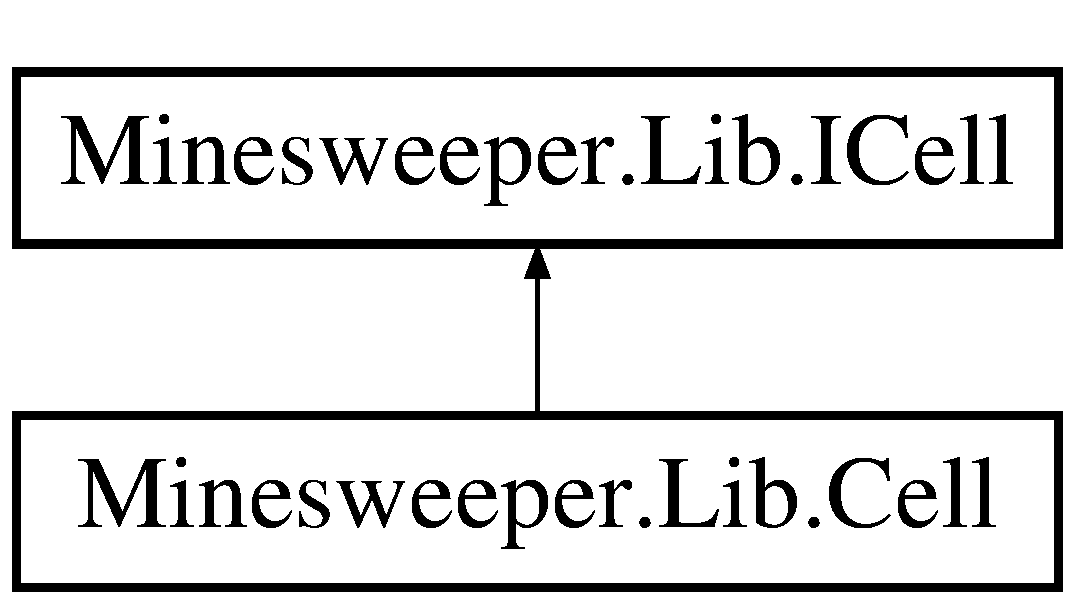
\includegraphics[height=2.000000cm]{class_minesweeper_1_1_lib_1_1_cell}
\end{center}
\end{figure}
\subsection*{Public Member Functions}
\begin{DoxyCompactItemize}
\item 
\hyperlink{class_minesweeper_1_1_lib_1_1_cell_a2dd45aa4466e64696feb140d13cf0899}{Cell} ()
\begin{DoxyCompactList}\small\item\em Initializes a new instance of the \hyperlink{class_minesweeper_1_1_lib_1_1_cell}{Cell} class. \end{DoxyCompactList}\item 
void \hyperlink{class_minesweeper_1_1_lib_1_1_cell_a5fa36c247bd91a482ac46ebf7d2f38b8}{Open\+Cell} ()
\begin{DoxyCompactList}\small\item\em Marks the current cell as opened and removes flags. \end{DoxyCompactList}\item 
void \hyperlink{class_minesweeper_1_1_lib_1_1_cell_a0f959eea2ba69dfa8fcb0ee72e8b33ca}{Toggle\+Flag} ()
\begin{DoxyCompactList}\small\item\em Changes the state of the flag. \end{DoxyCompactList}\item 
void \hyperlink{class_minesweeper_1_1_lib_1_1_cell_a64366640c2cb5425cc73817827d291c4}{Add\+Mine} ()
\begin{DoxyCompactList}\small\item\em Marks the current cell as mined. \end{DoxyCompactList}\item 
void \hyperlink{class_minesweeper_1_1_lib_1_1_cell_ad69f61697ceb611c855f3c4e48f60eb4}{Disarm} ()
\begin{DoxyCompactList}\small\item\em Removes the mine from the current cell. \end{DoxyCompactList}\end{DoxyCompactItemize}
\subsection*{Properties}
\begin{DoxyCompactItemize}
\item 
bool \hyperlink{class_minesweeper_1_1_lib_1_1_cell_a78511856244d5f3ed2c876b94d55fcd3}{Is\+Opened}\hspace{0.3cm}{\ttfamily  \mbox{[}get, set\mbox{]}}
\begin{DoxyCompactList}\small\item\em Gets a value indicating whether the current cell is opened. \end{DoxyCompactList}\item 
bool \hyperlink{class_minesweeper_1_1_lib_1_1_cell_ad0b6f5feaeb0f065246e450f853ada61}{Is\+Flagged}\hspace{0.3cm}{\ttfamily  \mbox{[}get, set\mbox{]}}
\begin{DoxyCompactList}\small\item\em Gets a value indicating whether the current cell is flagged. \end{DoxyCompactList}\item 
bool \hyperlink{class_minesweeper_1_1_lib_1_1_cell_a900f81faa7bcc6021be178401b57763c}{Is\+Mined}\hspace{0.3cm}{\ttfamily  \mbox{[}get, set\mbox{]}}
\begin{DoxyCompactList}\small\item\em Gets a value indicating whether the current cell is mined. \end{DoxyCompactList}\end{DoxyCompactItemize}


\subsection{Detailed Description}
\hyperlink{class_minesweeper_1_1_lib_1_1_cell}{Cell} class which represents the minefield's single cell states. 



\subsection{Constructor \& Destructor Documentation}
\hypertarget{class_minesweeper_1_1_lib_1_1_cell_a2dd45aa4466e64696feb140d13cf0899}{\index{Minesweeper\+::\+Lib\+::\+Cell@{Minesweeper\+::\+Lib\+::\+Cell}!Cell@{Cell}}
\index{Cell@{Cell}!Minesweeper\+::\+Lib\+::\+Cell@{Minesweeper\+::\+Lib\+::\+Cell}}
\subsubsection[{Cell}]{\setlength{\rightskip}{0pt plus 5cm}Minesweeper.\+Lib.\+Cell.\+Cell (
\begin{DoxyParamCaption}
{}
\end{DoxyParamCaption}
)}}\label{class_minesweeper_1_1_lib_1_1_cell_a2dd45aa4466e64696feb140d13cf0899}


Initializes a new instance of the \hyperlink{class_minesweeper_1_1_lib_1_1_cell}{Cell} class. 



\subsection{Member Function Documentation}
\hypertarget{class_minesweeper_1_1_lib_1_1_cell_a64366640c2cb5425cc73817827d291c4}{\index{Minesweeper\+::\+Lib\+::\+Cell@{Minesweeper\+::\+Lib\+::\+Cell}!Add\+Mine@{Add\+Mine}}
\index{Add\+Mine@{Add\+Mine}!Minesweeper\+::\+Lib\+::\+Cell@{Minesweeper\+::\+Lib\+::\+Cell}}
\subsubsection[{Add\+Mine}]{\setlength{\rightskip}{0pt plus 5cm}void Minesweeper.\+Lib.\+Cell.\+Add\+Mine (
\begin{DoxyParamCaption}
{}
\end{DoxyParamCaption}
)}}\label{class_minesweeper_1_1_lib_1_1_cell_a64366640c2cb5425cc73817827d291c4}


Marks the current cell as mined. 



Implements \hyperlink{interface_minesweeper_1_1_lib_1_1_i_cell_a0befb554376beed982e468052e7c0ed6}{Minesweeper.\+Lib.\+I\+Cell}.

\hypertarget{class_minesweeper_1_1_lib_1_1_cell_ad69f61697ceb611c855f3c4e48f60eb4}{\index{Minesweeper\+::\+Lib\+::\+Cell@{Minesweeper\+::\+Lib\+::\+Cell}!Disarm@{Disarm}}
\index{Disarm@{Disarm}!Minesweeper\+::\+Lib\+::\+Cell@{Minesweeper\+::\+Lib\+::\+Cell}}
\subsubsection[{Disarm}]{\setlength{\rightskip}{0pt plus 5cm}void Minesweeper.\+Lib.\+Cell.\+Disarm (
\begin{DoxyParamCaption}
{}
\end{DoxyParamCaption}
)}}\label{class_minesweeper_1_1_lib_1_1_cell_ad69f61697ceb611c855f3c4e48f60eb4}


Removes the mine from the current cell. 



Implements \hyperlink{interface_minesweeper_1_1_lib_1_1_i_cell_a12556fc759e102491c7ce2c432bd0dec}{Minesweeper.\+Lib.\+I\+Cell}.

\hypertarget{class_minesweeper_1_1_lib_1_1_cell_a5fa36c247bd91a482ac46ebf7d2f38b8}{\index{Minesweeper\+::\+Lib\+::\+Cell@{Minesweeper\+::\+Lib\+::\+Cell}!Open\+Cell@{Open\+Cell}}
\index{Open\+Cell@{Open\+Cell}!Minesweeper\+::\+Lib\+::\+Cell@{Minesweeper\+::\+Lib\+::\+Cell}}
\subsubsection[{Open\+Cell}]{\setlength{\rightskip}{0pt plus 5cm}void Minesweeper.\+Lib.\+Cell.\+Open\+Cell (
\begin{DoxyParamCaption}
{}
\end{DoxyParamCaption}
)}}\label{class_minesweeper_1_1_lib_1_1_cell_a5fa36c247bd91a482ac46ebf7d2f38b8}


Marks the current cell as opened and removes flags. 



Implements \hyperlink{interface_minesweeper_1_1_lib_1_1_i_cell_aa7b5d6db30495f23c0aa595e95aa16ae}{Minesweeper.\+Lib.\+I\+Cell}.

\hypertarget{class_minesweeper_1_1_lib_1_1_cell_a0f959eea2ba69dfa8fcb0ee72e8b33ca}{\index{Minesweeper\+::\+Lib\+::\+Cell@{Minesweeper\+::\+Lib\+::\+Cell}!Toggle\+Flag@{Toggle\+Flag}}
\index{Toggle\+Flag@{Toggle\+Flag}!Minesweeper\+::\+Lib\+::\+Cell@{Minesweeper\+::\+Lib\+::\+Cell}}
\subsubsection[{Toggle\+Flag}]{\setlength{\rightskip}{0pt plus 5cm}void Minesweeper.\+Lib.\+Cell.\+Toggle\+Flag (
\begin{DoxyParamCaption}
{}
\end{DoxyParamCaption}
)}}\label{class_minesweeper_1_1_lib_1_1_cell_a0f959eea2ba69dfa8fcb0ee72e8b33ca}


Changes the state of the flag. 



Implements \hyperlink{interface_minesweeper_1_1_lib_1_1_i_cell_acb11d64a47cb3176d2fe42a093958e49}{Minesweeper.\+Lib.\+I\+Cell}.



\subsection{Property Documentation}
\hypertarget{class_minesweeper_1_1_lib_1_1_cell_ad0b6f5feaeb0f065246e450f853ada61}{\index{Minesweeper\+::\+Lib\+::\+Cell@{Minesweeper\+::\+Lib\+::\+Cell}!Is\+Flagged@{Is\+Flagged}}
\index{Is\+Flagged@{Is\+Flagged}!Minesweeper\+::\+Lib\+::\+Cell@{Minesweeper\+::\+Lib\+::\+Cell}}
\subsubsection[{Is\+Flagged}]{\setlength{\rightskip}{0pt plus 5cm}bool Minesweeper.\+Lib.\+Cell.\+Is\+Flagged\hspace{0.3cm}{\ttfamily [get]}, {\ttfamily [set]}}}\label{class_minesweeper_1_1_lib_1_1_cell_ad0b6f5feaeb0f065246e450f853ada61}


Gets a value indicating whether the current cell is flagged. 

True if the current cell is flagged.\hypertarget{class_minesweeper_1_1_lib_1_1_cell_a900f81faa7bcc6021be178401b57763c}{\index{Minesweeper\+::\+Lib\+::\+Cell@{Minesweeper\+::\+Lib\+::\+Cell}!Is\+Mined@{Is\+Mined}}
\index{Is\+Mined@{Is\+Mined}!Minesweeper\+::\+Lib\+::\+Cell@{Minesweeper\+::\+Lib\+::\+Cell}}
\subsubsection[{Is\+Mined}]{\setlength{\rightskip}{0pt plus 5cm}bool Minesweeper.\+Lib.\+Cell.\+Is\+Mined\hspace{0.3cm}{\ttfamily [get]}, {\ttfamily [set]}}}\label{class_minesweeper_1_1_lib_1_1_cell_a900f81faa7bcc6021be178401b57763c}


Gets a value indicating whether the current cell is mined. 

True if the current cell has a mine.\hypertarget{class_minesweeper_1_1_lib_1_1_cell_a78511856244d5f3ed2c876b94d55fcd3}{\index{Minesweeper\+::\+Lib\+::\+Cell@{Minesweeper\+::\+Lib\+::\+Cell}!Is\+Opened@{Is\+Opened}}
\index{Is\+Opened@{Is\+Opened}!Minesweeper\+::\+Lib\+::\+Cell@{Minesweeper\+::\+Lib\+::\+Cell}}
\subsubsection[{Is\+Opened}]{\setlength{\rightskip}{0pt plus 5cm}bool Minesweeper.\+Lib.\+Cell.\+Is\+Opened\hspace{0.3cm}{\ttfamily [get]}, {\ttfamily [set]}}}\label{class_minesweeper_1_1_lib_1_1_cell_a78511856244d5f3ed2c876b94d55fcd3}


Gets a value indicating whether the current cell is opened. 

True if the current cell is opened.

The documentation for this class was generated from the following file\+:\begin{DoxyCompactItemize}
\item 
Minesweeper/\+Minesweeper/\+Minesweeper.\+Lib/Cell.\+cs\end{DoxyCompactItemize}

\hypertarget{struct_minesweeper_1_1_lib_1_1_cell_pos}{\section{Minesweeper.\+Lib.\+Cell\+Pos Struct Reference}
\label{struct_minesweeper_1_1_lib_1_1_cell_pos}\index{Minesweeper.\+Lib.\+Cell\+Pos@{Minesweeper.\+Lib.\+Cell\+Pos}}
}


Holds position by row and column.  


Inheritance diagram for Minesweeper.\+Lib.\+Cell\+Pos\+:\begin{figure}[H]
\begin{center}
\leavevmode
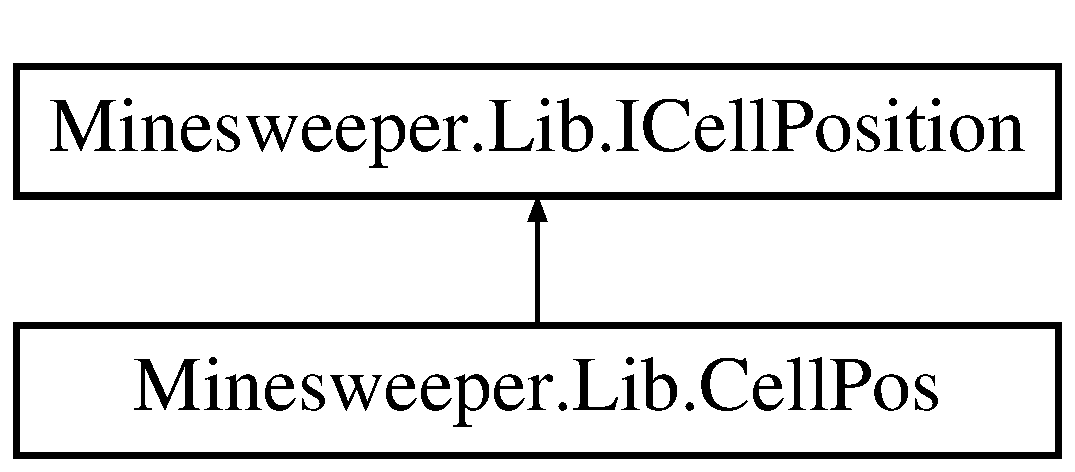
\includegraphics[height=2.000000cm]{struct_minesweeper_1_1_lib_1_1_cell_pos}
\end{center}
\end{figure}
\subsection*{Public Member Functions}
\begin{DoxyCompactItemize}
\item 
\hyperlink{struct_minesweeper_1_1_lib_1_1_cell_pos_afffd1dfab4648433c05d333afdbb563d}{Cell\+Pos} (int initial\+Row, int initial\+Col)
\begin{DoxyCompactList}\small\item\em Initializes a new instance of the \hyperlink{struct_minesweeper_1_1_lib_1_1_cell_pos}{Cell\+Pos} struct. \end{DoxyCompactList}\end{DoxyCompactItemize}
\subsection*{Static Public Attributes}
\begin{DoxyCompactItemize}
\item 
static readonly \hyperlink{struct_minesweeper_1_1_lib_1_1_cell_pos}{Cell\+Pos} \hyperlink{struct_minesweeper_1_1_lib_1_1_cell_pos_a27ef54d6b0afaaf63158d5b270be1afc}{Empty} = new \hyperlink{struct_minesweeper_1_1_lib_1_1_cell_pos}{Cell\+Pos}(0, 0)
\begin{DoxyCompactList}\small\item\em Represents a cell that has Row and Col values set to zero. \end{DoxyCompactList}\end{DoxyCompactItemize}
\subsection*{Properties}
\begin{DoxyCompactItemize}
\item 
int \hyperlink{struct_minesweeper_1_1_lib_1_1_cell_pos_adb4d01bbbda584e580a188aa48173834}{Row}\hspace{0.3cm}{\ttfamily  \mbox{[}get, set\mbox{]}}
\begin{DoxyCompactList}\small\item\em Gets or sets value for position by row. \end{DoxyCompactList}\item 
int \hyperlink{struct_minesweeper_1_1_lib_1_1_cell_pos_a0188f8cda7f5c928a7c0e3f252878da2}{Col}\hspace{0.3cm}{\ttfamily  \mbox{[}get, set\mbox{]}}
\begin{DoxyCompactList}\small\item\em Gets or sets value for position by column. \end{DoxyCompactList}\end{DoxyCompactItemize}


\subsection{Detailed Description}
Holds position by row and column. 



\subsection{Constructor \& Destructor Documentation}
\hypertarget{struct_minesweeper_1_1_lib_1_1_cell_pos_afffd1dfab4648433c05d333afdbb563d}{\index{Minesweeper\+::\+Lib\+::\+Cell\+Pos@{Minesweeper\+::\+Lib\+::\+Cell\+Pos}!Cell\+Pos@{Cell\+Pos}}
\index{Cell\+Pos@{Cell\+Pos}!Minesweeper\+::\+Lib\+::\+Cell\+Pos@{Minesweeper\+::\+Lib\+::\+Cell\+Pos}}
\subsubsection[{Cell\+Pos}]{\setlength{\rightskip}{0pt plus 5cm}Minesweeper.\+Lib.\+Cell\+Pos.\+Cell\+Pos (
\begin{DoxyParamCaption}
\item[{int}]{initial\+Row, }
\item[{int}]{initial\+Col}
\end{DoxyParamCaption}
)}}\label{struct_minesweeper_1_1_lib_1_1_cell_pos_afffd1dfab4648433c05d333afdbb563d}


Initializes a new instance of the \hyperlink{struct_minesweeper_1_1_lib_1_1_cell_pos}{Cell\+Pos} struct. 


\begin{DoxyParams}{Parameters}
{\em initial\+Row} & Position by row.\\
\hline
{\em initial\+Col} & Position by column.\\
\hline
\end{DoxyParams}


\subsection{Member Data Documentation}
\hypertarget{struct_minesweeper_1_1_lib_1_1_cell_pos_a27ef54d6b0afaaf63158d5b270be1afc}{\index{Minesweeper\+::\+Lib\+::\+Cell\+Pos@{Minesweeper\+::\+Lib\+::\+Cell\+Pos}!Empty@{Empty}}
\index{Empty@{Empty}!Minesweeper\+::\+Lib\+::\+Cell\+Pos@{Minesweeper\+::\+Lib\+::\+Cell\+Pos}}
\subsubsection[{Empty}]{\setlength{\rightskip}{0pt plus 5cm}readonly {\bf Cell\+Pos} Minesweeper.\+Lib.\+Cell\+Pos.\+Empty = new {\bf Cell\+Pos}(0, 0)\hspace{0.3cm}{\ttfamily [static]}}}\label{struct_minesweeper_1_1_lib_1_1_cell_pos_a27ef54d6b0afaaf63158d5b270be1afc}


Represents a cell that has Row and Col values set to zero. 



\subsection{Property Documentation}
\hypertarget{struct_minesweeper_1_1_lib_1_1_cell_pos_a0188f8cda7f5c928a7c0e3f252878da2}{\index{Minesweeper\+::\+Lib\+::\+Cell\+Pos@{Minesweeper\+::\+Lib\+::\+Cell\+Pos}!Col@{Col}}
\index{Col@{Col}!Minesweeper\+::\+Lib\+::\+Cell\+Pos@{Minesweeper\+::\+Lib\+::\+Cell\+Pos}}
\subsubsection[{Col}]{\setlength{\rightskip}{0pt plus 5cm}int Minesweeper.\+Lib.\+Cell\+Pos.\+Col\hspace{0.3cm}{\ttfamily [get]}, {\ttfamily [set]}}}\label{struct_minesweeper_1_1_lib_1_1_cell_pos_a0188f8cda7f5c928a7c0e3f252878da2}


Gets or sets value for position by column. 

Position by column.\hypertarget{struct_minesweeper_1_1_lib_1_1_cell_pos_adb4d01bbbda584e580a188aa48173834}{\index{Minesweeper\+::\+Lib\+::\+Cell\+Pos@{Minesweeper\+::\+Lib\+::\+Cell\+Pos}!Row@{Row}}
\index{Row@{Row}!Minesweeper\+::\+Lib\+::\+Cell\+Pos@{Minesweeper\+::\+Lib\+::\+Cell\+Pos}}
\subsubsection[{Row}]{\setlength{\rightskip}{0pt plus 5cm}int Minesweeper.\+Lib.\+Cell\+Pos.\+Row\hspace{0.3cm}{\ttfamily [get]}, {\ttfamily [set]}}}\label{struct_minesweeper_1_1_lib_1_1_cell_pos_adb4d01bbbda584e580a188aa48173834}


Gets or sets value for position by row. 

Position by row.

The documentation for this struct was generated from the following file\+:\begin{DoxyCompactItemize}
\item 
Minesweeper/\+Minesweeper/\+Minesweeper.\+Lib/Cell\+Pos.\+cs\end{DoxyCompactItemize}

\hypertarget{class_minesweeper_1_1_unit_tests_1_1_common_1_1_cell_pos_test}{\section{Minesweeper.\+Unit\+Tests.\+Common.\+Cell\+Pos\+Test Class Reference}
\label{class_minesweeper_1_1_unit_tests_1_1_common_1_1_cell_pos_test}\index{Minesweeper.\+Unit\+Tests.\+Common.\+Cell\+Pos\+Test@{Minesweeper.\+Unit\+Tests.\+Common.\+Cell\+Pos\+Test}}
}
\subsection*{Public Member Functions}
\begin{DoxyCompactItemize}
\item 
\hypertarget{class_minesweeper_1_1_unit_tests_1_1_common_1_1_cell_pos_test_a704f4597ba775711ac847859e4e26102}{void {\bfseries Test\+Initialize} ()}\label{class_minesweeper_1_1_unit_tests_1_1_common_1_1_cell_pos_test_a704f4597ba775711ac847859e4e26102}

\item 
\hypertarget{class_minesweeper_1_1_unit_tests_1_1_common_1_1_cell_pos_test_a86b4b409ca594fec6c5db941bf0b1c8d}{void {\bfseries Test\+Field\+Initialization} ()}\label{class_minesweeper_1_1_unit_tests_1_1_common_1_1_cell_pos_test_a86b4b409ca594fec6c5db941bf0b1c8d}

\item 
\hypertarget{class_minesweeper_1_1_unit_tests_1_1_common_1_1_cell_pos_test_add27578158ad507d72a7a0bcffbb4738}{void {\bfseries Test\+Prop\+Row\+Set\+Negative\+Value} ()}\label{class_minesweeper_1_1_unit_tests_1_1_common_1_1_cell_pos_test_add27578158ad507d72a7a0bcffbb4738}

\item 
\hypertarget{class_minesweeper_1_1_unit_tests_1_1_common_1_1_cell_pos_test_aa38b31c679ca3dd76ce6323d8e04c3c5}{void {\bfseries Test\+Prop\+Col\+Set\+Negative\+Value} ()}\label{class_minesweeper_1_1_unit_tests_1_1_common_1_1_cell_pos_test_aa38b31c679ca3dd76ce6323d8e04c3c5}

\end{DoxyCompactItemize}


The documentation for this class was generated from the following file\+:\begin{DoxyCompactItemize}
\item 
Minesweeper/\+Minesweeper/\+Minesweeper.\+Unit\+Tests/\+Common/Cell\+Pos\+Test.\+cs\end{DoxyCompactItemize}

\hypertarget{class_minesweeper_1_1_unit_tests_1_1_common_1_1_cell_unit_test}{\section{Minesweeper.\+Unit\+Tests.\+Common.\+Cell\+Unit\+Test Class Reference}
\label{class_minesweeper_1_1_unit_tests_1_1_common_1_1_cell_unit_test}\index{Minesweeper.\+Unit\+Tests.\+Common.\+Cell\+Unit\+Test@{Minesweeper.\+Unit\+Tests.\+Common.\+Cell\+Unit\+Test}}
}
\subsection*{Public Member Functions}
\begin{DoxyCompactItemize}
\item 
\hypertarget{class_minesweeper_1_1_unit_tests_1_1_common_1_1_cell_unit_test_a588282b37cb05f2f5c6e61796a600a02}{void {\bfseries Test\+Constructor\+Cell} ()}\label{class_minesweeper_1_1_unit_tests_1_1_common_1_1_cell_unit_test_a588282b37cb05f2f5c6e61796a600a02}

\item 
\hypertarget{class_minesweeper_1_1_unit_tests_1_1_common_1_1_cell_unit_test_ac1ee945d62b5da9e0cc1c8b032561498}{void {\bfseries Test\+Is\+Open\+Property\+Initialization} ()}\label{class_minesweeper_1_1_unit_tests_1_1_common_1_1_cell_unit_test_ac1ee945d62b5da9e0cc1c8b032561498}

\item 
\hypertarget{class_minesweeper_1_1_unit_tests_1_1_common_1_1_cell_unit_test_a41fdb4086cc1af8ba993555a5a461274}{void {\bfseries Test\+Is\+Mined\+Property\+Initialization} ()}\label{class_minesweeper_1_1_unit_tests_1_1_common_1_1_cell_unit_test_a41fdb4086cc1af8ba993555a5a461274}

\item 
\hypertarget{class_minesweeper_1_1_unit_tests_1_1_common_1_1_cell_unit_test_a34004aa69d89969444a6b708fcfeeb1b}{void {\bfseries Test\+Is\+Falgged\+Property\+Initialization} ()}\label{class_minesweeper_1_1_unit_tests_1_1_common_1_1_cell_unit_test_a34004aa69d89969444a6b708fcfeeb1b}

\item 
\hypertarget{class_minesweeper_1_1_unit_tests_1_1_common_1_1_cell_unit_test_af731c81ffc0f3c9069926bbe3a854fc4}{void {\bfseries Test\+Open\+Cell\+Method} ()}\label{class_minesweeper_1_1_unit_tests_1_1_common_1_1_cell_unit_test_af731c81ffc0f3c9069926bbe3a854fc4}

\item 
\hypertarget{class_minesweeper_1_1_unit_tests_1_1_common_1_1_cell_unit_test_a0ae28825bc4e0381a0550a600daca2ec}{void {\bfseries Test\+Toggle\+Flag\+Method} ()}\label{class_minesweeper_1_1_unit_tests_1_1_common_1_1_cell_unit_test_a0ae28825bc4e0381a0550a600daca2ec}

\item 
\hypertarget{class_minesweeper_1_1_unit_tests_1_1_common_1_1_cell_unit_test_a53068361b880d245a7529b3c799dd58d}{void {\bfseries Test\+Add\+Mine\+Method} ()}\label{class_minesweeper_1_1_unit_tests_1_1_common_1_1_cell_unit_test_a53068361b880d245a7529b3c799dd58d}

\end{DoxyCompactItemize}


The documentation for this class was generated from the following file\+:\begin{DoxyCompactItemize}
\item 
Minesweeper/\+Minesweeper/\+Minesweeper.\+Unit\+Tests/\+Common/Cell\+Unit\+Test.\+cs\end{DoxyCompactItemize}

\hypertarget{class_minesweeper_1_1_cmd_boom}{\section{Minesweeper.\+Cmd\+Boom Class Reference}
\label{class_minesweeper_1_1_cmd_boom}\index{Minesweeper.\+Cmd\+Boom@{Minesweeper.\+Cmd\+Boom}}
}


Implements the Execute method by invoking an action on Minesweeper\+Game.  


Inheritance diagram for Minesweeper.\+Cmd\+Boom\+:\begin{figure}[H]
\begin{center}
\leavevmode
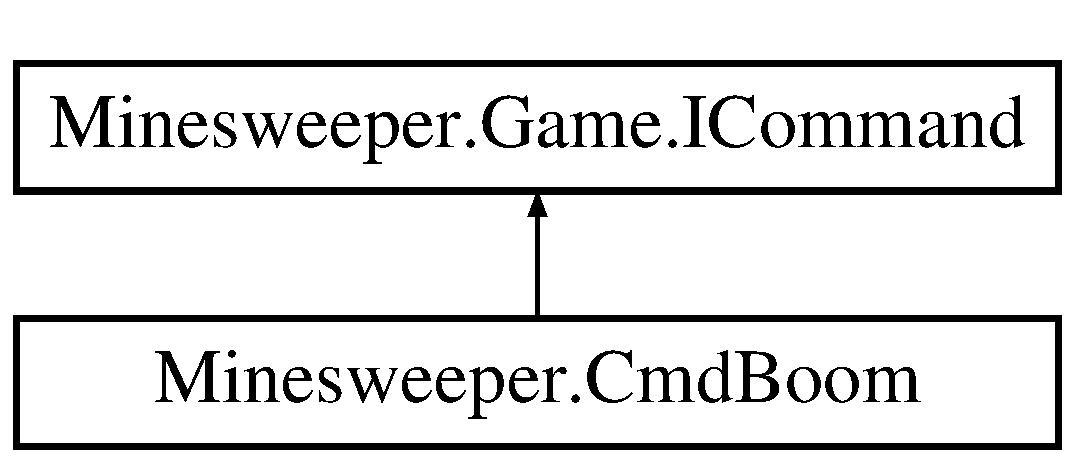
\includegraphics[height=2.000000cm]{class_minesweeper_1_1_cmd_boom}
\end{center}
\end{figure}
\subsection*{Public Member Functions}
\begin{DoxyCompactItemize}
\item 
\hyperlink{class_minesweeper_1_1_cmd_boom_a7d040975d77b1b48c1683b306a70a51e}{Cmd\+Boom} (\hyperlink{class_minesweeper_1_1_game_1_1_minesweeper_game}{Minesweeper\+Game} game)
\begin{DoxyCompactList}\small\item\em Initializes a new instance of the \hyperlink{class_minesweeper_1_1_cmd_boom}{Cmd\+Boom} class. \end{DoxyCompactList}\item 
bool \hyperlink{class_minesweeper_1_1_cmd_boom_ac98aceae68a835b332342321a1a53abe}{Execute} ()
\begin{DoxyCompactList}\small\item\em Invokes the action on the Minesweeper\+Game object. \end{DoxyCompactList}\end{DoxyCompactItemize}


\subsection{Detailed Description}
Implements the Execute method by invoking an action on Minesweeper\+Game. 



\subsection{Constructor \& Destructor Documentation}
\hypertarget{class_minesweeper_1_1_cmd_boom_a7d040975d77b1b48c1683b306a70a51e}{\index{Minesweeper\+::\+Cmd\+Boom@{Minesweeper\+::\+Cmd\+Boom}!Cmd\+Boom@{Cmd\+Boom}}
\index{Cmd\+Boom@{Cmd\+Boom}!Minesweeper\+::\+Cmd\+Boom@{Minesweeper\+::\+Cmd\+Boom}}
\subsubsection[{Cmd\+Boom}]{\setlength{\rightskip}{0pt plus 5cm}Minesweeper.\+Cmd\+Boom.\+Cmd\+Boom (
\begin{DoxyParamCaption}
\item[{{\bf Minesweeper\+Game}}]{game}
\end{DoxyParamCaption}
)}}\label{class_minesweeper_1_1_cmd_boom_a7d040975d77b1b48c1683b306a70a51e}


Initializes a new instance of the \hyperlink{class_minesweeper_1_1_cmd_boom}{Cmd\+Boom} class. 


\begin{DoxyParams}{Parameters}
{\em game} & The Minesweeper\+Game object on which the action will be invoked.\\
\hline
\end{DoxyParams}


\subsection{Member Function Documentation}
\hypertarget{class_minesweeper_1_1_cmd_boom_ac98aceae68a835b332342321a1a53abe}{\index{Minesweeper\+::\+Cmd\+Boom@{Minesweeper\+::\+Cmd\+Boom}!Execute@{Execute}}
\index{Execute@{Execute}!Minesweeper\+::\+Cmd\+Boom@{Minesweeper\+::\+Cmd\+Boom}}
\subsubsection[{Execute}]{\setlength{\rightskip}{0pt plus 5cm}bool Minesweeper.\+Cmd\+Boom.\+Execute (
\begin{DoxyParamCaption}
{}
\end{DoxyParamCaption}
)}}\label{class_minesweeper_1_1_cmd_boom_ac98aceae68a835b332342321a1a53abe}


Invokes the action on the Minesweeper\+Game object. 

\begin{DoxyReturn}{Returns}
Returns true if more commands can be executed.
\end{DoxyReturn}


Implements \hyperlink{interface_minesweeper_1_1_game_1_1_i_command_a03482e68480cad46a8cf419a87440cc9}{Minesweeper.\+Game.\+I\+Command}.



The documentation for this class was generated from the following file\+:\begin{DoxyCompactItemize}
\item 
Minesweeper/\+Minesweeper/\+Minesweeper.\+game/\+Commands/Cmd\+Boom.\+cs\end{DoxyCompactItemize}

\hypertarget{class_minesweeper_1_1_cmd_exit}{\section{Minesweeper.\+Cmd\+Exit Class Reference}
\label{class_minesweeper_1_1_cmd_exit}\index{Minesweeper.\+Cmd\+Exit@{Minesweeper.\+Cmd\+Exit}}
}


Implements the Execute method by invoking an action on Minesweeper\+Game.  


Inheritance diagram for Minesweeper.\+Cmd\+Exit\+:\begin{figure}[H]
\begin{center}
\leavevmode
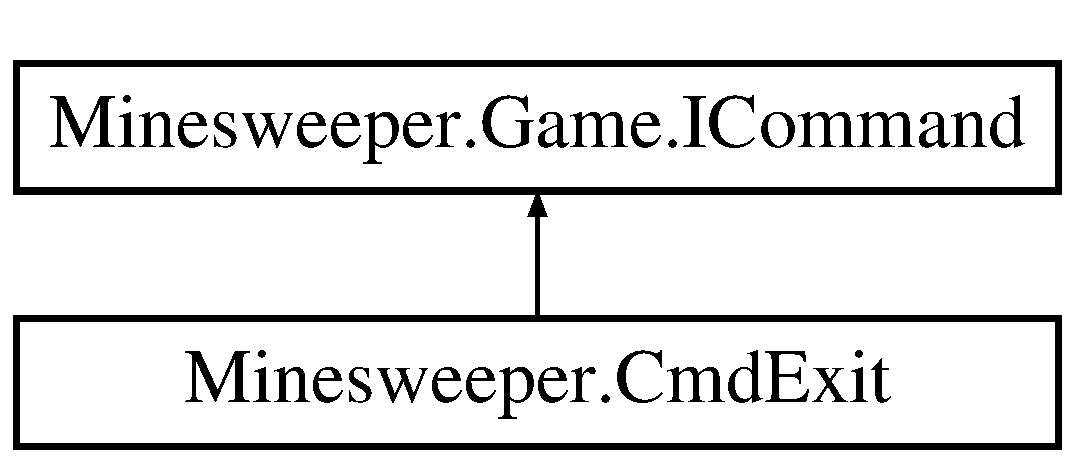
\includegraphics[height=2.000000cm]{class_minesweeper_1_1_cmd_exit}
\end{center}
\end{figure}
\subsection*{Public Member Functions}
\begin{DoxyCompactItemize}
\item 
\hyperlink{class_minesweeper_1_1_cmd_exit_aa7d366e7ba946bbb30a04c374cd8e946}{Cmd\+Exit} (\hyperlink{class_minesweeper_1_1_game_1_1_minesweeper_game}{Minesweeper\+Game} game)
\begin{DoxyCompactList}\small\item\em Initializes a new instance of the \hyperlink{class_minesweeper_1_1_cmd_exit}{Cmd\+Exit} class. \end{DoxyCompactList}\item 
bool \hyperlink{class_minesweeper_1_1_cmd_exit_a218e1498a94ac5b49f0dab48d4f154aa}{Execute} ()
\begin{DoxyCompactList}\small\item\em Invokes the action on the Minesweeper\+Game object. \end{DoxyCompactList}\end{DoxyCompactItemize}


\subsection{Detailed Description}
Implements the Execute method by invoking an action on Minesweeper\+Game. 



\subsection{Constructor \& Destructor Documentation}
\hypertarget{class_minesweeper_1_1_cmd_exit_aa7d366e7ba946bbb30a04c374cd8e946}{\index{Minesweeper\+::\+Cmd\+Exit@{Minesweeper\+::\+Cmd\+Exit}!Cmd\+Exit@{Cmd\+Exit}}
\index{Cmd\+Exit@{Cmd\+Exit}!Minesweeper\+::\+Cmd\+Exit@{Minesweeper\+::\+Cmd\+Exit}}
\subsubsection[{Cmd\+Exit}]{\setlength{\rightskip}{0pt plus 5cm}Minesweeper.\+Cmd\+Exit.\+Cmd\+Exit (
\begin{DoxyParamCaption}
\item[{{\bf Minesweeper\+Game}}]{game}
\end{DoxyParamCaption}
)}}\label{class_minesweeper_1_1_cmd_exit_aa7d366e7ba946bbb30a04c374cd8e946}


Initializes a new instance of the \hyperlink{class_minesweeper_1_1_cmd_exit}{Cmd\+Exit} class. 


\begin{DoxyParams}{Parameters}
{\em game} & The Minesweeper\+Game object on which the action will be invoked.\\
\hline
\end{DoxyParams}


\subsection{Member Function Documentation}
\hypertarget{class_minesweeper_1_1_cmd_exit_a218e1498a94ac5b49f0dab48d4f154aa}{\index{Minesweeper\+::\+Cmd\+Exit@{Minesweeper\+::\+Cmd\+Exit}!Execute@{Execute}}
\index{Execute@{Execute}!Minesweeper\+::\+Cmd\+Exit@{Minesweeper\+::\+Cmd\+Exit}}
\subsubsection[{Execute}]{\setlength{\rightskip}{0pt plus 5cm}bool Minesweeper.\+Cmd\+Exit.\+Execute (
\begin{DoxyParamCaption}
{}
\end{DoxyParamCaption}
)}}\label{class_minesweeper_1_1_cmd_exit_a218e1498a94ac5b49f0dab48d4f154aa}


Invokes the action on the Minesweeper\+Game object. 

\begin{DoxyReturn}{Returns}
Returns true if more commands can be executed.
\end{DoxyReturn}


Implements \hyperlink{interface_minesweeper_1_1_game_1_1_i_command_a03482e68480cad46a8cf419a87440cc9}{Minesweeper.\+Game.\+I\+Command}.



The documentation for this class was generated from the following file\+:\begin{DoxyCompactItemize}
\item 
Minesweeper/\+Minesweeper/\+Minesweeper.\+game/\+Commands/Cmd\+Exit.\+cs\end{DoxyCompactItemize}

\hypertarget{class_minesweeper_1_1_cmd_flag_cell}{\section{Minesweeper.\+Cmd\+Flag\+Cell Class Reference}
\label{class_minesweeper_1_1_cmd_flag_cell}\index{Minesweeper.\+Cmd\+Flag\+Cell@{Minesweeper.\+Cmd\+Flag\+Cell}}
}


Implements the Execute method by invoking an action on Minesweeper\+Game.  


Inheritance diagram for Minesweeper.\+Cmd\+Flag\+Cell\+:\begin{figure}[H]
\begin{center}
\leavevmode
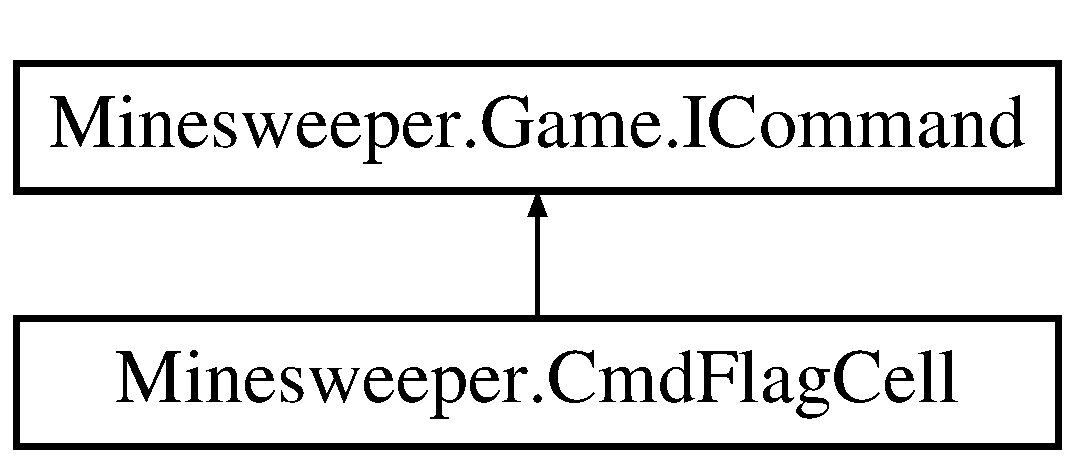
\includegraphics[height=2.000000cm]{class_minesweeper_1_1_cmd_flag_cell}
\end{center}
\end{figure}
\subsection*{Public Member Functions}
\begin{DoxyCompactItemize}
\item 
\hyperlink{class_minesweeper_1_1_cmd_flag_cell_af58abdbee18020bc801f51f5437701e4}{Cmd\+Flag\+Cell} (\hyperlink{class_minesweeper_1_1_game_1_1_minesweeper_game}{Minesweeper\+Game} game, \hyperlink{struct_minesweeper_1_1_lib_1_1_cell_pos}{Cell\+Pos} target\+Cell)
\begin{DoxyCompactList}\small\item\em Initializes a new instance of the \hyperlink{class_minesweeper_1_1_cmd_flag_cell}{Cmd\+Flag\+Cell} class. \end{DoxyCompactList}\item 
bool \hyperlink{class_minesweeper_1_1_cmd_flag_cell_ab8fdee19beed086308829c7d3ae9b7ef}{Execute} ()
\begin{DoxyCompactList}\small\item\em Invokes the action on the Minesweeper\+Game object. \end{DoxyCompactList}\end{DoxyCompactItemize}


\subsection{Detailed Description}
Implements the Execute method by invoking an action on Minesweeper\+Game. 



\subsection{Constructor \& Destructor Documentation}
\hypertarget{class_minesweeper_1_1_cmd_flag_cell_af58abdbee18020bc801f51f5437701e4}{\index{Minesweeper\+::\+Cmd\+Flag\+Cell@{Minesweeper\+::\+Cmd\+Flag\+Cell}!Cmd\+Flag\+Cell@{Cmd\+Flag\+Cell}}
\index{Cmd\+Flag\+Cell@{Cmd\+Flag\+Cell}!Minesweeper\+::\+Cmd\+Flag\+Cell@{Minesweeper\+::\+Cmd\+Flag\+Cell}}
\subsubsection[{Cmd\+Flag\+Cell}]{\setlength{\rightskip}{0pt plus 5cm}Minesweeper.\+Cmd\+Flag\+Cell.\+Cmd\+Flag\+Cell (
\begin{DoxyParamCaption}
\item[{{\bf Minesweeper\+Game}}]{game, }
\item[{{\bf Cell\+Pos}}]{target\+Cell}
\end{DoxyParamCaption}
)}}\label{class_minesweeper_1_1_cmd_flag_cell_af58abdbee18020bc801f51f5437701e4}


Initializes a new instance of the \hyperlink{class_minesweeper_1_1_cmd_flag_cell}{Cmd\+Flag\+Cell} class. 


\begin{DoxyParams}{Parameters}
{\em game} & The Minesweeper\+Game object on which the action will be invoked.\\
\hline
{\em target\+Cell} & The position of the cell on which the action will be invoked.\\
\hline
\end{DoxyParams}


\subsection{Member Function Documentation}
\hypertarget{class_minesweeper_1_1_cmd_flag_cell_ab8fdee19beed086308829c7d3ae9b7ef}{\index{Minesweeper\+::\+Cmd\+Flag\+Cell@{Minesweeper\+::\+Cmd\+Flag\+Cell}!Execute@{Execute}}
\index{Execute@{Execute}!Minesweeper\+::\+Cmd\+Flag\+Cell@{Minesweeper\+::\+Cmd\+Flag\+Cell}}
\subsubsection[{Execute}]{\setlength{\rightskip}{0pt plus 5cm}bool Minesweeper.\+Cmd\+Flag\+Cell.\+Execute (
\begin{DoxyParamCaption}
{}
\end{DoxyParamCaption}
)}}\label{class_minesweeper_1_1_cmd_flag_cell_ab8fdee19beed086308829c7d3ae9b7ef}


Invokes the action on the Minesweeper\+Game object. 

\begin{DoxyReturn}{Returns}
Returns true if more commands can be executed.
\end{DoxyReturn}


Implements \hyperlink{interface_minesweeper_1_1_game_1_1_i_command_a03482e68480cad46a8cf419a87440cc9}{Minesweeper.\+Game.\+I\+Command}.



The documentation for this class was generated from the following file\+:\begin{DoxyCompactItemize}
\item 
Minesweeper/\+Minesweeper/\+Minesweeper.\+game/\+Commands/Cmd\+Flag\+Cell.\+cs\end{DoxyCompactItemize}

\hypertarget{class_minesweeper_1_1_cmd_invalid}{\section{Minesweeper.\+Cmd\+Invalid Class Reference}
\label{class_minesweeper_1_1_cmd_invalid}\index{Minesweeper.\+Cmd\+Invalid@{Minesweeper.\+Cmd\+Invalid}}
}


Implements the Execute method by invoking an action on Minesweeper\+Game.  


Inheritance diagram for Minesweeper.\+Cmd\+Invalid\+:\begin{figure}[H]
\begin{center}
\leavevmode
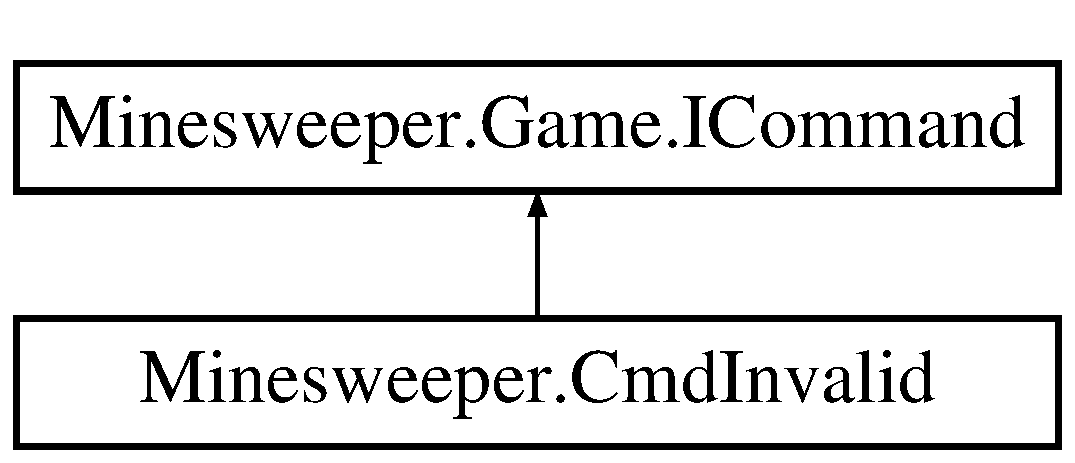
\includegraphics[height=2.000000cm]{class_minesweeper_1_1_cmd_invalid}
\end{center}
\end{figure}
\subsection*{Public Member Functions}
\begin{DoxyCompactItemize}
\item 
\hyperlink{class_minesweeper_1_1_cmd_invalid_a7bfd65d59c12ac6f90b82772e562a288}{Cmd\+Invalid} (\hyperlink{class_minesweeper_1_1_game_1_1_minesweeper_game}{Minesweeper\+Game} game)
\begin{DoxyCompactList}\small\item\em Initializes a new instance of the \hyperlink{class_minesweeper_1_1_cmd_invalid}{Cmd\+Invalid} class. \end{DoxyCompactList}\item 
bool \hyperlink{class_minesweeper_1_1_cmd_invalid_a7d6834d857c3159a20160c2eb94c557e}{Execute} ()
\begin{DoxyCompactList}\small\item\em Invokes the action on the Minesweeper\+Game object. \end{DoxyCompactList}\end{DoxyCompactItemize}


\subsection{Detailed Description}
Implements the Execute method by invoking an action on Minesweeper\+Game. 



\subsection{Constructor \& Destructor Documentation}
\hypertarget{class_minesweeper_1_1_cmd_invalid_a7bfd65d59c12ac6f90b82772e562a288}{\index{Minesweeper\+::\+Cmd\+Invalid@{Minesweeper\+::\+Cmd\+Invalid}!Cmd\+Invalid@{Cmd\+Invalid}}
\index{Cmd\+Invalid@{Cmd\+Invalid}!Minesweeper\+::\+Cmd\+Invalid@{Minesweeper\+::\+Cmd\+Invalid}}
\subsubsection[{Cmd\+Invalid}]{\setlength{\rightskip}{0pt plus 5cm}Minesweeper.\+Cmd\+Invalid.\+Cmd\+Invalid (
\begin{DoxyParamCaption}
\item[{{\bf Minesweeper\+Game}}]{game}
\end{DoxyParamCaption}
)}}\label{class_minesweeper_1_1_cmd_invalid_a7bfd65d59c12ac6f90b82772e562a288}


Initializes a new instance of the \hyperlink{class_minesweeper_1_1_cmd_invalid}{Cmd\+Invalid} class. 


\begin{DoxyParams}{Parameters}
{\em game} & The Minesweeper\+Game object on which the action will be invoked.\\
\hline
\end{DoxyParams}


\subsection{Member Function Documentation}
\hypertarget{class_minesweeper_1_1_cmd_invalid_a7d6834d857c3159a20160c2eb94c557e}{\index{Minesweeper\+::\+Cmd\+Invalid@{Minesweeper\+::\+Cmd\+Invalid}!Execute@{Execute}}
\index{Execute@{Execute}!Minesweeper\+::\+Cmd\+Invalid@{Minesweeper\+::\+Cmd\+Invalid}}
\subsubsection[{Execute}]{\setlength{\rightskip}{0pt plus 5cm}bool Minesweeper.\+Cmd\+Invalid.\+Execute (
\begin{DoxyParamCaption}
{}
\end{DoxyParamCaption}
)}}\label{class_minesweeper_1_1_cmd_invalid_a7d6834d857c3159a20160c2eb94c557e}


Invokes the action on the Minesweeper\+Game object. 

\begin{DoxyReturn}{Returns}
Returns true if more commands can be executed.
\end{DoxyReturn}


Implements \hyperlink{interface_minesweeper_1_1_game_1_1_i_command_a03482e68480cad46a8cf419a87440cc9}{Minesweeper.\+Game.\+I\+Command}.



The documentation for this class was generated from the following file\+:\begin{DoxyCompactItemize}
\item 
Minesweeper/\+Minesweeper/\+Minesweeper.\+game/\+Commands/Cmd\+Invalid.\+cs\end{DoxyCompactItemize}

\hypertarget{class_minesweeper_1_1_cmd_open_cell}{\section{Minesweeper.\+Cmd\+Open\+Cell Class Reference}
\label{class_minesweeper_1_1_cmd_open_cell}\index{Minesweeper.\+Cmd\+Open\+Cell@{Minesweeper.\+Cmd\+Open\+Cell}}
}


Implements the Execute method by invoking an action on Minesweeper\+Game.  


Inheritance diagram for Minesweeper.\+Cmd\+Open\+Cell\+:\begin{figure}[H]
\begin{center}
\leavevmode
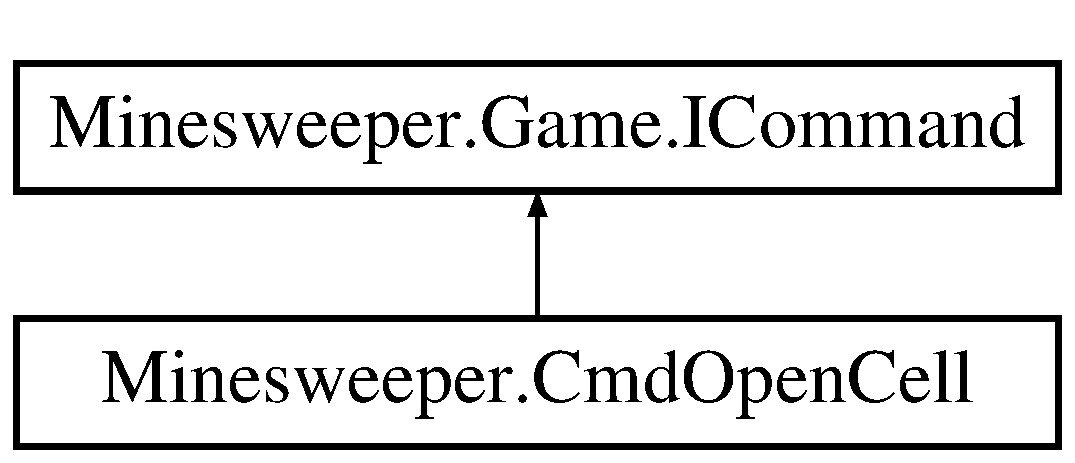
\includegraphics[height=2.000000cm]{class_minesweeper_1_1_cmd_open_cell}
\end{center}
\end{figure}
\subsection*{Public Member Functions}
\begin{DoxyCompactItemize}
\item 
\hyperlink{class_minesweeper_1_1_cmd_open_cell_a36a7f6680ff4e9ef21f09d52f452cdf3}{Cmd\+Open\+Cell} (\hyperlink{class_minesweeper_1_1_game_1_1_minesweeper_game}{Minesweeper\+Game} game, \hyperlink{struct_minesweeper_1_1_lib_1_1_cell_pos}{Cell\+Pos} cell\+To\+Open)
\begin{DoxyCompactList}\small\item\em Initializes a new instance of the \hyperlink{class_minesweeper_1_1_cmd_open_cell}{Cmd\+Open\+Cell} class. \end{DoxyCompactList}\item 
bool \hyperlink{class_minesweeper_1_1_cmd_open_cell_ad8627666ebddf09daf909b3c66173954}{Execute} ()
\begin{DoxyCompactList}\small\item\em Invokes the action on the Minesweeper\+Game object. \end{DoxyCompactList}\end{DoxyCompactItemize}


\subsection{Detailed Description}
Implements the Execute method by invoking an action on Minesweeper\+Game. 



\subsection{Constructor \& Destructor Documentation}
\hypertarget{class_minesweeper_1_1_cmd_open_cell_a36a7f6680ff4e9ef21f09d52f452cdf3}{\index{Minesweeper\+::\+Cmd\+Open\+Cell@{Minesweeper\+::\+Cmd\+Open\+Cell}!Cmd\+Open\+Cell@{Cmd\+Open\+Cell}}
\index{Cmd\+Open\+Cell@{Cmd\+Open\+Cell}!Minesweeper\+::\+Cmd\+Open\+Cell@{Minesweeper\+::\+Cmd\+Open\+Cell}}
\subsubsection[{Cmd\+Open\+Cell}]{\setlength{\rightskip}{0pt plus 5cm}Minesweeper.\+Cmd\+Open\+Cell.\+Cmd\+Open\+Cell (
\begin{DoxyParamCaption}
\item[{{\bf Minesweeper\+Game}}]{game, }
\item[{{\bf Cell\+Pos}}]{cell\+To\+Open}
\end{DoxyParamCaption}
)}}\label{class_minesweeper_1_1_cmd_open_cell_a36a7f6680ff4e9ef21f09d52f452cdf3}


Initializes a new instance of the \hyperlink{class_minesweeper_1_1_cmd_open_cell}{Cmd\+Open\+Cell} class. 


\begin{DoxyParams}{Parameters}
{\em game} & The Minesweeper\+Game object on which the action will be invoked.\\
\hline
{\em cell\+To\+Open} & The position of the cell on which the action will be invoked.\\
\hline
\end{DoxyParams}


\subsection{Member Function Documentation}
\hypertarget{class_minesweeper_1_1_cmd_open_cell_ad8627666ebddf09daf909b3c66173954}{\index{Minesweeper\+::\+Cmd\+Open\+Cell@{Minesweeper\+::\+Cmd\+Open\+Cell}!Execute@{Execute}}
\index{Execute@{Execute}!Minesweeper\+::\+Cmd\+Open\+Cell@{Minesweeper\+::\+Cmd\+Open\+Cell}}
\subsubsection[{Execute}]{\setlength{\rightskip}{0pt plus 5cm}bool Minesweeper.\+Cmd\+Open\+Cell.\+Execute (
\begin{DoxyParamCaption}
{}
\end{DoxyParamCaption}
)}}\label{class_minesweeper_1_1_cmd_open_cell_ad8627666ebddf09daf909b3c66173954}


Invokes the action on the Minesweeper\+Game object. 

\begin{DoxyReturn}{Returns}
Returns true if more commands can be executed.
\end{DoxyReturn}


Implements \hyperlink{interface_minesweeper_1_1_game_1_1_i_command_a03482e68480cad46a8cf419a87440cc9}{Minesweeper.\+Game.\+I\+Command}.



The documentation for this class was generated from the following file\+:\begin{DoxyCompactItemize}
\item 
Minesweeper/\+Minesweeper/\+Minesweeper.\+game/\+Commands/Cmd\+Open\+Cell.\+cs\end{DoxyCompactItemize}

\hypertarget{class_minesweeper_1_1_cmd_restart}{\section{Minesweeper.\+Cmd\+Restart Class Reference}
\label{class_minesweeper_1_1_cmd_restart}\index{Minesweeper.\+Cmd\+Restart@{Minesweeper.\+Cmd\+Restart}}
}


Implements the Execute method by invoking an action on Minesweeper\+Game.  


Inheritance diagram for Minesweeper.\+Cmd\+Restart\+:\begin{figure}[H]
\begin{center}
\leavevmode
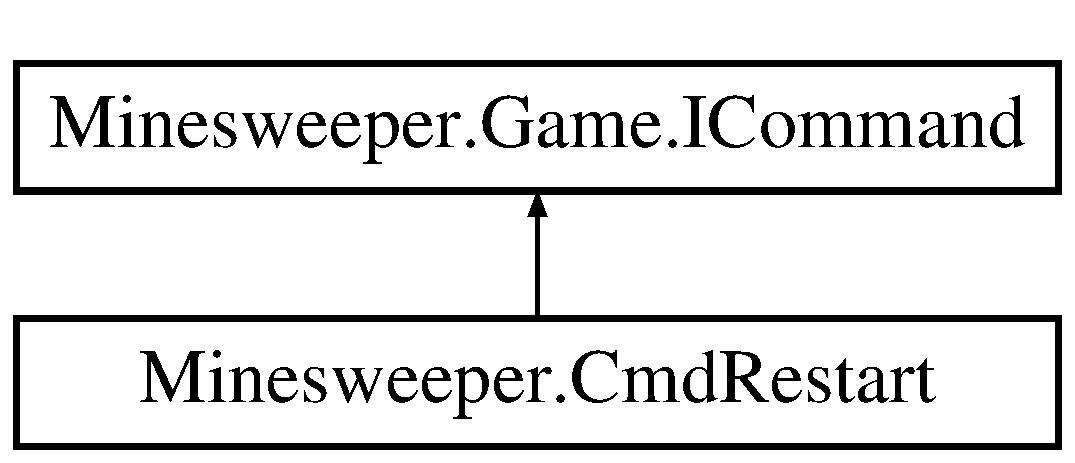
\includegraphics[height=2.000000cm]{class_minesweeper_1_1_cmd_restart}
\end{center}
\end{figure}
\subsection*{Public Member Functions}
\begin{DoxyCompactItemize}
\item 
\hyperlink{class_minesweeper_1_1_cmd_restart_ae20b917dc9b12aafac0e5e5ed5a1a7cc}{Cmd\+Restart} (\hyperlink{class_minesweeper_1_1_game_1_1_minesweeper_game}{Minesweeper\+Game} game)
\begin{DoxyCompactList}\small\item\em Initializes a new instance of the \hyperlink{class_minesweeper_1_1_cmd_restart}{Cmd\+Restart} class. \end{DoxyCompactList}\item 
bool \hyperlink{class_minesweeper_1_1_cmd_restart_a58ff1eea35e4a710c840eedcd421122f}{Execute} ()
\begin{DoxyCompactList}\small\item\em Invokes the action on the Minesweeper\+Game object. \end{DoxyCompactList}\end{DoxyCompactItemize}


\subsection{Detailed Description}
Implements the Execute method by invoking an action on Minesweeper\+Game. 



\subsection{Constructor \& Destructor Documentation}
\hypertarget{class_minesweeper_1_1_cmd_restart_ae20b917dc9b12aafac0e5e5ed5a1a7cc}{\index{Minesweeper\+::\+Cmd\+Restart@{Minesweeper\+::\+Cmd\+Restart}!Cmd\+Restart@{Cmd\+Restart}}
\index{Cmd\+Restart@{Cmd\+Restart}!Minesweeper\+::\+Cmd\+Restart@{Minesweeper\+::\+Cmd\+Restart}}
\subsubsection[{Cmd\+Restart}]{\setlength{\rightskip}{0pt plus 5cm}Minesweeper.\+Cmd\+Restart.\+Cmd\+Restart (
\begin{DoxyParamCaption}
\item[{{\bf Minesweeper\+Game}}]{game}
\end{DoxyParamCaption}
)}}\label{class_minesweeper_1_1_cmd_restart_ae20b917dc9b12aafac0e5e5ed5a1a7cc}


Initializes a new instance of the \hyperlink{class_minesweeper_1_1_cmd_restart}{Cmd\+Restart} class. 


\begin{DoxyParams}{Parameters}
{\em game} & The Minesweeper\+Game object on which the action will be invoked.\\
\hline
\end{DoxyParams}


\subsection{Member Function Documentation}
\hypertarget{class_minesweeper_1_1_cmd_restart_a58ff1eea35e4a710c840eedcd421122f}{\index{Minesweeper\+::\+Cmd\+Restart@{Minesweeper\+::\+Cmd\+Restart}!Execute@{Execute}}
\index{Execute@{Execute}!Minesweeper\+::\+Cmd\+Restart@{Minesweeper\+::\+Cmd\+Restart}}
\subsubsection[{Execute}]{\setlength{\rightskip}{0pt plus 5cm}bool Minesweeper.\+Cmd\+Restart.\+Execute (
\begin{DoxyParamCaption}
{}
\end{DoxyParamCaption}
)}}\label{class_minesweeper_1_1_cmd_restart_a58ff1eea35e4a710c840eedcd421122f}


Invokes the action on the Minesweeper\+Game object. 

\begin{DoxyReturn}{Returns}
Returns true if more commands can be executed.
\end{DoxyReturn}


Implements \hyperlink{interface_minesweeper_1_1_game_1_1_i_command_a03482e68480cad46a8cf419a87440cc9}{Minesweeper.\+Game.\+I\+Command}.



The documentation for this class was generated from the following file\+:\begin{DoxyCompactItemize}
\item 
Minesweeper/\+Minesweeper/\+Minesweeper.\+game/\+Commands/Cmd\+Restart.\+cs\end{DoxyCompactItemize}

\hypertarget{class_minesweeper_1_1_cmd_show_scores}{\section{Minesweeper.\+Cmd\+Show\+Scores Class Reference}
\label{class_minesweeper_1_1_cmd_show_scores}\index{Minesweeper.\+Cmd\+Show\+Scores@{Minesweeper.\+Cmd\+Show\+Scores}}
}


Implements the Execute method by invoking an action on Minesweeper\+Game.  


Inheritance diagram for Minesweeper.\+Cmd\+Show\+Scores\+:\begin{figure}[H]
\begin{center}
\leavevmode
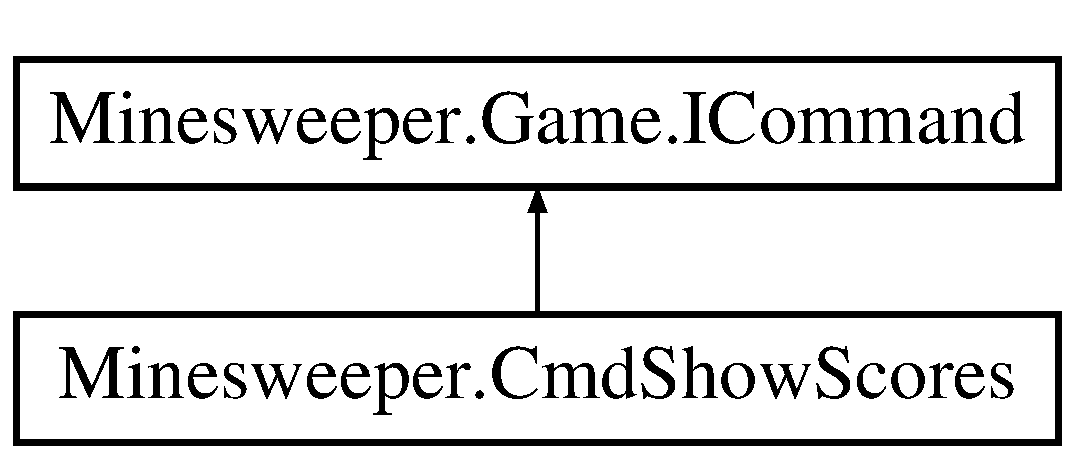
\includegraphics[height=2.000000cm]{class_minesweeper_1_1_cmd_show_scores}
\end{center}
\end{figure}
\subsection*{Public Member Functions}
\begin{DoxyCompactItemize}
\item 
\hyperlink{class_minesweeper_1_1_cmd_show_scores_a00083f6a898ba5324df364c3f38deef4}{Cmd\+Show\+Scores} (\hyperlink{class_minesweeper_1_1_game_1_1_minesweeper_game}{Minesweeper\+Game} game)
\begin{DoxyCompactList}\small\item\em Initializes a new instance of the \hyperlink{class_minesweeper_1_1_cmd_show_scores}{Cmd\+Show\+Scores} class. \end{DoxyCompactList}\item 
bool \hyperlink{class_minesweeper_1_1_cmd_show_scores_ab704f1d09e8802999384c6af9d8d807b}{Execute} ()
\begin{DoxyCompactList}\small\item\em Invokes the action on the Minesweeper\+Game object. \end{DoxyCompactList}\end{DoxyCompactItemize}


\subsection{Detailed Description}
Implements the Execute method by invoking an action on Minesweeper\+Game. 



\subsection{Constructor \& Destructor Documentation}
\hypertarget{class_minesweeper_1_1_cmd_show_scores_a00083f6a898ba5324df364c3f38deef4}{\index{Minesweeper\+::\+Cmd\+Show\+Scores@{Minesweeper\+::\+Cmd\+Show\+Scores}!Cmd\+Show\+Scores@{Cmd\+Show\+Scores}}
\index{Cmd\+Show\+Scores@{Cmd\+Show\+Scores}!Minesweeper\+::\+Cmd\+Show\+Scores@{Minesweeper\+::\+Cmd\+Show\+Scores}}
\subsubsection[{Cmd\+Show\+Scores}]{\setlength{\rightskip}{0pt plus 5cm}Minesweeper.\+Cmd\+Show\+Scores.\+Cmd\+Show\+Scores (
\begin{DoxyParamCaption}
\item[{{\bf Minesweeper\+Game}}]{game}
\end{DoxyParamCaption}
)}}\label{class_minesweeper_1_1_cmd_show_scores_a00083f6a898ba5324df364c3f38deef4}


Initializes a new instance of the \hyperlink{class_minesweeper_1_1_cmd_show_scores}{Cmd\+Show\+Scores} class. 


\begin{DoxyParams}{Parameters}
{\em game} & The Minesweeper\+Game object on which the action will be invoked.\\
\hline
\end{DoxyParams}


\subsection{Member Function Documentation}
\hypertarget{class_minesweeper_1_1_cmd_show_scores_ab704f1d09e8802999384c6af9d8d807b}{\index{Minesweeper\+::\+Cmd\+Show\+Scores@{Minesweeper\+::\+Cmd\+Show\+Scores}!Execute@{Execute}}
\index{Execute@{Execute}!Minesweeper\+::\+Cmd\+Show\+Scores@{Minesweeper\+::\+Cmd\+Show\+Scores}}
\subsubsection[{Execute}]{\setlength{\rightskip}{0pt plus 5cm}bool Minesweeper.\+Cmd\+Show\+Scores.\+Execute (
\begin{DoxyParamCaption}
{}
\end{DoxyParamCaption}
)}}\label{class_minesweeper_1_1_cmd_show_scores_ab704f1d09e8802999384c6af9d8d807b}


Invokes the action on the Minesweeper\+Game object. 

\begin{DoxyReturn}{Returns}
Returns true if more commands can be executed.
\end{DoxyReturn}


Implements \hyperlink{interface_minesweeper_1_1_game_1_1_i_command_a03482e68480cad46a8cf419a87440cc9}{Minesweeper.\+Game.\+I\+Command}.



The documentation for this class was generated from the following file\+:\begin{DoxyCompactItemize}
\item 
Minesweeper/\+Minesweeper/\+Minesweeper.\+game/\+Commands/Cmd\+Show\+Scores.\+cs\end{DoxyCompactItemize}

\hypertarget{class_minesweeper_1_1_game_1_1_command_executor}{\section{Minesweeper.\+Game.\+Command\+Executor Class Reference}
\label{class_minesweeper_1_1_game_1_1_command_executor}\index{Minesweeper.\+Game.\+Command\+Executor@{Minesweeper.\+Game.\+Command\+Executor}}
}


A class which can execute commands of type \hyperlink{interface_minesweeper_1_1_game_1_1_i_command}{Minesweeper.\+Game.\+I\+Command}.  


\subsection*{Public Member Functions}
\begin{DoxyCompactItemize}
\item 
bool \hyperlink{class_minesweeper_1_1_game_1_1_command_executor_a8941c53d834fdcb2e2a6863b1e5f8dcd}{Execute\+Command} (\hyperlink{interface_minesweeper_1_1_game_1_1_i_command}{I\+Command} cmd)
\begin{DoxyCompactList}\small\item\em Executes commands of type \hyperlink{interface_minesweeper_1_1_game_1_1_i_command}{Minesweeper.\+Game.\+I\+Command}. \end{DoxyCompactList}\end{DoxyCompactItemize}


\subsection{Detailed Description}
A class which can execute commands of type \hyperlink{interface_minesweeper_1_1_game_1_1_i_command}{Minesweeper.\+Game.\+I\+Command}. 



\subsection{Member Function Documentation}
\hypertarget{class_minesweeper_1_1_game_1_1_command_executor_a8941c53d834fdcb2e2a6863b1e5f8dcd}{\index{Minesweeper\+::\+Game\+::\+Command\+Executor@{Minesweeper\+::\+Game\+::\+Command\+Executor}!Execute\+Command@{Execute\+Command}}
\index{Execute\+Command@{Execute\+Command}!Minesweeper\+::\+Game\+::\+Command\+Executor@{Minesweeper\+::\+Game\+::\+Command\+Executor}}
\subsubsection[{Execute\+Command}]{\setlength{\rightskip}{0pt plus 5cm}bool Minesweeper.\+Game.\+Command\+Executor.\+Execute\+Command (
\begin{DoxyParamCaption}
\item[{{\bf I\+Command}}]{cmd}
\end{DoxyParamCaption}
)}}\label{class_minesweeper_1_1_game_1_1_command_executor_a8941c53d834fdcb2e2a6863b1e5f8dcd}


Executes commands of type \hyperlink{interface_minesweeper_1_1_game_1_1_i_command}{Minesweeper.\+Game.\+I\+Command}. 


\begin{DoxyParams}{Parameters}
{\em cmd} & The command to execute.\\
\hline
\end{DoxyParams}
\begin{DoxyReturn}{Returns}
Returns true if more commands can be executed.
\end{DoxyReturn}


The documentation for this class was generated from the following file\+:\begin{DoxyCompactItemize}
\item 
Minesweeper/\+Minesweeper/\+Minesweeper.\+game/Command\+Executor.\+cs\end{DoxyCompactItemize}

\hypertarget{class_minesweeper_1_1_unit_tests_1_1_game_1_1_command_executor_test}{\section{Minesweeper.\+Unit\+Tests.\+Game.\+Command\+Executor\+Test Class Reference}
\label{class_minesweeper_1_1_unit_tests_1_1_game_1_1_command_executor_test}\index{Minesweeper.\+Unit\+Tests.\+Game.\+Command\+Executor\+Test@{Minesweeper.\+Unit\+Tests.\+Game.\+Command\+Executor\+Test}}
}
\subsection*{Public Member Functions}
\begin{DoxyCompactItemize}
\item 
\hypertarget{class_minesweeper_1_1_unit_tests_1_1_game_1_1_command_executor_test_aff012c5a3aa7de383757f4acc7bdc25b}{void {\bfseries Test\+\_\+\+Execute\+Command\+With\+Null\+\_\+\+Throws\+Ex} ()}\label{class_minesweeper_1_1_unit_tests_1_1_game_1_1_command_executor_test_aff012c5a3aa7de383757f4acc7bdc25b}

\item 
\hypertarget{class_minesweeper_1_1_unit_tests_1_1_game_1_1_command_executor_test_a49bbecf2083e7cd6a3ee605b87744aab}{void {\bfseries Test\+\_\+\+Execute\+Command\+With\+Valid\+Param} ()}\label{class_minesweeper_1_1_unit_tests_1_1_game_1_1_command_executor_test_a49bbecf2083e7cd6a3ee605b87744aab}

\end{DoxyCompactItemize}


The documentation for this class was generated from the following file\+:\begin{DoxyCompactItemize}
\item 
Minesweeper/\+Minesweeper/\+Minesweeper.\+Unit\+Tests/\+Game/Command\+Executor\+Test.\+cs\end{DoxyCompactItemize}

\hypertarget{class_minesweeper_1_1_game_1_1_command_parser}{\section{Minesweeper.\+Game.\+Command\+Parser Class Reference}
\label{class_minesweeper_1_1_game_1_1_command_parser}\index{Minesweeper.\+Game.\+Command\+Parser@{Minesweeper.\+Game.\+Command\+Parser}}
}


A class that can parse string input and return a command of type \hyperlink{interface_minesweeper_1_1_game_1_1_i_command}{I\+Command}.  


\subsection*{Public Member Functions}
\begin{DoxyCompactItemize}
\item 
\hyperlink{class_minesweeper_1_1_game_1_1_command_parser_a2a6a51a7b7f582d80bc407f04867b9ea}{Command\+Parser} (\hyperlink{class_minesweeper_1_1_game_1_1_minesweeper_game}{Minesweeper\+Game} game)
\begin{DoxyCompactList}\small\item\em Initializes a new instance of the \hyperlink{class_minesweeper_1_1_game_1_1_command_parser}{Command\+Parser} class. \end{DoxyCompactList}\item 
virtual \hyperlink{interface_minesweeper_1_1_game_1_1_i_command}{I\+Command} \hyperlink{class_minesweeper_1_1_game_1_1_command_parser_ab31a5ac6a98e37117d0801cef6c9a188}{Parse\+Command} (string input)
\begin{DoxyCompactList}\small\item\em Parses a string and returns its corresponding \hyperlink{interface_minesweeper_1_1_game_1_1_i_command}{I\+Command}. \end{DoxyCompactList}\end{DoxyCompactItemize}
\subsection*{Properties}
\begin{DoxyCompactItemize}
\item 
\hyperlink{class_minesweeper_1_1_game_1_1_minesweeper_game}{Minesweeper\+Game} \hyperlink{class_minesweeper_1_1_game_1_1_command_parser_ad8ac44210715f94c2d35e94b7ca48a3a}{Game}\hspace{0.3cm}{\ttfamily  \mbox{[}get, set\mbox{]}}
\begin{DoxyCompactList}\small\item\em Gets for the \hyperlink{class_minesweeper_1_1_game_1_1_minesweeper_game}{Minesweeper\+Game} object for which commands will be parsed. \end{DoxyCompactList}\end{DoxyCompactItemize}


\subsection{Detailed Description}
A class that can parse string input and return a command of type \hyperlink{interface_minesweeper_1_1_game_1_1_i_command}{I\+Command}. 



\subsection{Constructor \& Destructor Documentation}
\hypertarget{class_minesweeper_1_1_game_1_1_command_parser_a2a6a51a7b7f582d80bc407f04867b9ea}{\index{Minesweeper\+::\+Game\+::\+Command\+Parser@{Minesweeper\+::\+Game\+::\+Command\+Parser}!Command\+Parser@{Command\+Parser}}
\index{Command\+Parser@{Command\+Parser}!Minesweeper\+::\+Game\+::\+Command\+Parser@{Minesweeper\+::\+Game\+::\+Command\+Parser}}
\subsubsection[{Command\+Parser}]{\setlength{\rightskip}{0pt plus 5cm}Minesweeper.\+Game.\+Command\+Parser.\+Command\+Parser (
\begin{DoxyParamCaption}
\item[{{\bf Minesweeper\+Game}}]{game}
\end{DoxyParamCaption}
)}}\label{class_minesweeper_1_1_game_1_1_command_parser_a2a6a51a7b7f582d80bc407f04867b9ea}


Initializes a new instance of the \hyperlink{class_minesweeper_1_1_game_1_1_command_parser}{Command\+Parser} class. 


\begin{DoxyParams}{Parameters}
{\em game} & The \hyperlink{class_minesweeper_1_1_game_1_1_minesweeper_game}{Minesweeper\+Game} object for which commands will be returned.\\
\hline
\end{DoxyParams}


\subsection{Member Function Documentation}
\hypertarget{class_minesweeper_1_1_game_1_1_command_parser_ab31a5ac6a98e37117d0801cef6c9a188}{\index{Minesweeper\+::\+Game\+::\+Command\+Parser@{Minesweeper\+::\+Game\+::\+Command\+Parser}!Parse\+Command@{Parse\+Command}}
\index{Parse\+Command@{Parse\+Command}!Minesweeper\+::\+Game\+::\+Command\+Parser@{Minesweeper\+::\+Game\+::\+Command\+Parser}}
\subsubsection[{Parse\+Command}]{\setlength{\rightskip}{0pt plus 5cm}virtual {\bf I\+Command} Minesweeper.\+Game.\+Command\+Parser.\+Parse\+Command (
\begin{DoxyParamCaption}
\item[{string}]{input}
\end{DoxyParamCaption}
)\hspace{0.3cm}{\ttfamily [virtual]}}}\label{class_minesweeper_1_1_game_1_1_command_parser_ab31a5ac6a98e37117d0801cef6c9a188}


Parses a string and returns its corresponding \hyperlink{interface_minesweeper_1_1_game_1_1_i_command}{I\+Command}. 


\begin{DoxyParams}{Parameters}
{\em input} & The string to parse.\\
\hline
\end{DoxyParams}
\begin{DoxyReturn}{Returns}
The parsed command.
\end{DoxyReturn}


\subsection{Property Documentation}
\hypertarget{class_minesweeper_1_1_game_1_1_command_parser_ad8ac44210715f94c2d35e94b7ca48a3a}{\index{Minesweeper\+::\+Game\+::\+Command\+Parser@{Minesweeper\+::\+Game\+::\+Command\+Parser}!Game@{Game}}
\index{Game@{Game}!Minesweeper\+::\+Game\+::\+Command\+Parser@{Minesweeper\+::\+Game\+::\+Command\+Parser}}
\subsubsection[{Game}]{\setlength{\rightskip}{0pt plus 5cm}{\bf Minesweeper\+Game} Minesweeper.\+Game.\+Command\+Parser.\+Game\hspace{0.3cm}{\ttfamily [get]}, {\ttfamily [set]}, {\ttfamily [protected]}}}\label{class_minesweeper_1_1_game_1_1_command_parser_ad8ac44210715f94c2d35e94b7ca48a3a}


Gets for the \hyperlink{class_minesweeper_1_1_game_1_1_minesweeper_game}{Minesweeper\+Game} object for which commands will be parsed. 

The \hyperlink{class_minesweeper_1_1_game_1_1_minesweeper_game}{Minesweeper\+Game} property gets the value of the \hyperlink{class_minesweeper_1_1_game_1_1_minesweeper_game}{Minesweeper\+Game} field, game.

The documentation for this class was generated from the following file\+:\begin{DoxyCompactItemize}
\item 
Minesweeper/\+Minesweeper/\+Minesweeper.\+game/Command\+Parser.\+cs\end{DoxyCompactItemize}

\hypertarget{class_minesweeper_1_1_unit_tests_1_1_game_1_1_command_parser_test}{\section{Minesweeper.\+Unit\+Tests.\+Game.\+Command\+Parser\+Test Class Reference}
\label{class_minesweeper_1_1_unit_tests_1_1_game_1_1_command_parser_test}\index{Minesweeper.\+Unit\+Tests.\+Game.\+Command\+Parser\+Test@{Minesweeper.\+Unit\+Tests.\+Game.\+Command\+Parser\+Test}}
}
\subsection*{Public Member Functions}
\begin{DoxyCompactItemize}
\item 
\hypertarget{class_minesweeper_1_1_unit_tests_1_1_game_1_1_command_parser_test_aba7a6ca5a792ec858aceea6c6d4f8e46}{void {\bfseries Test\+Initialize} ()}\label{class_minesweeper_1_1_unit_tests_1_1_game_1_1_command_parser_test_aba7a6ca5a792ec858aceea6c6d4f8e46}

\item 
\hypertarget{class_minesweeper_1_1_unit_tests_1_1_game_1_1_command_parser_test_a11b510a6589053e1de8ae4cfaf1f67e9}{void {\bfseries Test\+\_\+\+Command\+Parser\+\_\+\+Ctor\+With\+Null\+Throws\+Ex} ()}\label{class_minesweeper_1_1_unit_tests_1_1_game_1_1_command_parser_test_a11b510a6589053e1de8ae4cfaf1f67e9}

\item 
\hypertarget{class_minesweeper_1_1_unit_tests_1_1_game_1_1_command_parser_test_a1af3ff2c9e6e18615de38089240ce0b3}{void {\bfseries Test\+\_\+\+Parse\+Command\+\_\+\+Invalid\+Commands} ()}\label{class_minesweeper_1_1_unit_tests_1_1_game_1_1_command_parser_test_a1af3ff2c9e6e18615de38089240ce0b3}

\item 
\hypertarget{class_minesweeper_1_1_unit_tests_1_1_game_1_1_command_parser_test_a79b045882d2d59228762410c34618ff3}{void {\bfseries Test\+\_\+\+Parse\+Command\+\_\+\+Single\+Word\+Commands} ()}\label{class_minesweeper_1_1_unit_tests_1_1_game_1_1_command_parser_test_a79b045882d2d59228762410c34618ff3}

\item 
\hypertarget{class_minesweeper_1_1_unit_tests_1_1_game_1_1_command_parser_test_aadf10189d8655ce986f59259ab919db9}{void {\bfseries Test\+\_\+\+Parse\+Command\+\_\+\+Open\+And\+Flag\+Cell} ()}\label{class_minesweeper_1_1_unit_tests_1_1_game_1_1_command_parser_test_aadf10189d8655ce986f59259ab919db9}

\end{DoxyCompactItemize}


The documentation for this class was generated from the following file\+:\begin{DoxyCompactItemize}
\item 
Minesweeper/\+Minesweeper/\+Minesweeper.\+Unit\+Tests/\+Game/Command\+Parser\+Test.\+cs\end{DoxyCompactItemize}

\hypertarget{class_minesweeper_1_1_unit_tests_1_1_game_1_1_commands_1_1_commands_tests}{\section{Minesweeper.\+Unit\+Tests.\+Game.\+Commands.\+Commands\+Tests Class Reference}
\label{class_minesweeper_1_1_unit_tests_1_1_game_1_1_commands_1_1_commands_tests}\index{Minesweeper.\+Unit\+Tests.\+Game.\+Commands.\+Commands\+Tests@{Minesweeper.\+Unit\+Tests.\+Game.\+Commands.\+Commands\+Tests}}
}
\subsection*{Public Member Functions}
\begin{DoxyCompactItemize}
\item 
\hypertarget{class_minesweeper_1_1_unit_tests_1_1_game_1_1_commands_1_1_commands_tests_a1bd4551d35bee81e4550e1eda22466ec}{void {\bfseries Test\+\_\+\+Cmd\+Boom\+\_\+\+Ctor\+With\+Null\+Throws\+Ex} ()}\label{class_minesweeper_1_1_unit_tests_1_1_game_1_1_commands_1_1_commands_tests_a1bd4551d35bee81e4550e1eda22466ec}

\item 
\hypertarget{class_minesweeper_1_1_unit_tests_1_1_game_1_1_commands_1_1_commands_tests_afcae14159d72a59ca53366145bd32c30}{void {\bfseries Test\+\_\+\+Cmd\+Show\+\_\+\+Ctor\+With\+Null\+Throws\+Ex} ()}\label{class_minesweeper_1_1_unit_tests_1_1_game_1_1_commands_1_1_commands_tests_afcae14159d72a59ca53366145bd32c30}

\item 
\hypertarget{class_minesweeper_1_1_unit_tests_1_1_game_1_1_commands_1_1_commands_tests_a9bcd3fb509b659db7f9c5dc96897e5a9}{void {\bfseries Test\+\_\+\+Cmd\+Restart\+\_\+\+Ctor\+With\+Null\+Throws\+Ex} ()}\label{class_minesweeper_1_1_unit_tests_1_1_game_1_1_commands_1_1_commands_tests_a9bcd3fb509b659db7f9c5dc96897e5a9}

\item 
\hypertarget{class_minesweeper_1_1_unit_tests_1_1_game_1_1_commands_1_1_commands_tests_a870d78a61e7d6cfb10e0ad4ea1d13c03}{void {\bfseries Test\+\_\+\+Cmd\+Invalid\+\_\+\+Ctor\+With\+Null\+Throws\+Ex} ()}\label{class_minesweeper_1_1_unit_tests_1_1_game_1_1_commands_1_1_commands_tests_a870d78a61e7d6cfb10e0ad4ea1d13c03}

\item 
\hypertarget{class_minesweeper_1_1_unit_tests_1_1_game_1_1_commands_1_1_commands_tests_a7e27972f284327380527208834fa903e}{void {\bfseries Test\+\_\+\+Cmd\+Exit\+\_\+\+Ctor\+With\+Null\+Throws\+Ex} ()}\label{class_minesweeper_1_1_unit_tests_1_1_game_1_1_commands_1_1_commands_tests_a7e27972f284327380527208834fa903e}

\item 
\hypertarget{class_minesweeper_1_1_unit_tests_1_1_game_1_1_commands_1_1_commands_tests_aedb9474380b16ce63f0d2986975a0154}{void {\bfseries Test\+\_\+\+Cmd\+Flag\+Cell\+\_\+\+Ctor\+With\+Null\+Throws\+Ex} ()}\label{class_minesweeper_1_1_unit_tests_1_1_game_1_1_commands_1_1_commands_tests_aedb9474380b16ce63f0d2986975a0154}

\item 
\hypertarget{class_minesweeper_1_1_unit_tests_1_1_game_1_1_commands_1_1_commands_tests_aa130704d7271e93eb314ff3d1efe4a0f}{void {\bfseries Test\+\_\+\+Cmd\+Open\+Cell\+\_\+\+Ctor\+With\+Null\+Throws\+Ex} ()}\label{class_minesweeper_1_1_unit_tests_1_1_game_1_1_commands_1_1_commands_tests_aa130704d7271e93eb314ff3d1efe4a0f}

\end{DoxyCompactItemize}


The documentation for this class was generated from the following file\+:\begin{DoxyCompactItemize}
\item 
Minesweeper/\+Minesweeper/\+Minesweeper.\+Unit\+Tests/\+Game/Commands\+Tests.\+cs\end{DoxyCompactItemize}

\hypertarget{class_minesweeper_1_1_lib_1_1_console_reader}{\section{Minesweeper.\+Lib.\+Console\+Reader Class Reference}
\label{class_minesweeper_1_1_lib_1_1_console_reader}\index{Minesweeper.\+Lib.\+Console\+Reader@{Minesweeper.\+Lib.\+Console\+Reader}}
}


Implements the \hyperlink{interface_minesweeper_1_1_lib_1_1_i_user_input_reader}{I\+User\+Input\+Reader} interface with the System.\+Console.  


Inheritance diagram for Minesweeper.\+Lib.\+Console\+Reader\+:\begin{figure}[H]
\begin{center}
\leavevmode
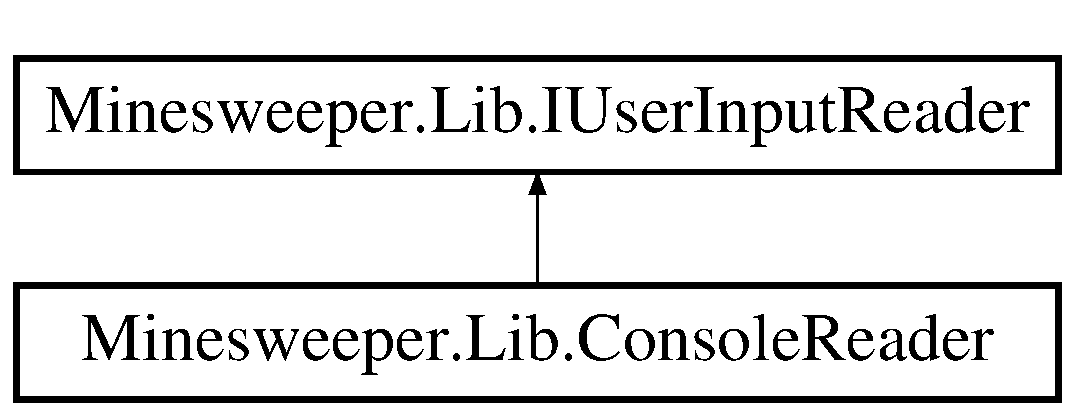
\includegraphics[height=2.000000cm]{class_minesweeper_1_1_lib_1_1_console_reader}
\end{center}
\end{figure}
\subsection*{Public Member Functions}
\begin{DoxyCompactItemize}
\item 
void \hyperlink{class_minesweeper_1_1_lib_1_1_console_reader_a92588508515c5082d628e9f56672e863}{Wait\+For\+Key} ()
\begin{DoxyCompactList}\small\item\em Waits for the user to press a key. \end{DoxyCompactList}\item 
string \hyperlink{class_minesweeper_1_1_lib_1_1_console_reader_ae6bb2ed667d1290078a0f9bb7b53e9a8}{Read\+Line} ()
\begin{DoxyCompactList}\small\item\em Reads the next line of characters from the standard input stream. \end{DoxyCompactList}\end{DoxyCompactItemize}


\subsection{Detailed Description}
Implements the \hyperlink{interface_minesweeper_1_1_lib_1_1_i_user_input_reader}{I\+User\+Input\+Reader} interface with the System.\+Console. 



\subsection{Member Function Documentation}
\hypertarget{class_minesweeper_1_1_lib_1_1_console_reader_ae6bb2ed667d1290078a0f9bb7b53e9a8}{\index{Minesweeper\+::\+Lib\+::\+Console\+Reader@{Minesweeper\+::\+Lib\+::\+Console\+Reader}!Read\+Line@{Read\+Line}}
\index{Read\+Line@{Read\+Line}!Minesweeper\+::\+Lib\+::\+Console\+Reader@{Minesweeper\+::\+Lib\+::\+Console\+Reader}}
\subsubsection[{Read\+Line}]{\setlength{\rightskip}{0pt plus 5cm}string Minesweeper.\+Lib.\+Console\+Reader.\+Read\+Line (
\begin{DoxyParamCaption}
{}
\end{DoxyParamCaption}
)}}\label{class_minesweeper_1_1_lib_1_1_console_reader_ae6bb2ed667d1290078a0f9bb7b53e9a8}


Reads the next line of characters from the standard input stream. 

\begin{DoxyReturn}{Returns}
The next line of characters from the input stream, or null if no more lines are available.
\end{DoxyReturn}


Implements \hyperlink{interface_minesweeper_1_1_lib_1_1_i_user_input_reader_a58da9817d2e63a510cf833ce7d65f008}{Minesweeper.\+Lib.\+I\+User\+Input\+Reader}.

\hypertarget{class_minesweeper_1_1_lib_1_1_console_reader_a92588508515c5082d628e9f56672e863}{\index{Minesweeper\+::\+Lib\+::\+Console\+Reader@{Minesweeper\+::\+Lib\+::\+Console\+Reader}!Wait\+For\+Key@{Wait\+For\+Key}}
\index{Wait\+For\+Key@{Wait\+For\+Key}!Minesweeper\+::\+Lib\+::\+Console\+Reader@{Minesweeper\+::\+Lib\+::\+Console\+Reader}}
\subsubsection[{Wait\+For\+Key}]{\setlength{\rightskip}{0pt plus 5cm}void Minesweeper.\+Lib.\+Console\+Reader.\+Wait\+For\+Key (
\begin{DoxyParamCaption}
{}
\end{DoxyParamCaption}
)}}\label{class_minesweeper_1_1_lib_1_1_console_reader_a92588508515c5082d628e9f56672e863}


Waits for the user to press a key. 



Implements \hyperlink{interface_minesweeper_1_1_lib_1_1_i_user_input_reader_a54b4a65a7cea8be31dc99a6330be6f51}{Minesweeper.\+Lib.\+I\+User\+Input\+Reader}.



The documentation for this class was generated from the following file\+:\begin{DoxyCompactItemize}
\item 
Minesweeper/\+Minesweeper/\+Minesweeper.\+Lib/Console\+Reader.\+cs\end{DoxyCompactItemize}

\hypertarget{class_minesweeper_1_1_lib_1_1_console_renderer}{\section{Minesweeper.\+Lib.\+Console\+Renderer Class Reference}
\label{class_minesweeper_1_1_lib_1_1_console_renderer}\index{Minesweeper.\+Lib.\+Console\+Renderer@{Minesweeper.\+Lib.\+Console\+Renderer}}
}


Writes text messages to the standard output stream.  


Inheritance diagram for Minesweeper.\+Lib.\+Console\+Renderer\+:\begin{figure}[H]
\begin{center}
\leavevmode
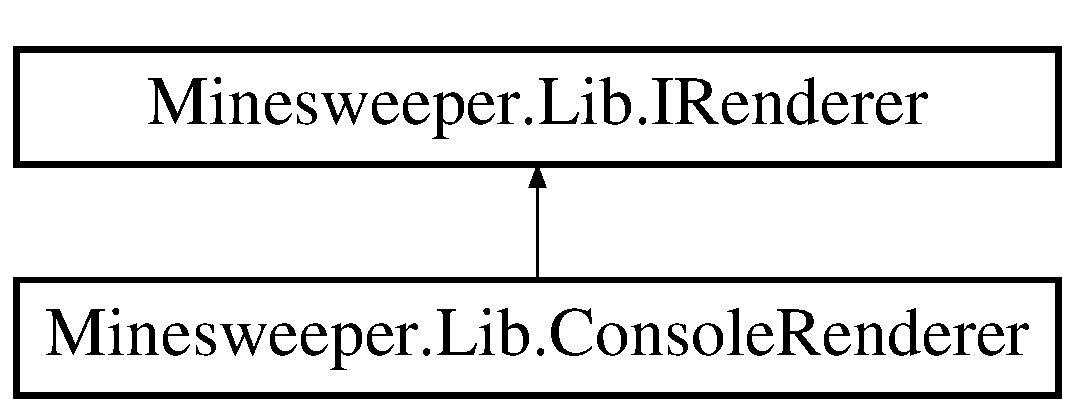
\includegraphics[height=2.000000cm]{class_minesweeper_1_1_lib_1_1_console_renderer}
\end{center}
\end{figure}
\subsection*{Public Member Functions}
\begin{DoxyCompactItemize}
\item 
void \hyperlink{class_minesweeper_1_1_lib_1_1_console_renderer_a0a9b86365042b44de6c5b9da7b40dafe}{Write\+Line} ()
\begin{DoxyCompactList}\small\item\em Writes the current line terminator to the standard output stream. \end{DoxyCompactList}\item 
void \hyperlink{class_minesweeper_1_1_lib_1_1_console_renderer_afe92f94092a0a7876ec1c845ee7d78cf}{Write\+Line} (string format, params object\mbox{[}$\,$\mbox{]} args)
\begin{DoxyCompactList}\small\item\em Writes the text representation of the specified array of objects to the standard output stream using the specified format information, followed by the current line terminator. \end{DoxyCompactList}\item 
void \hyperlink{class_minesweeper_1_1_lib_1_1_console_renderer_a14f9db3445bb4f3921eada8463617e35}{Write} (string format, params object\mbox{[}$\,$\mbox{]} args)
\begin{DoxyCompactList}\small\item\em Writes the text representation of the specified array of objects to the standard output stream using the specified format information. \end{DoxyCompactList}\item 
void \hyperlink{class_minesweeper_1_1_lib_1_1_console_renderer_aa8ccd90c8c5a4e6bb02da7b546ef9c26}{Write\+At} (int left, int top, string format, params object\mbox{[}$\,$\mbox{]} args)
\begin{DoxyCompactList}\small\item\em Writes the text representation of the specified array of objects to the standard output stream using the specified format information at a specific position. \end{DoxyCompactList}\item 
void \hyperlink{class_minesweeper_1_1_lib_1_1_console_renderer_a4968ccf049f1704753728368a2519fe2}{Clear\+Lines} (int left, int top, int num\+Lines)
\begin{DoxyCompactList}\small\item\em Clear specific number of lines. \end{DoxyCompactList}\end{DoxyCompactItemize}


\subsection{Detailed Description}
Writes text messages to the standard output stream. 



\subsection{Member Function Documentation}
\hypertarget{class_minesweeper_1_1_lib_1_1_console_renderer_a4968ccf049f1704753728368a2519fe2}{\index{Minesweeper\+::\+Lib\+::\+Console\+Renderer@{Minesweeper\+::\+Lib\+::\+Console\+Renderer}!Clear\+Lines@{Clear\+Lines}}
\index{Clear\+Lines@{Clear\+Lines}!Minesweeper\+::\+Lib\+::\+Console\+Renderer@{Minesweeper\+::\+Lib\+::\+Console\+Renderer}}
\subsubsection[{Clear\+Lines}]{\setlength{\rightskip}{0pt plus 5cm}void Minesweeper.\+Lib.\+Console\+Renderer.\+Clear\+Lines (
\begin{DoxyParamCaption}
\item[{int}]{left, }
\item[{int}]{top, }
\item[{int}]{num\+Lines}
\end{DoxyParamCaption}
)}}\label{class_minesweeper_1_1_lib_1_1_console_renderer_a4968ccf049f1704753728368a2519fe2}


Clear specific number of lines. 


\begin{DoxyParams}{Parameters}
{\em left} & Start column position of the clearing.\\
\hline
{\em top} & Start row position of the clearing.\\
\hline
{\em num\+Lines} & Number of lines that must be cleared.\\
\hline
\end{DoxyParams}


Implements \hyperlink{interface_minesweeper_1_1_lib_1_1_i_renderer_ab9daae4f93263816808f642cba7e9875}{Minesweeper.\+Lib.\+I\+Renderer}.

\hypertarget{class_minesweeper_1_1_lib_1_1_console_renderer_a14f9db3445bb4f3921eada8463617e35}{\index{Minesweeper\+::\+Lib\+::\+Console\+Renderer@{Minesweeper\+::\+Lib\+::\+Console\+Renderer}!Write@{Write}}
\index{Write@{Write}!Minesweeper\+::\+Lib\+::\+Console\+Renderer@{Minesweeper\+::\+Lib\+::\+Console\+Renderer}}
\subsubsection[{Write}]{\setlength{\rightskip}{0pt plus 5cm}void Minesweeper.\+Lib.\+Console\+Renderer.\+Write (
\begin{DoxyParamCaption}
\item[{string}]{format, }
\item[{params object\mbox{[}$\,$\mbox{]}}]{args}
\end{DoxyParamCaption}
)}}\label{class_minesweeper_1_1_lib_1_1_console_renderer_a14f9db3445bb4f3921eada8463617e35}


Writes the text representation of the specified array of objects to the standard output stream using the specified format information. 


\begin{DoxyParams}{Parameters}
{\em format} & A composite format string.\\
\hline
{\em args} & An array of objects to write using format.\\
\hline
\end{DoxyParams}


Implements \hyperlink{interface_minesweeper_1_1_lib_1_1_i_renderer_a05ea2257710476341378ee29f6f7762b}{Minesweeper.\+Lib.\+I\+Renderer}.

\hypertarget{class_minesweeper_1_1_lib_1_1_console_renderer_aa8ccd90c8c5a4e6bb02da7b546ef9c26}{\index{Minesweeper\+::\+Lib\+::\+Console\+Renderer@{Minesweeper\+::\+Lib\+::\+Console\+Renderer}!Write\+At@{Write\+At}}
\index{Write\+At@{Write\+At}!Minesweeper\+::\+Lib\+::\+Console\+Renderer@{Minesweeper\+::\+Lib\+::\+Console\+Renderer}}
\subsubsection[{Write\+At}]{\setlength{\rightskip}{0pt plus 5cm}void Minesweeper.\+Lib.\+Console\+Renderer.\+Write\+At (
\begin{DoxyParamCaption}
\item[{int}]{left, }
\item[{int}]{top, }
\item[{string}]{format, }
\item[{params object\mbox{[}$\,$\mbox{]}}]{args}
\end{DoxyParamCaption}
)}}\label{class_minesweeper_1_1_lib_1_1_console_renderer_aa8ccd90c8c5a4e6bb02da7b546ef9c26}


Writes the text representation of the specified array of objects to the standard output stream using the specified format information at a specific position. 


\begin{DoxyParams}{Parameters}
{\em left} & The column position.\\
\hline
{\em top} & The row position.\\
\hline
{\em format} & A composite format string.\\
\hline
{\em args} & An array of objects to write using format.\\
\hline
\end{DoxyParams}


Implements \hyperlink{interface_minesweeper_1_1_lib_1_1_i_renderer_a1f08c5c282e4ce3d59f0e6734c90bdf7}{Minesweeper.\+Lib.\+I\+Renderer}.

\hypertarget{class_minesweeper_1_1_lib_1_1_console_renderer_a0a9b86365042b44de6c5b9da7b40dafe}{\index{Minesweeper\+::\+Lib\+::\+Console\+Renderer@{Minesweeper\+::\+Lib\+::\+Console\+Renderer}!Write\+Line@{Write\+Line}}
\index{Write\+Line@{Write\+Line}!Minesweeper\+::\+Lib\+::\+Console\+Renderer@{Minesweeper\+::\+Lib\+::\+Console\+Renderer}}
\subsubsection[{Write\+Line}]{\setlength{\rightskip}{0pt plus 5cm}void Minesweeper.\+Lib.\+Console\+Renderer.\+Write\+Line (
\begin{DoxyParamCaption}
{}
\end{DoxyParamCaption}
)}}\label{class_minesweeper_1_1_lib_1_1_console_renderer_a0a9b86365042b44de6c5b9da7b40dafe}


Writes the current line terminator to the standard output stream. 



Implements \hyperlink{interface_minesweeper_1_1_lib_1_1_i_renderer_a150b8784f5e36e60321bde94eee5547d}{Minesweeper.\+Lib.\+I\+Renderer}.

\hypertarget{class_minesweeper_1_1_lib_1_1_console_renderer_afe92f94092a0a7876ec1c845ee7d78cf}{\index{Minesweeper\+::\+Lib\+::\+Console\+Renderer@{Minesweeper\+::\+Lib\+::\+Console\+Renderer}!Write\+Line@{Write\+Line}}
\index{Write\+Line@{Write\+Line}!Minesweeper\+::\+Lib\+::\+Console\+Renderer@{Minesweeper\+::\+Lib\+::\+Console\+Renderer}}
\subsubsection[{Write\+Line}]{\setlength{\rightskip}{0pt plus 5cm}void Minesweeper.\+Lib.\+Console\+Renderer.\+Write\+Line (
\begin{DoxyParamCaption}
\item[{string}]{format, }
\item[{params object\mbox{[}$\,$\mbox{]}}]{args}
\end{DoxyParamCaption}
)}}\label{class_minesweeper_1_1_lib_1_1_console_renderer_afe92f94092a0a7876ec1c845ee7d78cf}


Writes the text representation of the specified array of objects to the standard output stream using the specified format information, followed by the current line terminator. 


\begin{DoxyParams}{Parameters}
{\em format} & A composite format string.\\
\hline
{\em args} & An array of objects to write using format.\\
\hline
\end{DoxyParams}


Implements \hyperlink{interface_minesweeper_1_1_lib_1_1_i_renderer_a70b1435fe82e94c6b97367b374b70d05}{Minesweeper.\+Lib.\+I\+Renderer}.



The documentation for this class was generated from the following file\+:\begin{DoxyCompactItemize}
\item 
Minesweeper/\+Minesweeper/\+Minesweeper.\+Lib/Console\+Renderer.\+cs\end{DoxyCompactItemize}

\hypertarget{class_minesweeper_1_1_unit_tests_1_1_common_1_1_console_renderer_test}{\section{Minesweeper.\+Unit\+Tests.\+Common.\+Console\+Renderer\+Test Class Reference}
\label{class_minesweeper_1_1_unit_tests_1_1_common_1_1_console_renderer_test}\index{Minesweeper.\+Unit\+Tests.\+Common.\+Console\+Renderer\+Test@{Minesweeper.\+Unit\+Tests.\+Common.\+Console\+Renderer\+Test}}
}
\subsection*{Public Member Functions}
\begin{DoxyCompactItemize}
\item 
\hypertarget{class_minesweeper_1_1_unit_tests_1_1_common_1_1_console_renderer_test_ae400a34092f5897283275527dcba8d1b}{void {\bfseries Test\+Initialize} ()}\label{class_minesweeper_1_1_unit_tests_1_1_common_1_1_console_renderer_test_ae400a34092f5897283275527dcba8d1b}

\item 
\hypertarget{class_minesweeper_1_1_unit_tests_1_1_common_1_1_console_renderer_test_aa1eca05cdd8550ecc35c8e07cb720ea9}{void {\bfseries Test\+Write\+Line\+With\+Less\+Arguments} ()}\label{class_minesweeper_1_1_unit_tests_1_1_common_1_1_console_renderer_test_aa1eca05cdd8550ecc35c8e07cb720ea9}

\item 
\hypertarget{class_minesweeper_1_1_unit_tests_1_1_common_1_1_console_renderer_test_abcbb2509dbdcdcf3de75ba153dbcbb3c}{void {\bfseries Test\+Write\+With\+Less\+Arguments} ()}\label{class_minesweeper_1_1_unit_tests_1_1_common_1_1_console_renderer_test_abcbb2509dbdcdcf3de75ba153dbcbb3c}

\item 
\hypertarget{class_minesweeper_1_1_unit_tests_1_1_common_1_1_console_renderer_test_a610ce7f3a2c9916dfd9dcc55598b839e}{void {\bfseries Test\+Write\+At} ()}\label{class_minesweeper_1_1_unit_tests_1_1_common_1_1_console_renderer_test_a610ce7f3a2c9916dfd9dcc55598b839e}

\item 
\hypertarget{class_minesweeper_1_1_unit_tests_1_1_common_1_1_console_renderer_test_a6536d14d88124671940f16360b30d815}{void {\bfseries Test\+Write\+At\+With\+Negative\+Top\+Arg} ()}\label{class_minesweeper_1_1_unit_tests_1_1_common_1_1_console_renderer_test_a6536d14d88124671940f16360b30d815}

\item 
\hypertarget{class_minesweeper_1_1_unit_tests_1_1_common_1_1_console_renderer_test_a71a2717ed0b284bbe1008e730079b824}{void {\bfseries Test\+Clear\+Lines\+With\+Negative\+Num\+Lines} ()}\label{class_minesweeper_1_1_unit_tests_1_1_common_1_1_console_renderer_test_a71a2717ed0b284bbe1008e730079b824}

\end{DoxyCompactItemize}


The documentation for this class was generated from the following file\+:\begin{DoxyCompactItemize}
\item 
Minesweeper/\+Minesweeper/\+Minesweeper.\+Unit\+Tests/\+Common/Console\+Renderer\+Test.\+cs\end{DoxyCompactItemize}

\hypertarget{class_minesweeper_1_1_game_1_1_engine}{\section{Minesweeper.\+Game.\+Engine Class Reference}
\label{class_minesweeper_1_1_game_1_1_engine}\index{Minesweeper.\+Game.\+Engine@{Minesweeper.\+Game.\+Engine}}
}


A class that runs the main game loop.  


\subsection*{Public Member Functions}
\begin{DoxyCompactItemize}
\item 
void \hyperlink{class_minesweeper_1_1_game_1_1_engine_ab6a67e0cd6cad74cce9c7606831a5829}{Run} ()
\begin{DoxyCompactList}\small\item\em Runs the main game loop -\/ accepts user input, parses the input and executes the command. \end{DoxyCompactList}\end{DoxyCompactItemize}


\subsection{Detailed Description}
A class that runs the main game loop. 



\subsection{Member Function Documentation}
\hypertarget{class_minesweeper_1_1_game_1_1_engine_ab6a67e0cd6cad74cce9c7606831a5829}{\index{Minesweeper\+::\+Game\+::\+Engine@{Minesweeper\+::\+Game\+::\+Engine}!Run@{Run}}
\index{Run@{Run}!Minesweeper\+::\+Game\+::\+Engine@{Minesweeper\+::\+Game\+::\+Engine}}
\subsubsection[{Run}]{\setlength{\rightskip}{0pt plus 5cm}void Minesweeper.\+Game.\+Engine.\+Run (
\begin{DoxyParamCaption}
{}
\end{DoxyParamCaption}
)}}\label{class_minesweeper_1_1_game_1_1_engine_ab6a67e0cd6cad74cce9c7606831a5829}


Runs the main game loop -\/ accepts user input, parses the input and executes the command. 



The documentation for this class was generated from the following file\+:\begin{DoxyCompactItemize}
\item 
Minesweeper/\+Minesweeper/\+Minesweeper.\+game/Engine.\+cs\end{DoxyCompactItemize}

\hypertarget{interface_minesweeper_1_1_lib_1_1_i_cell}{\section{Minesweeper.\+Lib.\+I\+Cell Interface Reference}
\label{interface_minesweeper_1_1_lib_1_1_i_cell}\index{Minesweeper.\+Lib.\+I\+Cell@{Minesweeper.\+Lib.\+I\+Cell}}
}


Defines methods for interacting with a cell.  


Inheritance diagram for Minesweeper.\+Lib.\+I\+Cell\+:\begin{figure}[H]
\begin{center}
\leavevmode
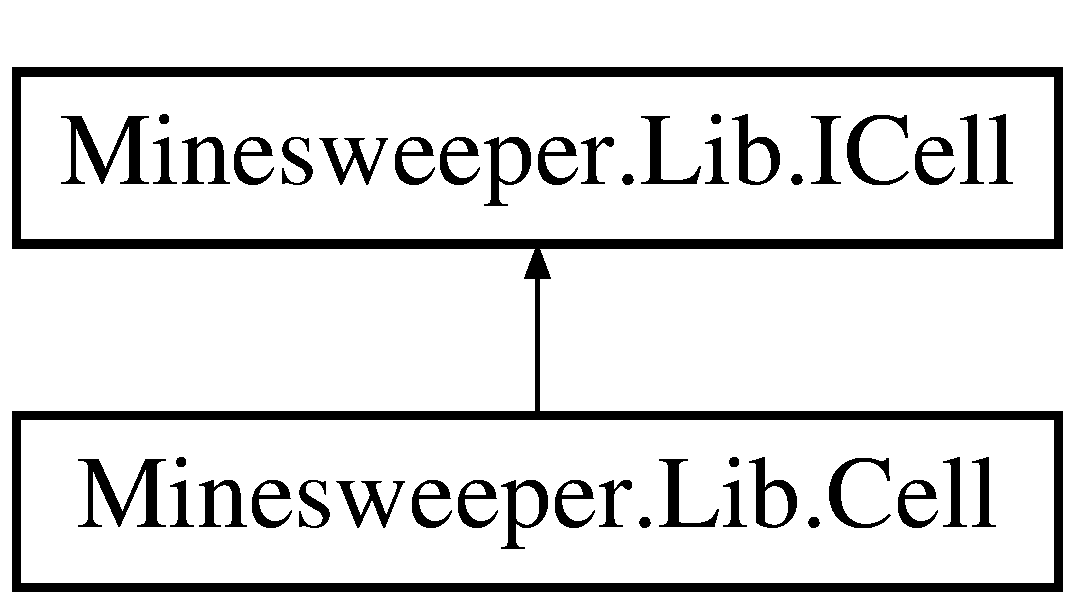
\includegraphics[height=2.000000cm]{interface_minesweeper_1_1_lib_1_1_i_cell}
\end{center}
\end{figure}
\subsection*{Public Member Functions}
\begin{DoxyCompactItemize}
\item 
void \hyperlink{interface_minesweeper_1_1_lib_1_1_i_cell_aa7b5d6db30495f23c0aa595e95aa16ae}{Open\+Cell} ()
\begin{DoxyCompactList}\small\item\em Opens the current cell. \end{DoxyCompactList}\item 
void \hyperlink{interface_minesweeper_1_1_lib_1_1_i_cell_acb11d64a47cb3176d2fe42a093958e49}{Toggle\+Flag} ()
\begin{DoxyCompactList}\small\item\em Toggles the flag of the current cell. \end{DoxyCompactList}\item 
void \hyperlink{interface_minesweeper_1_1_lib_1_1_i_cell_a0befb554376beed982e468052e7c0ed6}{Add\+Mine} ()
\begin{DoxyCompactList}\small\item\em Adds mine to the current cell. \end{DoxyCompactList}\item 
void \hyperlink{interface_minesweeper_1_1_lib_1_1_i_cell_a12556fc759e102491c7ce2c432bd0dec}{Disarm} ()
\begin{DoxyCompactList}\small\item\em Removes a mine from the current cell. \end{DoxyCompactList}\end{DoxyCompactItemize}
\subsection*{Properties}
\begin{DoxyCompactItemize}
\item 
bool \hyperlink{interface_minesweeper_1_1_lib_1_1_i_cell_a02ffb839dc8dc60f261628916e2ac62a}{Is\+Opened}\hspace{0.3cm}{\ttfamily  \mbox{[}get\mbox{]}}
\begin{DoxyCompactList}\small\item\em Gets a value indicating whether the current cell is opened. \end{DoxyCompactList}\item 
bool \hyperlink{interface_minesweeper_1_1_lib_1_1_i_cell_a4bd673766caa3ba4975bcbdc092c61c6}{Is\+Mined}\hspace{0.3cm}{\ttfamily  \mbox{[}get\mbox{]}}
\begin{DoxyCompactList}\small\item\em Gets a value indicating whether the current cell is mined. \end{DoxyCompactList}\item 
bool \hyperlink{interface_minesweeper_1_1_lib_1_1_i_cell_ad854c4d0c51388abb1b11634184ba361}{Is\+Flagged}\hspace{0.3cm}{\ttfamily  \mbox{[}get\mbox{]}}
\begin{DoxyCompactList}\small\item\em Gets a value indicating whether the current cell is flagged. \end{DoxyCompactList}\end{DoxyCompactItemize}


\subsection{Detailed Description}
Defines methods for interacting with a cell. 



\subsection{Member Function Documentation}
\hypertarget{interface_minesweeper_1_1_lib_1_1_i_cell_a0befb554376beed982e468052e7c0ed6}{\index{Minesweeper\+::\+Lib\+::\+I\+Cell@{Minesweeper\+::\+Lib\+::\+I\+Cell}!Add\+Mine@{Add\+Mine}}
\index{Add\+Mine@{Add\+Mine}!Minesweeper\+::\+Lib\+::\+I\+Cell@{Minesweeper\+::\+Lib\+::\+I\+Cell}}
\subsubsection[{Add\+Mine}]{\setlength{\rightskip}{0pt plus 5cm}void Minesweeper.\+Lib.\+I\+Cell.\+Add\+Mine (
\begin{DoxyParamCaption}
{}
\end{DoxyParamCaption}
)}}\label{interface_minesweeper_1_1_lib_1_1_i_cell_a0befb554376beed982e468052e7c0ed6}


Adds mine to the current cell. 



Implemented in \hyperlink{class_minesweeper_1_1_lib_1_1_cell_a64366640c2cb5425cc73817827d291c4}{Minesweeper.\+Lib.\+Cell}.

\hypertarget{interface_minesweeper_1_1_lib_1_1_i_cell_a12556fc759e102491c7ce2c432bd0dec}{\index{Minesweeper\+::\+Lib\+::\+I\+Cell@{Minesweeper\+::\+Lib\+::\+I\+Cell}!Disarm@{Disarm}}
\index{Disarm@{Disarm}!Minesweeper\+::\+Lib\+::\+I\+Cell@{Minesweeper\+::\+Lib\+::\+I\+Cell}}
\subsubsection[{Disarm}]{\setlength{\rightskip}{0pt plus 5cm}void Minesweeper.\+Lib.\+I\+Cell.\+Disarm (
\begin{DoxyParamCaption}
{}
\end{DoxyParamCaption}
)}}\label{interface_minesweeper_1_1_lib_1_1_i_cell_a12556fc759e102491c7ce2c432bd0dec}


Removes a mine from the current cell. 



Implemented in \hyperlink{class_minesweeper_1_1_lib_1_1_cell_ad69f61697ceb611c855f3c4e48f60eb4}{Minesweeper.\+Lib.\+Cell}.

\hypertarget{interface_minesweeper_1_1_lib_1_1_i_cell_aa7b5d6db30495f23c0aa595e95aa16ae}{\index{Minesweeper\+::\+Lib\+::\+I\+Cell@{Minesweeper\+::\+Lib\+::\+I\+Cell}!Open\+Cell@{Open\+Cell}}
\index{Open\+Cell@{Open\+Cell}!Minesweeper\+::\+Lib\+::\+I\+Cell@{Minesweeper\+::\+Lib\+::\+I\+Cell}}
\subsubsection[{Open\+Cell}]{\setlength{\rightskip}{0pt plus 5cm}void Minesweeper.\+Lib.\+I\+Cell.\+Open\+Cell (
\begin{DoxyParamCaption}
{}
\end{DoxyParamCaption}
)}}\label{interface_minesweeper_1_1_lib_1_1_i_cell_aa7b5d6db30495f23c0aa595e95aa16ae}


Opens the current cell. 



Implemented in \hyperlink{class_minesweeper_1_1_lib_1_1_cell_a5fa36c247bd91a482ac46ebf7d2f38b8}{Minesweeper.\+Lib.\+Cell}.

\hypertarget{interface_minesweeper_1_1_lib_1_1_i_cell_acb11d64a47cb3176d2fe42a093958e49}{\index{Minesweeper\+::\+Lib\+::\+I\+Cell@{Minesweeper\+::\+Lib\+::\+I\+Cell}!Toggle\+Flag@{Toggle\+Flag}}
\index{Toggle\+Flag@{Toggle\+Flag}!Minesweeper\+::\+Lib\+::\+I\+Cell@{Minesweeper\+::\+Lib\+::\+I\+Cell}}
\subsubsection[{Toggle\+Flag}]{\setlength{\rightskip}{0pt plus 5cm}void Minesweeper.\+Lib.\+I\+Cell.\+Toggle\+Flag (
\begin{DoxyParamCaption}
{}
\end{DoxyParamCaption}
)}}\label{interface_minesweeper_1_1_lib_1_1_i_cell_acb11d64a47cb3176d2fe42a093958e49}


Toggles the flag of the current cell. 



Implemented in \hyperlink{class_minesweeper_1_1_lib_1_1_cell_a0f959eea2ba69dfa8fcb0ee72e8b33ca}{Minesweeper.\+Lib.\+Cell}.



\subsection{Property Documentation}
\hypertarget{interface_minesweeper_1_1_lib_1_1_i_cell_ad854c4d0c51388abb1b11634184ba361}{\index{Minesweeper\+::\+Lib\+::\+I\+Cell@{Minesweeper\+::\+Lib\+::\+I\+Cell}!Is\+Flagged@{Is\+Flagged}}
\index{Is\+Flagged@{Is\+Flagged}!Minesweeper\+::\+Lib\+::\+I\+Cell@{Minesweeper\+::\+Lib\+::\+I\+Cell}}
\subsubsection[{Is\+Flagged}]{\setlength{\rightskip}{0pt plus 5cm}bool Minesweeper.\+Lib.\+I\+Cell.\+Is\+Flagged\hspace{0.3cm}{\ttfamily [get]}}}\label{interface_minesweeper_1_1_lib_1_1_i_cell_ad854c4d0c51388abb1b11634184ba361}


Gets a value indicating whether the current cell is flagged. 

True if the current cell is flagged.\hypertarget{interface_minesweeper_1_1_lib_1_1_i_cell_a4bd673766caa3ba4975bcbdc092c61c6}{\index{Minesweeper\+::\+Lib\+::\+I\+Cell@{Minesweeper\+::\+Lib\+::\+I\+Cell}!Is\+Mined@{Is\+Mined}}
\index{Is\+Mined@{Is\+Mined}!Minesweeper\+::\+Lib\+::\+I\+Cell@{Minesweeper\+::\+Lib\+::\+I\+Cell}}
\subsubsection[{Is\+Mined}]{\setlength{\rightskip}{0pt plus 5cm}bool Minesweeper.\+Lib.\+I\+Cell.\+Is\+Mined\hspace{0.3cm}{\ttfamily [get]}}}\label{interface_minesweeper_1_1_lib_1_1_i_cell_a4bd673766caa3ba4975bcbdc092c61c6}


Gets a value indicating whether the current cell is mined. 

True if the current cell has a mine.\hypertarget{interface_minesweeper_1_1_lib_1_1_i_cell_a02ffb839dc8dc60f261628916e2ac62a}{\index{Minesweeper\+::\+Lib\+::\+I\+Cell@{Minesweeper\+::\+Lib\+::\+I\+Cell}!Is\+Opened@{Is\+Opened}}
\index{Is\+Opened@{Is\+Opened}!Minesweeper\+::\+Lib\+::\+I\+Cell@{Minesweeper\+::\+Lib\+::\+I\+Cell}}
\subsubsection[{Is\+Opened}]{\setlength{\rightskip}{0pt plus 5cm}bool Minesweeper.\+Lib.\+I\+Cell.\+Is\+Opened\hspace{0.3cm}{\ttfamily [get]}}}\label{interface_minesweeper_1_1_lib_1_1_i_cell_a02ffb839dc8dc60f261628916e2ac62a}


Gets a value indicating whether the current cell is opened. 

True if the current cell is opened.

The documentation for this interface was generated from the following file\+:\begin{DoxyCompactItemize}
\item 
Minesweeper/\+Minesweeper/\+Minesweeper.\+Lib/\+Interfaces/I\+Cell.\+cs\end{DoxyCompactItemize}

\hypertarget{interface_minesweeper_1_1_lib_1_1_i_cell_position}{\section{Minesweeper.\+Lib.\+I\+Cell\+Position Interface Reference}
\label{interface_minesweeper_1_1_lib_1_1_i_cell_position}\index{Minesweeper.\+Lib.\+I\+Cell\+Position@{Minesweeper.\+Lib.\+I\+Cell\+Position}}
}


Defines properties for the cell position.  


Inheritance diagram for Minesweeper.\+Lib.\+I\+Cell\+Position\+:\begin{figure}[H]
\begin{center}
\leavevmode
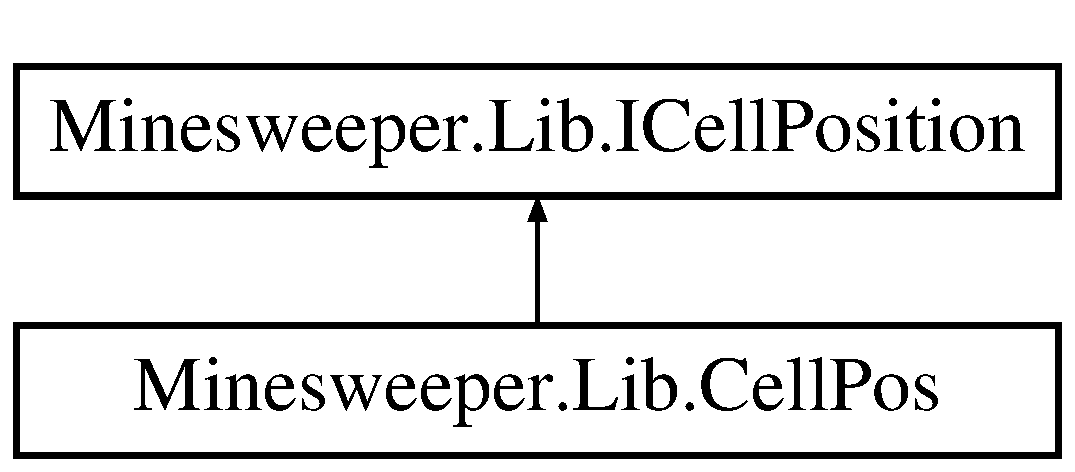
\includegraphics[height=2.000000cm]{interface_minesweeper_1_1_lib_1_1_i_cell_position}
\end{center}
\end{figure}
\subsection*{Properties}
\begin{DoxyCompactItemize}
\item 
int \hyperlink{interface_minesweeper_1_1_lib_1_1_i_cell_position_a41fc9d6cadddc3e5c66d01746f74f823}{Row}\hspace{0.3cm}{\ttfamily  \mbox{[}get, set\mbox{]}}
\begin{DoxyCompactList}\small\item\em Gets or sets value for position by row. \end{DoxyCompactList}\item 
int \hyperlink{interface_minesweeper_1_1_lib_1_1_i_cell_position_aca8beb37824e81653e0b2425a2dd475e}{Col}\hspace{0.3cm}{\ttfamily  \mbox{[}get, set\mbox{]}}
\begin{DoxyCompactList}\small\item\em Gets or sets value for position by column. \end{DoxyCompactList}\end{DoxyCompactItemize}


\subsection{Detailed Description}
Defines properties for the cell position. 



\subsection{Property Documentation}
\hypertarget{interface_minesweeper_1_1_lib_1_1_i_cell_position_aca8beb37824e81653e0b2425a2dd475e}{\index{Minesweeper\+::\+Lib\+::\+I\+Cell\+Position@{Minesweeper\+::\+Lib\+::\+I\+Cell\+Position}!Col@{Col}}
\index{Col@{Col}!Minesweeper\+::\+Lib\+::\+I\+Cell\+Position@{Minesweeper\+::\+Lib\+::\+I\+Cell\+Position}}
\subsubsection[{Col}]{\setlength{\rightskip}{0pt plus 5cm}int Minesweeper.\+Lib.\+I\+Cell\+Position.\+Col\hspace{0.3cm}{\ttfamily [get]}, {\ttfamily [set]}}}\label{interface_minesweeper_1_1_lib_1_1_i_cell_position_aca8beb37824e81653e0b2425a2dd475e}


Gets or sets value for position by column. 

Position by column.\hypertarget{interface_minesweeper_1_1_lib_1_1_i_cell_position_a41fc9d6cadddc3e5c66d01746f74f823}{\index{Minesweeper\+::\+Lib\+::\+I\+Cell\+Position@{Minesweeper\+::\+Lib\+::\+I\+Cell\+Position}!Row@{Row}}
\index{Row@{Row}!Minesweeper\+::\+Lib\+::\+I\+Cell\+Position@{Minesweeper\+::\+Lib\+::\+I\+Cell\+Position}}
\subsubsection[{Row}]{\setlength{\rightskip}{0pt plus 5cm}int Minesweeper.\+Lib.\+I\+Cell\+Position.\+Row\hspace{0.3cm}{\ttfamily [get]}, {\ttfamily [set]}}}\label{interface_minesweeper_1_1_lib_1_1_i_cell_position_a41fc9d6cadddc3e5c66d01746f74f823}


Gets or sets value for position by row. 

Position by row.

The documentation for this interface was generated from the following file\+:\begin{DoxyCompactItemize}
\item 
Minesweeper/\+Minesweeper/\+Minesweeper.\+Lib/\+Interfaces/I\+Cell\+Position.\+cs\end{DoxyCompactItemize}

\hypertarget{interface_minesweeper_1_1_game_1_1_i_command}{\section{Minesweeper.\+Game.\+I\+Command Interface Reference}
\label{interface_minesweeper_1_1_game_1_1_i_command}\index{Minesweeper.\+Game.\+I\+Command@{Minesweeper.\+Game.\+I\+Command}}
}


The 'Command' interface.  


Inheritance diagram for Minesweeper.\+Game.\+I\+Command\+:\begin{figure}[H]
\begin{center}
\leavevmode
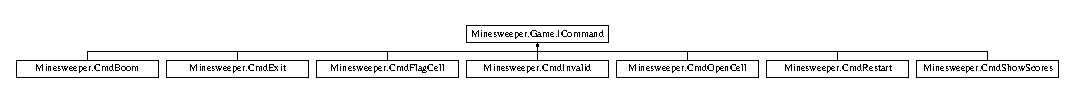
\includegraphics[height=0.816327cm]{interface_minesweeper_1_1_game_1_1_i_command}
\end{center}
\end{figure}
\subsection*{Public Member Functions}
\begin{DoxyCompactItemize}
\item 
bool \hyperlink{interface_minesweeper_1_1_game_1_1_i_command_a03482e68480cad46a8cf419a87440cc9}{Execute} ()
\begin{DoxyCompactList}\small\item\em Invokes the action on the needed object. \end{DoxyCompactList}\end{DoxyCompactItemize}


\subsection{Detailed Description}
The 'Command' interface. 



\subsection{Member Function Documentation}
\hypertarget{interface_minesweeper_1_1_game_1_1_i_command_a03482e68480cad46a8cf419a87440cc9}{\index{Minesweeper\+::\+Game\+::\+I\+Command@{Minesweeper\+::\+Game\+::\+I\+Command}!Execute@{Execute}}
\index{Execute@{Execute}!Minesweeper\+::\+Game\+::\+I\+Command@{Minesweeper\+::\+Game\+::\+I\+Command}}
\subsubsection[{Execute}]{\setlength{\rightskip}{0pt plus 5cm}bool Minesweeper.\+Game.\+I\+Command.\+Execute (
\begin{DoxyParamCaption}
{}
\end{DoxyParamCaption}
)}}\label{interface_minesweeper_1_1_game_1_1_i_command_a03482e68480cad46a8cf419a87440cc9}


Invokes the action on the needed object. 

\begin{DoxyReturn}{Returns}
Returns true if more commands can be executed.
\end{DoxyReturn}


Implemented in \hyperlink{class_minesweeper_1_1_cmd_flag_cell_ab8fdee19beed086308829c7d3ae9b7ef}{Minesweeper.\+Cmd\+Flag\+Cell}, \hyperlink{class_minesweeper_1_1_cmd_open_cell_ad8627666ebddf09daf909b3c66173954}{Minesweeper.\+Cmd\+Open\+Cell}, \hyperlink{class_minesweeper_1_1_cmd_boom_ac98aceae68a835b332342321a1a53abe}{Minesweeper.\+Cmd\+Boom}, \hyperlink{class_minesweeper_1_1_cmd_exit_a218e1498a94ac5b49f0dab48d4f154aa}{Minesweeper.\+Cmd\+Exit}, \hyperlink{class_minesweeper_1_1_cmd_invalid_a7d6834d857c3159a20160c2eb94c557e}{Minesweeper.\+Cmd\+Invalid}, \hyperlink{class_minesweeper_1_1_cmd_restart_a58ff1eea35e4a710c840eedcd421122f}{Minesweeper.\+Cmd\+Restart}, and \hyperlink{class_minesweeper_1_1_cmd_show_scores_ab704f1d09e8802999384c6af9d8d807b}{Minesweeper.\+Cmd\+Show\+Scores}.



The documentation for this interface was generated from the following file\+:\begin{DoxyCompactItemize}
\item 
Minesweeper/\+Minesweeper/\+Minesweeper.\+game/I\+Command.\+cs\end{DoxyCompactItemize}

\hypertarget{interface_minesweeper_1_1_lib_1_1_i_random_generator_provider}{\section{Minesweeper.\+Lib.\+I\+Random\+Generator\+Provider Interface Reference}
\label{interface_minesweeper_1_1_lib_1_1_i_random_generator_provider}\index{Minesweeper.\+Lib.\+I\+Random\+Generator\+Provider@{Minesweeper.\+Lib.\+I\+Random\+Generator\+Provider}}
}


Random number provider interface.  


Inheritance diagram for Minesweeper.\+Lib.\+I\+Random\+Generator\+Provider\+:\begin{figure}[H]
\begin{center}
\leavevmode
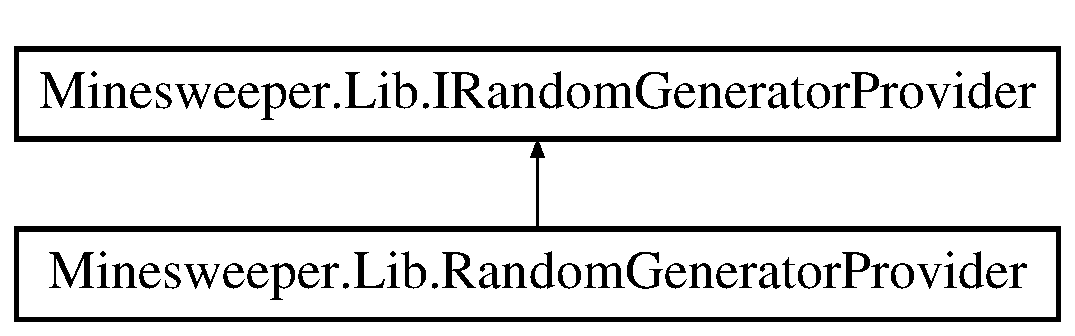
\includegraphics[height=2.000000cm]{interface_minesweeper_1_1_lib_1_1_i_random_generator_provider}
\end{center}
\end{figure}
\subsection*{Public Member Functions}
\begin{DoxyCompactItemize}
\item 
int \hyperlink{interface_minesweeper_1_1_lib_1_1_i_random_generator_provider_a0f49fa42c327f257a83bfb9264cb9124}{Next} (int min, int max)
\begin{DoxyCompactList}\small\item\em Generates random number in range. \end{DoxyCompactList}\item 
int \hyperlink{interface_minesweeper_1_1_lib_1_1_i_random_generator_provider_a582bbebd6de2ecdded37c76b35c74a66}{Next} (int max)
\begin{DoxyCompactList}\small\item\em Overload with min range 0. \end{DoxyCompactList}\end{DoxyCompactItemize}


\subsection{Detailed Description}
Random number provider interface. 



\subsection{Member Function Documentation}
\hypertarget{interface_minesweeper_1_1_lib_1_1_i_random_generator_provider_a0f49fa42c327f257a83bfb9264cb9124}{\index{Minesweeper\+::\+Lib\+::\+I\+Random\+Generator\+Provider@{Minesweeper\+::\+Lib\+::\+I\+Random\+Generator\+Provider}!Next@{Next}}
\index{Next@{Next}!Minesweeper\+::\+Lib\+::\+I\+Random\+Generator\+Provider@{Minesweeper\+::\+Lib\+::\+I\+Random\+Generator\+Provider}}
\subsubsection[{Next}]{\setlength{\rightskip}{0pt plus 5cm}int Minesweeper.\+Lib.\+I\+Random\+Generator\+Provider.\+Next (
\begin{DoxyParamCaption}
\item[{int}]{min, }
\item[{int}]{max}
\end{DoxyParamCaption}
)}}\label{interface_minesweeper_1_1_lib_1_1_i_random_generator_provider_a0f49fa42c327f257a83bfb9264cb9124}


Generates random number in range. 


\begin{DoxyParams}{Parameters}
{\em min} & Minimal range.\\
\hline
{\em max} & Maximal range.\\
\hline
\end{DoxyParams}
\begin{DoxyReturn}{Returns}
Random integer number.
\end{DoxyReturn}


Implemented in \hyperlink{class_minesweeper_1_1_lib_1_1_random_generator_provider_a53e1e507758a05548dd09e14c81af8d4}{Minesweeper.\+Lib.\+Random\+Generator\+Provider}.

\hypertarget{interface_minesweeper_1_1_lib_1_1_i_random_generator_provider_a582bbebd6de2ecdded37c76b35c74a66}{\index{Minesweeper\+::\+Lib\+::\+I\+Random\+Generator\+Provider@{Minesweeper\+::\+Lib\+::\+I\+Random\+Generator\+Provider}!Next@{Next}}
\index{Next@{Next}!Minesweeper\+::\+Lib\+::\+I\+Random\+Generator\+Provider@{Minesweeper\+::\+Lib\+::\+I\+Random\+Generator\+Provider}}
\subsubsection[{Next}]{\setlength{\rightskip}{0pt plus 5cm}int Minesweeper.\+Lib.\+I\+Random\+Generator\+Provider.\+Next (
\begin{DoxyParamCaption}
\item[{int}]{max}
\end{DoxyParamCaption}
)}}\label{interface_minesweeper_1_1_lib_1_1_i_random_generator_provider_a582bbebd6de2ecdded37c76b35c74a66}


Overload with min range 0. 


\begin{DoxyParams}{Parameters}
{\em max} & Maximal range.\\
\hline
\end{DoxyParams}
\begin{DoxyReturn}{Returns}
Random integer number.
\end{DoxyReturn}


Implemented in \hyperlink{class_minesweeper_1_1_lib_1_1_random_generator_provider_afabb9a038955a531abcb19cb0c6b77a3}{Minesweeper.\+Lib.\+Random\+Generator\+Provider}.



The documentation for this interface was generated from the following file\+:\begin{DoxyCompactItemize}
\item 
Minesweeper/\+Minesweeper/\+Minesweeper.\+Lib/\+Interfaces/I\+Random\+Generator\+Provider.\+cs\end{DoxyCompactItemize}

\hypertarget{interface_minesweeper_1_1_lib_1_1_i_renderer}{\section{Minesweeper.\+Lib.\+I\+Renderer Interface Reference}
\label{interface_minesweeper_1_1_lib_1_1_i_renderer}\index{Minesweeper.\+Lib.\+I\+Renderer@{Minesweeper.\+Lib.\+I\+Renderer}}
}


Defines methods for rendering text.  


Inheritance diagram for Minesweeper.\+Lib.\+I\+Renderer\+:\begin{figure}[H]
\begin{center}
\leavevmode
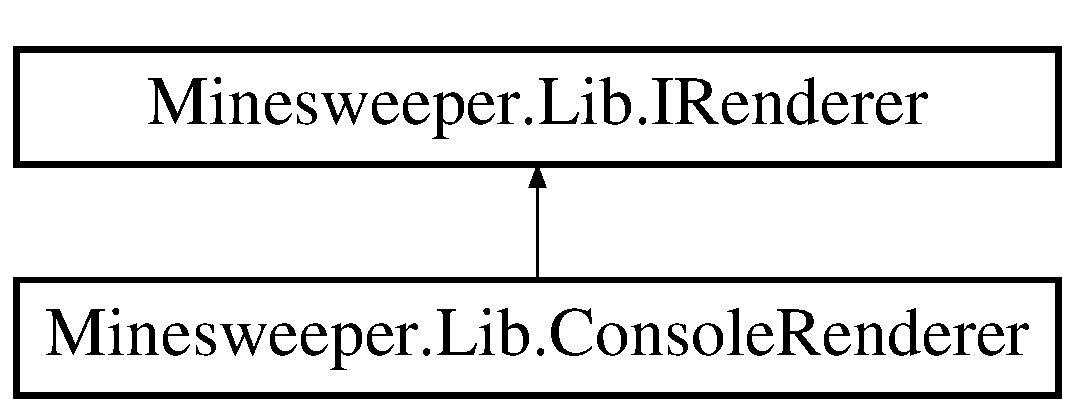
\includegraphics[height=2.000000cm]{interface_minesweeper_1_1_lib_1_1_i_renderer}
\end{center}
\end{figure}
\subsection*{Public Member Functions}
\begin{DoxyCompactItemize}
\item 
void \hyperlink{interface_minesweeper_1_1_lib_1_1_i_renderer_a150b8784f5e36e60321bde94eee5547d}{Write\+Line} ()
\begin{DoxyCompactList}\small\item\em Writes the current line terminator to the output stream. \end{DoxyCompactList}\item 
void \hyperlink{interface_minesweeper_1_1_lib_1_1_i_renderer_a70b1435fe82e94c6b97367b374b70d05}{Write\+Line} (string format, params object\mbox{[}$\,$\mbox{]} args)
\begin{DoxyCompactList}\small\item\em Writes the text representation of the specified array of objects to the output stream using the specified format information, followed by the current line terminator. \end{DoxyCompactList}\item 
void \hyperlink{interface_minesweeper_1_1_lib_1_1_i_renderer_a05ea2257710476341378ee29f6f7762b}{Write} (string format, params object\mbox{[}$\,$\mbox{]} args)
\begin{DoxyCompactList}\small\item\em Writes the text representation of the specified array of objects to the output stream using the specified format information. \end{DoxyCompactList}\item 
void \hyperlink{interface_minesweeper_1_1_lib_1_1_i_renderer_a1f08c5c282e4ce3d59f0e6734c90bdf7}{Write\+At} (int left, int top, string format, params object\mbox{[}$\,$\mbox{]} args)
\begin{DoxyCompactList}\small\item\em Writes the text representation of the specified array of objects to the output stream using the specified format information at a specific position. \end{DoxyCompactList}\item 
void \hyperlink{interface_minesweeper_1_1_lib_1_1_i_renderer_ab9daae4f93263816808f642cba7e9875}{Clear\+Lines} (int left, int top, int num\+Lines)
\begin{DoxyCompactList}\small\item\em Clear specific number of lines. \end{DoxyCompactList}\end{DoxyCompactItemize}


\subsection{Detailed Description}
Defines methods for rendering text. 



\subsection{Member Function Documentation}
\hypertarget{interface_minesweeper_1_1_lib_1_1_i_renderer_ab9daae4f93263816808f642cba7e9875}{\index{Minesweeper\+::\+Lib\+::\+I\+Renderer@{Minesweeper\+::\+Lib\+::\+I\+Renderer}!Clear\+Lines@{Clear\+Lines}}
\index{Clear\+Lines@{Clear\+Lines}!Minesweeper\+::\+Lib\+::\+I\+Renderer@{Minesweeper\+::\+Lib\+::\+I\+Renderer}}
\subsubsection[{Clear\+Lines}]{\setlength{\rightskip}{0pt plus 5cm}void Minesweeper.\+Lib.\+I\+Renderer.\+Clear\+Lines (
\begin{DoxyParamCaption}
\item[{int}]{left, }
\item[{int}]{top, }
\item[{int}]{num\+Lines}
\end{DoxyParamCaption}
)}}\label{interface_minesweeper_1_1_lib_1_1_i_renderer_ab9daae4f93263816808f642cba7e9875}


Clear specific number of lines. 


\begin{DoxyParams}{Parameters}
{\em left} & Start column position of the clearing.\\
\hline
{\em top} & Start row position of the clearing.\\
\hline
{\em num\+Lines} & Number of lines that must be cleared.\\
\hline
\end{DoxyParams}


Implemented in \hyperlink{class_minesweeper_1_1_lib_1_1_console_renderer_a4968ccf049f1704753728368a2519fe2}{Minesweeper.\+Lib.\+Console\+Renderer}.

\hypertarget{interface_minesweeper_1_1_lib_1_1_i_renderer_a05ea2257710476341378ee29f6f7762b}{\index{Minesweeper\+::\+Lib\+::\+I\+Renderer@{Minesweeper\+::\+Lib\+::\+I\+Renderer}!Write@{Write}}
\index{Write@{Write}!Minesweeper\+::\+Lib\+::\+I\+Renderer@{Minesweeper\+::\+Lib\+::\+I\+Renderer}}
\subsubsection[{Write}]{\setlength{\rightskip}{0pt plus 5cm}void Minesweeper.\+Lib.\+I\+Renderer.\+Write (
\begin{DoxyParamCaption}
\item[{string}]{format, }
\item[{params object\mbox{[}$\,$\mbox{]}}]{args}
\end{DoxyParamCaption}
)}}\label{interface_minesweeper_1_1_lib_1_1_i_renderer_a05ea2257710476341378ee29f6f7762b}


Writes the text representation of the specified array of objects to the output stream using the specified format information. 


\begin{DoxyParams}{Parameters}
{\em format} & A composite format string.\\
\hline
{\em args} & An array of objects to write using format.\\
\hline
\end{DoxyParams}


Implemented in \hyperlink{class_minesweeper_1_1_lib_1_1_console_renderer_a14f9db3445bb4f3921eada8463617e35}{Minesweeper.\+Lib.\+Console\+Renderer}.

\hypertarget{interface_minesweeper_1_1_lib_1_1_i_renderer_a1f08c5c282e4ce3d59f0e6734c90bdf7}{\index{Minesweeper\+::\+Lib\+::\+I\+Renderer@{Minesweeper\+::\+Lib\+::\+I\+Renderer}!Write\+At@{Write\+At}}
\index{Write\+At@{Write\+At}!Minesweeper\+::\+Lib\+::\+I\+Renderer@{Minesweeper\+::\+Lib\+::\+I\+Renderer}}
\subsubsection[{Write\+At}]{\setlength{\rightskip}{0pt plus 5cm}void Minesweeper.\+Lib.\+I\+Renderer.\+Write\+At (
\begin{DoxyParamCaption}
\item[{int}]{left, }
\item[{int}]{top, }
\item[{string}]{format, }
\item[{params object\mbox{[}$\,$\mbox{]}}]{args}
\end{DoxyParamCaption}
)}}\label{interface_minesweeper_1_1_lib_1_1_i_renderer_a1f08c5c282e4ce3d59f0e6734c90bdf7}


Writes the text representation of the specified array of objects to the output stream using the specified format information at a specific position. 


\begin{DoxyParams}{Parameters}
{\em left} & The column position.\\
\hline
{\em top} & The row position.\\
\hline
{\em format} & A composite format string.\\
\hline
{\em args} & An array of objects to write using format.\\
\hline
\end{DoxyParams}


Implemented in \hyperlink{class_minesweeper_1_1_lib_1_1_console_renderer_aa8ccd90c8c5a4e6bb02da7b546ef9c26}{Minesweeper.\+Lib.\+Console\+Renderer}.

\hypertarget{interface_minesweeper_1_1_lib_1_1_i_renderer_a150b8784f5e36e60321bde94eee5547d}{\index{Minesweeper\+::\+Lib\+::\+I\+Renderer@{Minesweeper\+::\+Lib\+::\+I\+Renderer}!Write\+Line@{Write\+Line}}
\index{Write\+Line@{Write\+Line}!Minesweeper\+::\+Lib\+::\+I\+Renderer@{Minesweeper\+::\+Lib\+::\+I\+Renderer}}
\subsubsection[{Write\+Line}]{\setlength{\rightskip}{0pt plus 5cm}void Minesweeper.\+Lib.\+I\+Renderer.\+Write\+Line (
\begin{DoxyParamCaption}
{}
\end{DoxyParamCaption}
)}}\label{interface_minesweeper_1_1_lib_1_1_i_renderer_a150b8784f5e36e60321bde94eee5547d}


Writes the current line terminator to the output stream. 



Implemented in \hyperlink{class_minesweeper_1_1_lib_1_1_console_renderer_a0a9b86365042b44de6c5b9da7b40dafe}{Minesweeper.\+Lib.\+Console\+Renderer}.

\hypertarget{interface_minesweeper_1_1_lib_1_1_i_renderer_a70b1435fe82e94c6b97367b374b70d05}{\index{Minesweeper\+::\+Lib\+::\+I\+Renderer@{Minesweeper\+::\+Lib\+::\+I\+Renderer}!Write\+Line@{Write\+Line}}
\index{Write\+Line@{Write\+Line}!Minesweeper\+::\+Lib\+::\+I\+Renderer@{Minesweeper\+::\+Lib\+::\+I\+Renderer}}
\subsubsection[{Write\+Line}]{\setlength{\rightskip}{0pt plus 5cm}void Minesweeper.\+Lib.\+I\+Renderer.\+Write\+Line (
\begin{DoxyParamCaption}
\item[{string}]{format, }
\item[{params object\mbox{[}$\,$\mbox{]}}]{args}
\end{DoxyParamCaption}
)}}\label{interface_minesweeper_1_1_lib_1_1_i_renderer_a70b1435fe82e94c6b97367b374b70d05}


Writes the text representation of the specified array of objects to the output stream using the specified format information, followed by the current line terminator. 


\begin{DoxyParams}{Parameters}
{\em format} & A composite format string.\\
\hline
{\em args} & An array of objects to write using format.\\
\hline
\end{DoxyParams}


Implemented in \hyperlink{class_minesweeper_1_1_lib_1_1_console_renderer_afe92f94092a0a7876ec1c845ee7d78cf}{Minesweeper.\+Lib.\+Console\+Renderer}.



The documentation for this interface was generated from the following file\+:\begin{DoxyCompactItemize}
\item 
Minesweeper/\+Minesweeper/\+Minesweeper.\+Lib/\+Interfaces/I\+Renderer.\+cs\end{DoxyCompactItemize}

\hypertarget{interface_minesweeper_1_1_game_1_1_i_u_i_manager}{\section{Minesweeper.\+Game.\+I\+U\+I\+Manager Interface Reference}
\label{interface_minesweeper_1_1_game_1_1_i_u_i_manager}\index{Minesweeper.\+Game.\+I\+U\+I\+Manager@{Minesweeper.\+Game.\+I\+U\+I\+Manager}}
}


Defines methods for reading and writing.  


Inheritance diagram for Minesweeper.\+Game.\+I\+U\+I\+Manager\+:\begin{figure}[H]
\begin{center}
\leavevmode
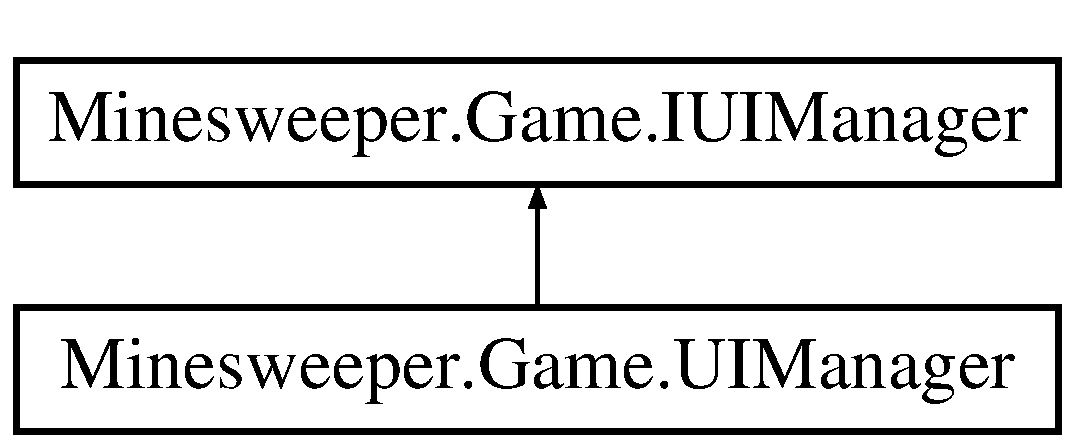
\includegraphics[height=2.000000cm]{interface_minesweeper_1_1_game_1_1_i_u_i_manager}
\end{center}
\end{figure}
\subsection*{Public Member Functions}
\begin{DoxyCompactItemize}
\item 
void \hyperlink{interface_minesweeper_1_1_game_1_1_i_u_i_manager_aafbe4485c18fe5dd0269a1a54599d1fc}{Clear\+Command\+Line} (string command\+Prompt)
\begin{DoxyCompactList}\small\item\em Clears the command line. \end{DoxyCompactList}\item 
void \hyperlink{interface_minesweeper_1_1_game_1_1_i_u_i_manager_a7df49d712d01db2b9e9b36218667cc23}{Display\+End} (string msg, int number\+Of\+Opened\+Cells)
\begin{DoxyCompactList}\small\item\em Displays the ending messages of the game. \end{DoxyCompactList}\item 
void \hyperlink{interface_minesweeper_1_1_game_1_1_i_u_i_manager_afa8d49b68057b38c302d945c829e1856}{Display\+Error} (string error\+Msg)
\begin{DoxyCompactList}\small\item\em Displays error messages. \end{DoxyCompactList}\item 
void \hyperlink{interface_minesweeper_1_1_game_1_1_i_u_i_manager_a562c29c1904a923494c26511e0a6a3d8}{Display\+High\+Scores} (I\+Enumerable$<$ Key\+Value\+Pair$<$ string, int $>$$>$ top\+Scores)
\begin{DoxyCompactList}\small\item\em Displays the high scores. \end{DoxyCompactList}\item 
void \hyperlink{interface_minesweeper_1_1_game_1_1_i_u_i_manager_a0a8ff25e5b1a5013bdbf2c5b7a5f82c3}{Display\+Intro} (string msg)
\begin{DoxyCompactList}\small\item\em Displays the introduction text of the game. \end{DoxyCompactList}\item 
void \hyperlink{interface_minesweeper_1_1_game_1_1_i_u_i_manager_acae1778c1bdc80065c2b18afb1d11a70}{Draw\+Game\+Field} (\hyperlink{namespace_minesweeper_adf92d608047dafd69d16008492d317bd}{Cell\+Image}\mbox{[},\mbox{]} minefield, int\mbox{[},\mbox{]} neighbor\+Mines)
\begin{DoxyCompactList}\small\item\em Draws the game field. \end{DoxyCompactList}\item 
void \hyperlink{interface_minesweeper_1_1_game_1_1_i_u_i_manager_a0dd9d9e47eba3707562cf1493a9bf6aa}{Draw\+Table} (int mine\+Field\+Rows, int minefield\+Cols)
\begin{DoxyCompactList}\small\item\em Draws the game table. \end{DoxyCompactList}\item 
void \hyperlink{interface_minesweeper_1_1_game_1_1_i_u_i_manager_a61f1153446f2f52f258363ccd9008c20}{Good\+Bye} (string good\+Bye\+Msg)
\begin{DoxyCompactList}\small\item\em Displays the messages when the user quits the game. \end{DoxyCompactList}\item 
string \hyperlink{interface_minesweeper_1_1_game_1_1_i_u_i_manager_ac2d51aed7d1d677c899fa596becc6afb}{Read\+Input} ()
\begin{DoxyCompactList}\small\item\em Reads input from the user. \end{DoxyCompactList}\end{DoxyCompactItemize}


\subsection{Detailed Description}
Defines methods for reading and writing. 



\subsection{Member Function Documentation}
\hypertarget{interface_minesweeper_1_1_game_1_1_i_u_i_manager_aafbe4485c18fe5dd0269a1a54599d1fc}{\index{Minesweeper\+::\+Game\+::\+I\+U\+I\+Manager@{Minesweeper\+::\+Game\+::\+I\+U\+I\+Manager}!Clear\+Command\+Line@{Clear\+Command\+Line}}
\index{Clear\+Command\+Line@{Clear\+Command\+Line}!Minesweeper\+::\+Game\+::\+I\+U\+I\+Manager@{Minesweeper\+::\+Game\+::\+I\+U\+I\+Manager}}
\subsubsection[{Clear\+Command\+Line}]{\setlength{\rightskip}{0pt plus 5cm}void Minesweeper.\+Game.\+I\+U\+I\+Manager.\+Clear\+Command\+Line (
\begin{DoxyParamCaption}
\item[{string}]{command\+Prompt}
\end{DoxyParamCaption}
)}}\label{interface_minesweeper_1_1_game_1_1_i_u_i_manager_aafbe4485c18fe5dd0269a1a54599d1fc}


Clears the command line. 


\begin{DoxyParams}{Parameters}
{\em command\+Prompt} & The prompt that is going to be shown to the user.\\
\hline
\end{DoxyParams}


Implemented in \hyperlink{class_minesweeper_1_1_game_1_1_u_i_manager_acc84e19d875400108a4026cf2861c5d9}{Minesweeper.\+Game.\+U\+I\+Manager}.

\hypertarget{interface_minesweeper_1_1_game_1_1_i_u_i_manager_a7df49d712d01db2b9e9b36218667cc23}{\index{Minesweeper\+::\+Game\+::\+I\+U\+I\+Manager@{Minesweeper\+::\+Game\+::\+I\+U\+I\+Manager}!Display\+End@{Display\+End}}
\index{Display\+End@{Display\+End}!Minesweeper\+::\+Game\+::\+I\+U\+I\+Manager@{Minesweeper\+::\+Game\+::\+I\+U\+I\+Manager}}
\subsubsection[{Display\+End}]{\setlength{\rightskip}{0pt plus 5cm}void Minesweeper.\+Game.\+I\+U\+I\+Manager.\+Display\+End (
\begin{DoxyParamCaption}
\item[{string}]{msg, }
\item[{int}]{number\+Of\+Opened\+Cells}
\end{DoxyParamCaption}
)}}\label{interface_minesweeper_1_1_game_1_1_i_u_i_manager_a7df49d712d01db2b9e9b36218667cc23}


Displays the ending messages of the game. 


\begin{DoxyParams}{Parameters}
{\em msg} & The ending message.\\
\hline
{\em number\+Of\+Opened\+Cells} & The number of cells the user opened during the game.\\
\hline
\end{DoxyParams}


Implemented in \hyperlink{class_minesweeper_1_1_game_1_1_u_i_manager_a32460cc4c19947d1b2f0724a11c1d47c}{Minesweeper.\+Game.\+U\+I\+Manager}.

\hypertarget{interface_minesweeper_1_1_game_1_1_i_u_i_manager_afa8d49b68057b38c302d945c829e1856}{\index{Minesweeper\+::\+Game\+::\+I\+U\+I\+Manager@{Minesweeper\+::\+Game\+::\+I\+U\+I\+Manager}!Display\+Error@{Display\+Error}}
\index{Display\+Error@{Display\+Error}!Minesweeper\+::\+Game\+::\+I\+U\+I\+Manager@{Minesweeper\+::\+Game\+::\+I\+U\+I\+Manager}}
\subsubsection[{Display\+Error}]{\setlength{\rightskip}{0pt plus 5cm}void Minesweeper.\+Game.\+I\+U\+I\+Manager.\+Display\+Error (
\begin{DoxyParamCaption}
\item[{string}]{error\+Msg}
\end{DoxyParamCaption}
)}}\label{interface_minesweeper_1_1_game_1_1_i_u_i_manager_afa8d49b68057b38c302d945c829e1856}


Displays error messages. 


\begin{DoxyParams}{Parameters}
{\em error\+Msg} & The error message to be displayed.\\
\hline
\end{DoxyParams}


Implemented in \hyperlink{class_minesweeper_1_1_game_1_1_u_i_manager_a67f57db959d9eff2829e1c3c64fb726f}{Minesweeper.\+Game.\+U\+I\+Manager}.

\hypertarget{interface_minesweeper_1_1_game_1_1_i_u_i_manager_a562c29c1904a923494c26511e0a6a3d8}{\index{Minesweeper\+::\+Game\+::\+I\+U\+I\+Manager@{Minesweeper\+::\+Game\+::\+I\+U\+I\+Manager}!Display\+High\+Scores@{Display\+High\+Scores}}
\index{Display\+High\+Scores@{Display\+High\+Scores}!Minesweeper\+::\+Game\+::\+I\+U\+I\+Manager@{Minesweeper\+::\+Game\+::\+I\+U\+I\+Manager}}
\subsubsection[{Display\+High\+Scores}]{\setlength{\rightskip}{0pt plus 5cm}void Minesweeper.\+Game.\+I\+U\+I\+Manager.\+Display\+High\+Scores (
\begin{DoxyParamCaption}
\item[{I\+Enumerable$<$ Key\+Value\+Pair$<$ string, int $>$$>$}]{top\+Scores}
\end{DoxyParamCaption}
)}}\label{interface_minesweeper_1_1_game_1_1_i_u_i_manager_a562c29c1904a923494c26511e0a6a3d8}


Displays the high scores. 


\begin{DoxyParams}{Parameters}
{\em top\+Scores} & The top scores to be displayed.\\
\hline
\end{DoxyParams}


Implemented in \hyperlink{class_minesweeper_1_1_game_1_1_u_i_manager_a2f3537e693d8efc90cbef90a0a63d34b}{Minesweeper.\+Game.\+U\+I\+Manager}.

\hypertarget{interface_minesweeper_1_1_game_1_1_i_u_i_manager_a0a8ff25e5b1a5013bdbf2c5b7a5f82c3}{\index{Minesweeper\+::\+Game\+::\+I\+U\+I\+Manager@{Minesweeper\+::\+Game\+::\+I\+U\+I\+Manager}!Display\+Intro@{Display\+Intro}}
\index{Display\+Intro@{Display\+Intro}!Minesweeper\+::\+Game\+::\+I\+U\+I\+Manager@{Minesweeper\+::\+Game\+::\+I\+U\+I\+Manager}}
\subsubsection[{Display\+Intro}]{\setlength{\rightskip}{0pt plus 5cm}void Minesweeper.\+Game.\+I\+U\+I\+Manager.\+Display\+Intro (
\begin{DoxyParamCaption}
\item[{string}]{msg}
\end{DoxyParamCaption}
)}}\label{interface_minesweeper_1_1_game_1_1_i_u_i_manager_a0a8ff25e5b1a5013bdbf2c5b7a5f82c3}


Displays the introduction text of the game. 


\begin{DoxyParams}{Parameters}
{\em msg} & The introduction message.\\
\hline
\end{DoxyParams}


Implemented in \hyperlink{class_minesweeper_1_1_game_1_1_u_i_manager_a854a5ddce1304981c194c0a98d1d9f8c}{Minesweeper.\+Game.\+U\+I\+Manager}.

\hypertarget{interface_minesweeper_1_1_game_1_1_i_u_i_manager_acae1778c1bdc80065c2b18afb1d11a70}{\index{Minesweeper\+::\+Game\+::\+I\+U\+I\+Manager@{Minesweeper\+::\+Game\+::\+I\+U\+I\+Manager}!Draw\+Game\+Field@{Draw\+Game\+Field}}
\index{Draw\+Game\+Field@{Draw\+Game\+Field}!Minesweeper\+::\+Game\+::\+I\+U\+I\+Manager@{Minesweeper\+::\+Game\+::\+I\+U\+I\+Manager}}
\subsubsection[{Draw\+Game\+Field}]{\setlength{\rightskip}{0pt plus 5cm}void Minesweeper.\+Game.\+I\+U\+I\+Manager.\+Draw\+Game\+Field (
\begin{DoxyParamCaption}
\item[{{\bf Cell\+Image}}]{minefield\mbox{[},\mbox{]}, }
\item[{int}]{neighbor\+Mines\mbox{[},\mbox{]}}
\end{DoxyParamCaption}
)}}\label{interface_minesweeper_1_1_game_1_1_i_u_i_manager_acae1778c1bdc80065c2b18afb1d11a70}


Draws the game field. 


\begin{DoxyParams}{Parameters}
{\em minefield} & The minefield to be drawn.\\
\hline
{\em neighbor\+Mines} & The minefield with all values of neighboring mines.\\
\hline
\end{DoxyParams}


Implemented in \hyperlink{class_minesweeper_1_1_game_1_1_u_i_manager_af1af79047deb6ba4ec6902a481df1c3e}{Minesweeper.\+Game.\+U\+I\+Manager}.

\hypertarget{interface_minesweeper_1_1_game_1_1_i_u_i_manager_a0dd9d9e47eba3707562cf1493a9bf6aa}{\index{Minesweeper\+::\+Game\+::\+I\+U\+I\+Manager@{Minesweeper\+::\+Game\+::\+I\+U\+I\+Manager}!Draw\+Table@{Draw\+Table}}
\index{Draw\+Table@{Draw\+Table}!Minesweeper\+::\+Game\+::\+I\+U\+I\+Manager@{Minesweeper\+::\+Game\+::\+I\+U\+I\+Manager}}
\subsubsection[{Draw\+Table}]{\setlength{\rightskip}{0pt plus 5cm}void Minesweeper.\+Game.\+I\+U\+I\+Manager.\+Draw\+Table (
\begin{DoxyParamCaption}
\item[{int}]{mine\+Field\+Rows, }
\item[{int}]{minefield\+Cols}
\end{DoxyParamCaption}
)}}\label{interface_minesweeper_1_1_game_1_1_i_u_i_manager_a0dd9d9e47eba3707562cf1493a9bf6aa}


Draws the game table. 


\begin{DoxyParams}{Parameters}
{\em mine\+Field\+Rows} & The count of the minefield rows.\\
\hline
{\em minefield\+Cols} & The count of the minefield columns.\\
\hline
\end{DoxyParams}


Implemented in \hyperlink{class_minesweeper_1_1_game_1_1_u_i_manager_a4e433f59e1f0787aa4d69683b381dcfe}{Minesweeper.\+Game.\+U\+I\+Manager}.

\hypertarget{interface_minesweeper_1_1_game_1_1_i_u_i_manager_a61f1153446f2f52f258363ccd9008c20}{\index{Minesweeper\+::\+Game\+::\+I\+U\+I\+Manager@{Minesweeper\+::\+Game\+::\+I\+U\+I\+Manager}!Good\+Bye@{Good\+Bye}}
\index{Good\+Bye@{Good\+Bye}!Minesweeper\+::\+Game\+::\+I\+U\+I\+Manager@{Minesweeper\+::\+Game\+::\+I\+U\+I\+Manager}}
\subsubsection[{Good\+Bye}]{\setlength{\rightskip}{0pt plus 5cm}void Minesweeper.\+Game.\+I\+U\+I\+Manager.\+Good\+Bye (
\begin{DoxyParamCaption}
\item[{string}]{good\+Bye\+Msg}
\end{DoxyParamCaption}
)}}\label{interface_minesweeper_1_1_game_1_1_i_u_i_manager_a61f1153446f2f52f258363ccd9008c20}


Displays the messages when the user quits the game. 


\begin{DoxyParams}{Parameters}
{\em good\+Bye\+Msg} & The goodbye message.\\
\hline
\end{DoxyParams}


Implemented in \hyperlink{class_minesweeper_1_1_game_1_1_u_i_manager_a8ff1e458e0f14038b0abb9a44fa078a6}{Minesweeper.\+Game.\+U\+I\+Manager}.

\hypertarget{interface_minesweeper_1_1_game_1_1_i_u_i_manager_ac2d51aed7d1d677c899fa596becc6afb}{\index{Minesweeper\+::\+Game\+::\+I\+U\+I\+Manager@{Minesweeper\+::\+Game\+::\+I\+U\+I\+Manager}!Read\+Input@{Read\+Input}}
\index{Read\+Input@{Read\+Input}!Minesweeper\+::\+Game\+::\+I\+U\+I\+Manager@{Minesweeper\+::\+Game\+::\+I\+U\+I\+Manager}}
\subsubsection[{Read\+Input}]{\setlength{\rightskip}{0pt plus 5cm}string Minesweeper.\+Game.\+I\+U\+I\+Manager.\+Read\+Input (
\begin{DoxyParamCaption}
{}
\end{DoxyParamCaption}
)}}\label{interface_minesweeper_1_1_game_1_1_i_u_i_manager_ac2d51aed7d1d677c899fa596becc6afb}


Reads input from the user. 

\begin{DoxyReturn}{Returns}
The user input.
\end{DoxyReturn}


Implemented in \hyperlink{class_minesweeper_1_1_game_1_1_u_i_manager_abf069aaf0ff743c8b5f27ea3dba46be4}{Minesweeper.\+Game.\+U\+I\+Manager}.



The documentation for this interface was generated from the following file\+:\begin{DoxyCompactItemize}
\item 
Minesweeper/\+Minesweeper/\+Minesweeper.\+game/I\+U\+I\+Manager.\+cs\end{DoxyCompactItemize}

\hypertarget{interface_minesweeper_1_1_lib_1_1_i_user_input_reader}{\section{Minesweeper.\+Lib.\+I\+User\+Input\+Reader Interface Reference}
\label{interface_minesweeper_1_1_lib_1_1_i_user_input_reader}\index{Minesweeper.\+Lib.\+I\+User\+Input\+Reader@{Minesweeper.\+Lib.\+I\+User\+Input\+Reader}}
}


Defines methods for reading user input.  


Inheritance diagram for Minesweeper.\+Lib.\+I\+User\+Input\+Reader\+:\begin{figure}[H]
\begin{center}
\leavevmode
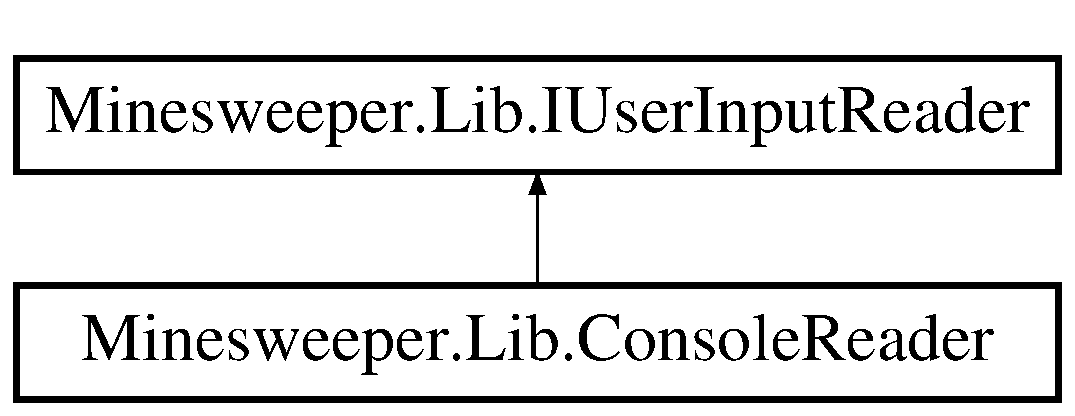
\includegraphics[height=2.000000cm]{interface_minesweeper_1_1_lib_1_1_i_user_input_reader}
\end{center}
\end{figure}
\subsection*{Public Member Functions}
\begin{DoxyCompactItemize}
\item 
string \hyperlink{interface_minesweeper_1_1_lib_1_1_i_user_input_reader_a58da9817d2e63a510cf833ce7d65f008}{Read\+Line} ()
\begin{DoxyCompactList}\small\item\em Reads the next line of characters from the input stream. \end{DoxyCompactList}\item 
void \hyperlink{interface_minesweeper_1_1_lib_1_1_i_user_input_reader_a54b4a65a7cea8be31dc99a6330be6f51}{Wait\+For\+Key} ()
\begin{DoxyCompactList}\small\item\em Waits for the user to press a key. \end{DoxyCompactList}\end{DoxyCompactItemize}


\subsection{Detailed Description}
Defines methods for reading user input. 



\subsection{Member Function Documentation}
\hypertarget{interface_minesweeper_1_1_lib_1_1_i_user_input_reader_a58da9817d2e63a510cf833ce7d65f008}{\index{Minesweeper\+::\+Lib\+::\+I\+User\+Input\+Reader@{Minesweeper\+::\+Lib\+::\+I\+User\+Input\+Reader}!Read\+Line@{Read\+Line}}
\index{Read\+Line@{Read\+Line}!Minesweeper\+::\+Lib\+::\+I\+User\+Input\+Reader@{Minesweeper\+::\+Lib\+::\+I\+User\+Input\+Reader}}
\subsubsection[{Read\+Line}]{\setlength{\rightskip}{0pt plus 5cm}string Minesweeper.\+Lib.\+I\+User\+Input\+Reader.\+Read\+Line (
\begin{DoxyParamCaption}
{}
\end{DoxyParamCaption}
)}}\label{interface_minesweeper_1_1_lib_1_1_i_user_input_reader_a58da9817d2e63a510cf833ce7d65f008}


Reads the next line of characters from the input stream. 

\begin{DoxyReturn}{Returns}
The next line of characters from the input stream, or null if no more lines are available.
\end{DoxyReturn}


Implemented in \hyperlink{class_minesweeper_1_1_lib_1_1_console_reader_ae6bb2ed667d1290078a0f9bb7b53e9a8}{Minesweeper.\+Lib.\+Console\+Reader}.

\hypertarget{interface_minesweeper_1_1_lib_1_1_i_user_input_reader_a54b4a65a7cea8be31dc99a6330be6f51}{\index{Minesweeper\+::\+Lib\+::\+I\+User\+Input\+Reader@{Minesweeper\+::\+Lib\+::\+I\+User\+Input\+Reader}!Wait\+For\+Key@{Wait\+For\+Key}}
\index{Wait\+For\+Key@{Wait\+For\+Key}!Minesweeper\+::\+Lib\+::\+I\+User\+Input\+Reader@{Minesweeper\+::\+Lib\+::\+I\+User\+Input\+Reader}}
\subsubsection[{Wait\+For\+Key}]{\setlength{\rightskip}{0pt plus 5cm}void Minesweeper.\+Lib.\+I\+User\+Input\+Reader.\+Wait\+For\+Key (
\begin{DoxyParamCaption}
{}
\end{DoxyParamCaption}
)}}\label{interface_minesweeper_1_1_lib_1_1_i_user_input_reader_a54b4a65a7cea8be31dc99a6330be6f51}


Waits for the user to press a key. 



Implemented in \hyperlink{class_minesweeper_1_1_lib_1_1_console_reader_a92588508515c5082d628e9f56672e863}{Minesweeper.\+Lib.\+Console\+Reader}.



The documentation for this interface was generated from the following file\+:\begin{DoxyCompactItemize}
\item 
Minesweeper/\+Minesweeper/\+Minesweeper.\+Lib/\+Interfaces/I\+User\+Input\+Reader.\+cs\end{DoxyCompactItemize}

\hypertarget{class_minesweeper_1_1_game_1_1_minefield}{\section{Minesweeper.\+Game.\+Minefield Class Reference}
\label{class_minesweeper_1_1_game_1_1_minefield}\index{Minesweeper.\+Game.\+Minefield@{Minesweeper.\+Game.\+Minefield}}
}


\hyperlink{class_minesweeper_1_1_game_1_1_minefield}{Minefield} class represents matrix of I\+Cell.  


Inheritance diagram for Minesweeper.\+Game.\+Minefield\+:\begin{figure}[H]
\begin{center}
\leavevmode
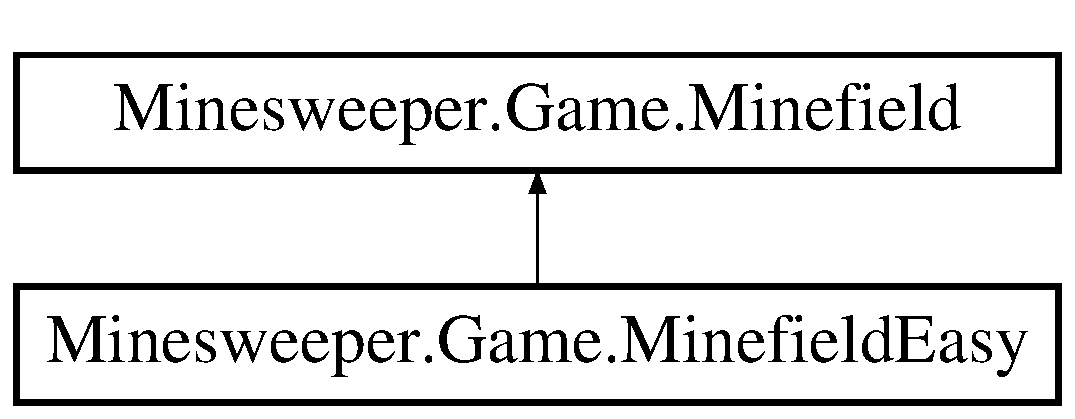
\includegraphics[height=2.000000cm]{class_minesweeper_1_1_game_1_1_minefield}
\end{center}
\end{figure}
\subsection*{Public Member Functions}
\begin{DoxyCompactItemize}
\item 
\hyperlink{class_minesweeper_1_1_game_1_1_minefield_ae13f75c03811d1808701a96b0daac034}{Minefield} (int rows, int cols, int number\+Of\+Mines, \hyperlink{interface_minesweeper_1_1_lib_1_1_i_random_generator_provider}{I\+Random\+Generator\+Provider} rnd\+Generator)
\begin{DoxyCompactList}\small\item\em Initializes a new instance of the \hyperlink{class_minesweeper_1_1_game_1_1_minefield}{Minefield} class. \end{DoxyCompactList}\item 
\hyperlink{namespace_minesweeper_af85e37deff295959aea34f4226d8ba93}{Cell\+Action\+Result} \hyperlink{class_minesweeper_1_1_game_1_1_minefield_a4238ded437c9cdf9fdfa5efb9be0e48f}{Open\+Cell\+Handler} (\hyperlink{interface_minesweeper_1_1_lib_1_1_i_cell_position}{I\+Cell\+Position} cell\+Position)
\begin{DoxyCompactList}\small\item\em Handles cell opening. Reveals cell's content and returns it's state. \end{DoxyCompactList}\item 
\hyperlink{namespace_minesweeper_af85e37deff295959aea34f4226d8ba93}{Cell\+Action\+Result} \hyperlink{class_minesweeper_1_1_game_1_1_minefield_a78fbb274c5004164c1eaf03564d5a8aa}{Flag\+Cell\+Handler} (\hyperlink{interface_minesweeper_1_1_lib_1_1_i_cell_position}{I\+Cell\+Position} cell\+Position)
\begin{DoxyCompactList}\small\item\em Handles cell flagging. \end{DoxyCompactList}\item 
\hyperlink{namespace_minesweeper_adf92d608047dafd69d16008492d317bd}{Cell\+Image}\mbox{[},\mbox{]} \hyperlink{class_minesweeper_1_1_game_1_1_minefield_a8bcfdd40f65d4c1c5e00565c880c8aa9}{Get\+Image} (bool show\+All=false)
\begin{DoxyCompactList}\small\item\em Gets an 'image' of the minefield as a matrix of type Cell\+Image. \end{DoxyCompactList}\item 
bool \hyperlink{class_minesweeper_1_1_game_1_1_minefield_a41bbc89242ced88cca3171e0c57fb50e}{Is\+Disarmed} ()
\begin{DoxyCompactList}\small\item\em Checks if all cells are opened without explosion. \end{DoxyCompactList}\end{DoxyCompactItemize}
\subsection*{Protected Member Functions}
\begin{DoxyCompactItemize}
\item 
bool \hyperlink{class_minesweeper_1_1_game_1_1_minefield_a1675fa664921d1110b8e2443645ce737}{Is\+Inside\+Matrix} (int row, int col)
\begin{DoxyCompactList}\small\item\em Validates if given coordinates are inside the minefield matrix. \end{DoxyCompactList}\item 
int \hyperlink{class_minesweeper_1_1_game_1_1_minefield_a18c96bbc37166965dcb92284f86cac0f}{Get\+Index} (\hyperlink{interface_minesweeper_1_1_lib_1_1_i_cell_position}{I\+Cell\+Position} cell)
\begin{DoxyCompactList}\small\item\em Converts (row,col) coordinates to index in the cell list. \end{DoxyCompactList}\item 
virtual bool \hyperlink{class_minesweeper_1_1_game_1_1_minefield_a5498de495abe8a57bc25e8a12babb08c}{Open\+Cell} (\hyperlink{interface_minesweeper_1_1_lib_1_1_i_cell_position}{I\+Cell\+Position} cell\+Position)
\begin{DoxyCompactList}\small\item\em Handles cell opening. Reveals cell's content and returns it's state. \end{DoxyCompactList}\end{DoxyCompactItemize}
\subsection*{Properties}
\begin{DoxyCompactItemize}
\item 
int\mbox{[},\mbox{]} \hyperlink{class_minesweeper_1_1_game_1_1_minefield_a6b62b86faae0edee06d71b14790661f1}{All\+Neighbor\+Mines}\hspace{0.3cm}{\ttfamily  \mbox{[}get\mbox{]}}
\begin{DoxyCompactList}\small\item\em Gets the number of neighbor mines for each cell. Returns copy of the all\+Neighbor\+Mines matrix. \end{DoxyCompactList}\item 
int \hyperlink{class_minesweeper_1_1_game_1_1_minefield_a3fabf570d9045ea288bb06fd1ecea287}{Opened\+Cells\+Count}\hspace{0.3cm}{\ttfamily  \mbox{[}get, set\mbox{]}}
\begin{DoxyCompactList}\small\item\em Gets or sets the number of opened cells in the minefield. \end{DoxyCompactList}\item 
I\+List$<$ \hyperlink{interface_minesweeper_1_1_lib_1_1_i_cell}{I\+Cell} $>$ \hyperlink{class_minesweeper_1_1_game_1_1_minefield_a6308163a3dc8ed1f5681de4bbd184788}{Cells}\hspace{0.3cm}{\ttfamily  \mbox{[}get, set\mbox{]}}
\begin{DoxyCompactList}\small\item\em Gets a list of cells in the minefield. \end{DoxyCompactList}\end{DoxyCompactItemize}


\subsection{Detailed Description}
\hyperlink{class_minesweeper_1_1_game_1_1_minefield}{Minefield} class represents matrix of I\+Cell. 



\subsection{Constructor \& Destructor Documentation}
\hypertarget{class_minesweeper_1_1_game_1_1_minefield_ae13f75c03811d1808701a96b0daac034}{\index{Minesweeper\+::\+Game\+::\+Minefield@{Minesweeper\+::\+Game\+::\+Minefield}!Minefield@{Minefield}}
\index{Minefield@{Minefield}!Minesweeper\+::\+Game\+::\+Minefield@{Minesweeper\+::\+Game\+::\+Minefield}}
\subsubsection[{Minefield}]{\setlength{\rightskip}{0pt plus 5cm}Minesweeper.\+Game.\+Minefield.\+Minefield (
\begin{DoxyParamCaption}
\item[{int}]{rows, }
\item[{int}]{cols, }
\item[{int}]{number\+Of\+Mines, }
\item[{{\bf I\+Random\+Generator\+Provider}}]{rnd\+Generator}
\end{DoxyParamCaption}
)}}\label{class_minesweeper_1_1_game_1_1_minefield_ae13f75c03811d1808701a96b0daac034}


Initializes a new instance of the \hyperlink{class_minesweeper_1_1_game_1_1_minefield}{Minefield} class. 


\begin{DoxyParams}{Parameters}
{\em rows} & Number of rows.\\
\hline
{\em cols} & Number of columns.\\
\hline
{\em number\+Of\+Mines} & Number of mines.\\
\hline
{\em rnd\+Generator} & Random generator provider.\\
\hline
\end{DoxyParams}


\subsection{Member Function Documentation}
\hypertarget{class_minesweeper_1_1_game_1_1_minefield_a78fbb274c5004164c1eaf03564d5a8aa}{\index{Minesweeper\+::\+Game\+::\+Minefield@{Minesweeper\+::\+Game\+::\+Minefield}!Flag\+Cell\+Handler@{Flag\+Cell\+Handler}}
\index{Flag\+Cell\+Handler@{Flag\+Cell\+Handler}!Minesweeper\+::\+Game\+::\+Minefield@{Minesweeper\+::\+Game\+::\+Minefield}}
\subsubsection[{Flag\+Cell\+Handler}]{\setlength{\rightskip}{0pt plus 5cm}{\bf Cell\+Action\+Result} Minesweeper.\+Game.\+Minefield.\+Flag\+Cell\+Handler (
\begin{DoxyParamCaption}
\item[{{\bf I\+Cell\+Position}}]{cell\+Position}
\end{DoxyParamCaption}
)}}\label{class_minesweeper_1_1_game_1_1_minefield_a78fbb274c5004164c1eaf03564d5a8aa}


Handles cell flagging. 


\begin{DoxyParams}{Parameters}
{\em cell\+Position} & Cell's position in the minefield matrix.\\
\hline
\end{DoxyParams}
\begin{DoxyReturn}{Returns}
State of the minefield.
\end{DoxyReturn}
\hypertarget{class_minesweeper_1_1_game_1_1_minefield_a8bcfdd40f65d4c1c5e00565c880c8aa9}{\index{Minesweeper\+::\+Game\+::\+Minefield@{Minesweeper\+::\+Game\+::\+Minefield}!Get\+Image@{Get\+Image}}
\index{Get\+Image@{Get\+Image}!Minesweeper\+::\+Game\+::\+Minefield@{Minesweeper\+::\+Game\+::\+Minefield}}
\subsubsection[{Get\+Image}]{\setlength{\rightskip}{0pt plus 5cm}{\bf Cell\+Image} \mbox{[},\mbox{]} Minesweeper.\+Game.\+Minefield.\+Get\+Image (
\begin{DoxyParamCaption}
\item[{bool}]{show\+All = {\ttfamily false}}
\end{DoxyParamCaption}
)}}\label{class_minesweeper_1_1_game_1_1_minefield_a8bcfdd40f65d4c1c5e00565c880c8aa9}


Gets an 'image' of the minefield as a matrix of type Cell\+Image. 


\begin{DoxyParams}{Parameters}
{\em show\+All} & Set to 'true' to uncover all mines.\\
\hline
\end{DoxyParams}
\begin{DoxyReturn}{Returns}
A matrix of cells of type Cell\+Image.
\end{DoxyReturn}
\hypertarget{class_minesweeper_1_1_game_1_1_minefield_a18c96bbc37166965dcb92284f86cac0f}{\index{Minesweeper\+::\+Game\+::\+Minefield@{Minesweeper\+::\+Game\+::\+Minefield}!Get\+Index@{Get\+Index}}
\index{Get\+Index@{Get\+Index}!Minesweeper\+::\+Game\+::\+Minefield@{Minesweeper\+::\+Game\+::\+Minefield}}
\subsubsection[{Get\+Index}]{\setlength{\rightskip}{0pt plus 5cm}int Minesweeper.\+Game.\+Minefield.\+Get\+Index (
\begin{DoxyParamCaption}
\item[{{\bf I\+Cell\+Position}}]{cell}
\end{DoxyParamCaption}
)\hspace{0.3cm}{\ttfamily [protected]}}}\label{class_minesweeper_1_1_game_1_1_minefield_a18c96bbc37166965dcb92284f86cac0f}


Converts (row,col) coordinates to index in the cell list. 


\begin{DoxyParams}{Parameters}
{\em cell} & The cell position.\\
\hline
\end{DoxyParams}
\begin{DoxyReturn}{Returns}
The index in the cell list.
\end{DoxyReturn}
\hypertarget{class_minesweeper_1_1_game_1_1_minefield_a41bbc89242ced88cca3171e0c57fb50e}{\index{Minesweeper\+::\+Game\+::\+Minefield@{Minesweeper\+::\+Game\+::\+Minefield}!Is\+Disarmed@{Is\+Disarmed}}
\index{Is\+Disarmed@{Is\+Disarmed}!Minesweeper\+::\+Game\+::\+Minefield@{Minesweeper\+::\+Game\+::\+Minefield}}
\subsubsection[{Is\+Disarmed}]{\setlength{\rightskip}{0pt plus 5cm}bool Minesweeper.\+Game.\+Minefield.\+Is\+Disarmed (
\begin{DoxyParamCaption}
{}
\end{DoxyParamCaption}
)}}\label{class_minesweeper_1_1_game_1_1_minefield_a41bbc89242ced88cca3171e0c57fb50e}


Checks if all cells are opened without explosion. 

\begin{DoxyReturn}{Returns}
True if all non-\/mined cells are opened.
\end{DoxyReturn}
\hypertarget{class_minesweeper_1_1_game_1_1_minefield_a1675fa664921d1110b8e2443645ce737}{\index{Minesweeper\+::\+Game\+::\+Minefield@{Minesweeper\+::\+Game\+::\+Minefield}!Is\+Inside\+Matrix@{Is\+Inside\+Matrix}}
\index{Is\+Inside\+Matrix@{Is\+Inside\+Matrix}!Minesweeper\+::\+Game\+::\+Minefield@{Minesweeper\+::\+Game\+::\+Minefield}}
\subsubsection[{Is\+Inside\+Matrix}]{\setlength{\rightskip}{0pt plus 5cm}bool Minesweeper.\+Game.\+Minefield.\+Is\+Inside\+Matrix (
\begin{DoxyParamCaption}
\item[{int}]{row, }
\item[{int}]{col}
\end{DoxyParamCaption}
)\hspace{0.3cm}{\ttfamily [protected]}}}\label{class_minesweeper_1_1_game_1_1_minefield_a1675fa664921d1110b8e2443645ce737}


Validates if given coordinates are inside the minefield matrix. 


\begin{DoxyParams}{Parameters}
{\em row} & Current position by row.\\
\hline
{\em col} & Current position by column.\\
\hline
\end{DoxyParams}
\begin{DoxyReturn}{Returns}
Validation result.
\end{DoxyReturn}
\hypertarget{class_minesweeper_1_1_game_1_1_minefield_a5498de495abe8a57bc25e8a12babb08c}{\index{Minesweeper\+::\+Game\+::\+Minefield@{Minesweeper\+::\+Game\+::\+Minefield}!Open\+Cell@{Open\+Cell}}
\index{Open\+Cell@{Open\+Cell}!Minesweeper\+::\+Game\+::\+Minefield@{Minesweeper\+::\+Game\+::\+Minefield}}
\subsubsection[{Open\+Cell}]{\setlength{\rightskip}{0pt plus 5cm}virtual bool Minesweeper.\+Game.\+Minefield.\+Open\+Cell (
\begin{DoxyParamCaption}
\item[{{\bf I\+Cell\+Position}}]{cell\+Position}
\end{DoxyParamCaption}
)\hspace{0.3cm}{\ttfamily [protected]}, {\ttfamily [virtual]}}}\label{class_minesweeper_1_1_game_1_1_minefield_a5498de495abe8a57bc25e8a12babb08c}


Handles cell opening. Reveals cell's content and returns it's state. 


\begin{DoxyParams}{Parameters}
{\em cell\+Position} & Cell's position in the minefield matrix.\\
\hline
\end{DoxyParams}
\begin{DoxyReturn}{Returns}
State of the minefield.
\end{DoxyReturn}


Reimplemented in \hyperlink{class_minesweeper_1_1_game_1_1_minefield_easy_ad66c9eb0e3876d537f2ea7a9f548410c}{Minesweeper.\+Game.\+Minefield\+Easy}.

\hypertarget{class_minesweeper_1_1_game_1_1_minefield_a4238ded437c9cdf9fdfa5efb9be0e48f}{\index{Minesweeper\+::\+Game\+::\+Minefield@{Minesweeper\+::\+Game\+::\+Minefield}!Open\+Cell\+Handler@{Open\+Cell\+Handler}}
\index{Open\+Cell\+Handler@{Open\+Cell\+Handler}!Minesweeper\+::\+Game\+::\+Minefield@{Minesweeper\+::\+Game\+::\+Minefield}}
\subsubsection[{Open\+Cell\+Handler}]{\setlength{\rightskip}{0pt plus 5cm}{\bf Cell\+Action\+Result} Minesweeper.\+Game.\+Minefield.\+Open\+Cell\+Handler (
\begin{DoxyParamCaption}
\item[{{\bf I\+Cell\+Position}}]{cell\+Position}
\end{DoxyParamCaption}
)}}\label{class_minesweeper_1_1_game_1_1_minefield_a4238ded437c9cdf9fdfa5efb9be0e48f}


Handles cell opening. Reveals cell's content and returns it's state. 


\begin{DoxyParams}{Parameters}
{\em cell\+Position} & Cell's position in the minefield matrix.\\
\hline
\end{DoxyParams}
\begin{DoxyReturn}{Returns}
State of the minefield.
\end{DoxyReturn}


\subsection{Property Documentation}
\hypertarget{class_minesweeper_1_1_game_1_1_minefield_a6b62b86faae0edee06d71b14790661f1}{\index{Minesweeper\+::\+Game\+::\+Minefield@{Minesweeper\+::\+Game\+::\+Minefield}!All\+Neighbor\+Mines@{All\+Neighbor\+Mines}}
\index{All\+Neighbor\+Mines@{All\+Neighbor\+Mines}!Minesweeper\+::\+Game\+::\+Minefield@{Minesweeper\+::\+Game\+::\+Minefield}}
\subsubsection[{All\+Neighbor\+Mines}]{\setlength{\rightskip}{0pt plus 5cm}int \mbox{[},\mbox{]} Minesweeper.\+Game.\+Minefield.\+All\+Neighbor\+Mines\hspace{0.3cm}{\ttfamily [get]}}}\label{class_minesweeper_1_1_game_1_1_minefield_a6b62b86faae0edee06d71b14790661f1}


Gets the number of neighbor mines for each cell. Returns copy of the all\+Neighbor\+Mines matrix. 

Not accepted.\hypertarget{class_minesweeper_1_1_game_1_1_minefield_a6308163a3dc8ed1f5681de4bbd184788}{\index{Minesweeper\+::\+Game\+::\+Minefield@{Minesweeper\+::\+Game\+::\+Minefield}!Cells@{Cells}}
\index{Cells@{Cells}!Minesweeper\+::\+Game\+::\+Minefield@{Minesweeper\+::\+Game\+::\+Minefield}}
\subsubsection[{Cells}]{\setlength{\rightskip}{0pt plus 5cm}I\+List$<${\bf I\+Cell}$>$ Minesweeper.\+Game.\+Minefield.\+Cells\hspace{0.3cm}{\ttfamily [get]}, {\ttfamily [set]}, {\ttfamily [protected]}}}\label{class_minesweeper_1_1_game_1_1_minefield_a6308163a3dc8ed1f5681de4bbd184788}


Gets a list of cells in the minefield. 

Not accepted.\hypertarget{class_minesweeper_1_1_game_1_1_minefield_a3fabf570d9045ea288bb06fd1ecea287}{\index{Minesweeper\+::\+Game\+::\+Minefield@{Minesweeper\+::\+Game\+::\+Minefield}!Opened\+Cells\+Count@{Opened\+Cells\+Count}}
\index{Opened\+Cells\+Count@{Opened\+Cells\+Count}!Minesweeper\+::\+Game\+::\+Minefield@{Minesweeper\+::\+Game\+::\+Minefield}}
\subsubsection[{Opened\+Cells\+Count}]{\setlength{\rightskip}{0pt plus 5cm}int Minesweeper.\+Game.\+Minefield.\+Opened\+Cells\+Count\hspace{0.3cm}{\ttfamily [get]}, {\ttfamily [set]}}}\label{class_minesweeper_1_1_game_1_1_minefield_a3fabf570d9045ea288bb06fd1ecea287}


Gets or sets the number of opened cells in the minefield. 

The number of opened cells.

The documentation for this class was generated from the following file\+:\begin{DoxyCompactItemize}
\item 
Minesweeper/\+Minesweeper/\+Minesweeper.\+game/Minefield.\+cs\end{DoxyCompactItemize}

\hypertarget{class_minesweeper_1_1_unit_tests_1_1_game_1_1_minefield_class_tests}{\section{Minesweeper.\+Unit\+Tests.\+Game.\+Minefield\+Class\+Tests Class Reference}
\label{class_minesweeper_1_1_unit_tests_1_1_game_1_1_minefield_class_tests}\index{Minesweeper.\+Unit\+Tests.\+Game.\+Minefield\+Class\+Tests@{Minesweeper.\+Unit\+Tests.\+Game.\+Minefield\+Class\+Tests}}
}
\subsection*{Public Member Functions}
\begin{DoxyCompactItemize}
\item 
\hypertarget{class_minesweeper_1_1_unit_tests_1_1_game_1_1_minefield_class_tests_a052364795ce9d9654108dafa6000f8b9}{void {\bfseries Initialize} ()}\label{class_minesweeper_1_1_unit_tests_1_1_game_1_1_minefield_class_tests_a052364795ce9d9654108dafa6000f8b9}

\item 
\hypertarget{class_minesweeper_1_1_unit_tests_1_1_game_1_1_minefield_class_tests_a85afc5fac3afefecd08fc1af0a3e3ac7}{void {\bfseries Minefield\+Constructor\+Recieving\+Null\+Random\+Generator\+Provider\+Should\+Throw\+An\+Exception} ()}\label{class_minesweeper_1_1_unit_tests_1_1_game_1_1_minefield_class_tests_a85afc5fac3afefecd08fc1af0a3e3ac7}

\item 
\hypertarget{class_minesweeper_1_1_unit_tests_1_1_game_1_1_minefield_class_tests_af73a594d83efcadb361e48fdb7254415}{void {\bfseries Minefield\+Constructor\+Recieving\+Incorrect\+Row\+Number\+Should\+Throw\+An\+Exception} ()}\label{class_minesweeper_1_1_unit_tests_1_1_game_1_1_minefield_class_tests_af73a594d83efcadb361e48fdb7254415}

\item 
\hypertarget{class_minesweeper_1_1_unit_tests_1_1_game_1_1_minefield_class_tests_a1e5e4ae4759228570a0af96fb1d1845f}{void {\bfseries Minefield\+Constructor\+Recieving\+Incorrect\+Column\+Number\+Should\+Throw\+An\+Exception} ()}\label{class_minesweeper_1_1_unit_tests_1_1_game_1_1_minefield_class_tests_a1e5e4ae4759228570a0af96fb1d1845f}

\item 
\hypertarget{class_minesweeper_1_1_unit_tests_1_1_game_1_1_minefield_class_tests_a91a4494bbf4cf458e92ec87392029037}{void {\bfseries Minefield\+Constructor\+Recieving\+Incorrect\+Mines\+Number\+Should\+Throw\+An\+Exception} ()}\label{class_minesweeper_1_1_unit_tests_1_1_game_1_1_minefield_class_tests_a91a4494bbf4cf458e92ec87392029037}

\item 
\hypertarget{class_minesweeper_1_1_unit_tests_1_1_game_1_1_minefield_class_tests_a619d46f5e743894b8b2b651c361aafff}{void {\bfseries All\+Neighbor\+Mines\+Property\+Should\+Return\+Correct\+Two\+Dimensional\+Array} ()}\label{class_minesweeper_1_1_unit_tests_1_1_game_1_1_minefield_class_tests_a619d46f5e743894b8b2b651c361aafff}

\item 
\hypertarget{class_minesweeper_1_1_unit_tests_1_1_game_1_1_minefield_class_tests_a5cb5109809a2da50ad015a3c3a334a6e}{void {\bfseries Open\+Cell\+Handler\+Should\+Miss\+The\+First\+Mine} ()}\label{class_minesweeper_1_1_unit_tests_1_1_game_1_1_minefield_class_tests_a5cb5109809a2da50ad015a3c3a334a6e}

\item 
\hypertarget{class_minesweeper_1_1_unit_tests_1_1_game_1_1_minefield_class_tests_a77bc1e8de7adf8b8edaf949507ec0e4a}{void {\bfseries Open\+Cell\+Handler\+Should\+Return\+Correct\+State\+Enumeration\+Value\+Boom} ()}\label{class_minesweeper_1_1_unit_tests_1_1_game_1_1_minefield_class_tests_a77bc1e8de7adf8b8edaf949507ec0e4a}

\item 
\hypertarget{class_minesweeper_1_1_unit_tests_1_1_game_1_1_minefield_class_tests_a4cab3954d245012a721e2a3364a3f471}{void {\bfseries Open\+Cell\+Handler\+Should\+Return\+Correct\+State\+Enumeration\+Value\+Normal\+Without\+Chained\+Opening} ()}\label{class_minesweeper_1_1_unit_tests_1_1_game_1_1_minefield_class_tests_a4cab3954d245012a721e2a3364a3f471}

\item 
\hypertarget{class_minesweeper_1_1_unit_tests_1_1_game_1_1_minefield_class_tests_ac496494fbd371f400aa91a0c12753efe}{void {\bfseries Open\+Cell\+Handler\+Should\+Return\+Correct\+State\+Enumeration\+Value\+Normal} ()}\label{class_minesweeper_1_1_unit_tests_1_1_game_1_1_minefield_class_tests_ac496494fbd371f400aa91a0c12753efe}

\item 
\hypertarget{class_minesweeper_1_1_unit_tests_1_1_game_1_1_minefield_class_tests_a12ca2a92bc3e3f04cfc33fd6a2aa9a70}{void {\bfseries Open\+Cell\+Handler\+Should\+Return\+Correct\+State\+Enumeration\+Value\+Already\+Opened} ()}\label{class_minesweeper_1_1_unit_tests_1_1_game_1_1_minefield_class_tests_a12ca2a92bc3e3f04cfc33fd6a2aa9a70}

\item 
\hypertarget{class_minesweeper_1_1_unit_tests_1_1_game_1_1_minefield_class_tests_a0b40e8aa707d0260c24d07675ddaa427}{void {\bfseries Open\+Cell\+Handler\+Should\+Return\+Correct\+State\+Enumeration\+Value\+Out\+Of\+Range} ()}\label{class_minesweeper_1_1_unit_tests_1_1_game_1_1_minefield_class_tests_a0b40e8aa707d0260c24d07675ddaa427}

\item 
\hypertarget{class_minesweeper_1_1_unit_tests_1_1_game_1_1_minefield_class_tests_af51b1f30a903fde456a6b258aab96a47}{void {\bfseries Get\+Image\+Should\+Return\+Proper\+Two\+Dimensional\+Array\+Of\+Cell\+Image\+Enums\+False\+Show\+All} ()}\label{class_minesweeper_1_1_unit_tests_1_1_game_1_1_minefield_class_tests_af51b1f30a903fde456a6b258aab96a47}

\item 
\hypertarget{class_minesweeper_1_1_unit_tests_1_1_game_1_1_minefield_class_tests_a9c6d456987ba9a68d4795361b58c63c9}{void {\bfseries Get\+Image\+Should\+Return\+Proper\+Two\+Dimensional\+Array\+Of\+Cell\+Image\+Enums\+True\+Show\+All} ()}\label{class_minesweeper_1_1_unit_tests_1_1_game_1_1_minefield_class_tests_a9c6d456987ba9a68d4795361b58c63c9}

\end{DoxyCompactItemize}
\subsection*{Static Public Member Functions}
\begin{DoxyCompactItemize}
\item 
\hypertarget{class_minesweeper_1_1_unit_tests_1_1_game_1_1_minefield_class_tests_a24435265c7ba64ddab0fd90e3d3e3ec0}{static void {\bfseries Class\+Initialize} (Test\+Context context)}\label{class_minesweeper_1_1_unit_tests_1_1_game_1_1_minefield_class_tests_a24435265c7ba64ddab0fd90e3d3e3ec0}

\end{DoxyCompactItemize}


The documentation for this class was generated from the following file\+:\begin{DoxyCompactItemize}
\item 
Minesweeper/\+Minesweeper/\+Minesweeper.\+Unit\+Tests/\+Game/Minefield\+Class\+Tests.\+cs\end{DoxyCompactItemize}

\hypertarget{class_minesweeper_1_1_game_1_1_minefield_easy}{\section{Minesweeper.\+Game.\+Minefield\+Easy Class Reference}
\label{class_minesweeper_1_1_game_1_1_minefield_easy}\index{Minesweeper.\+Game.\+Minefield\+Easy@{Minesweeper.\+Game.\+Minefield\+Easy}}
}


\hyperlink{class_minesweeper_1_1_game_1_1_minefield}{Minefield} class represents matrix of I\+Cell.  


Inheritance diagram for Minesweeper.\+Game.\+Minefield\+Easy\+:\begin{figure}[H]
\begin{center}
\leavevmode
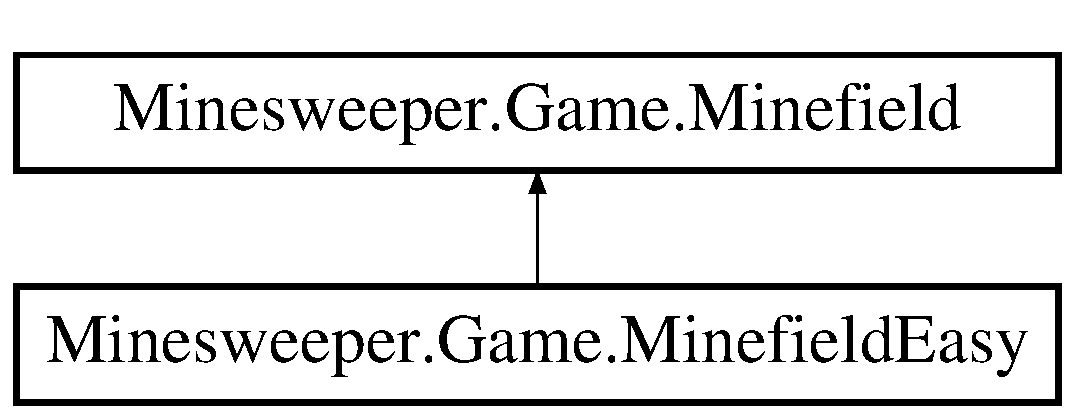
\includegraphics[height=2.000000cm]{class_minesweeper_1_1_game_1_1_minefield_easy}
\end{center}
\end{figure}
\subsection*{Public Member Functions}
\begin{DoxyCompactItemize}
\item 
\hyperlink{class_minesweeper_1_1_game_1_1_minefield_easy_acf546e6d351031a3e4840bcfd9a1cd77}{Minefield\+Easy} (int rows, int cols, int number\+Of\+Mines, \hyperlink{interface_minesweeper_1_1_lib_1_1_i_random_generator_provider}{I\+Random\+Generator\+Provider} rnd\+Generator)
\begin{DoxyCompactList}\small\item\em Initializes a new instance of the \hyperlink{class_minesweeper_1_1_game_1_1_minefield_easy}{Minefield\+Easy} class. \end{DoxyCompactList}\end{DoxyCompactItemize}
\subsection*{Protected Member Functions}
\begin{DoxyCompactItemize}
\item 
override bool \hyperlink{class_minesweeper_1_1_game_1_1_minefield_easy_ad66c9eb0e3876d537f2ea7a9f548410c}{Open\+Cell} (\hyperlink{interface_minesweeper_1_1_lib_1_1_i_cell_position}{I\+Cell\+Position} cell\+Position)
\begin{DoxyCompactList}\small\item\em Handles cell opening (recursively). Reveals cell's content and returns it's state. \end{DoxyCompactList}\end{DoxyCompactItemize}
\subsection*{Additional Inherited Members}


\subsection{Detailed Description}
\hyperlink{class_minesweeper_1_1_game_1_1_minefield}{Minefield} class represents matrix of I\+Cell. 



\subsection{Constructor \& Destructor Documentation}
\hypertarget{class_minesweeper_1_1_game_1_1_minefield_easy_acf546e6d351031a3e4840bcfd9a1cd77}{\index{Minesweeper\+::\+Game\+::\+Minefield\+Easy@{Minesweeper\+::\+Game\+::\+Minefield\+Easy}!Minefield\+Easy@{Minefield\+Easy}}
\index{Minefield\+Easy@{Minefield\+Easy}!Minesweeper\+::\+Game\+::\+Minefield\+Easy@{Minesweeper\+::\+Game\+::\+Minefield\+Easy}}
\subsubsection[{Minefield\+Easy}]{\setlength{\rightskip}{0pt plus 5cm}Minesweeper.\+Game.\+Minefield\+Easy.\+Minefield\+Easy (
\begin{DoxyParamCaption}
\item[{int}]{rows, }
\item[{int}]{cols, }
\item[{int}]{number\+Of\+Mines, }
\item[{{\bf I\+Random\+Generator\+Provider}}]{rnd\+Generator}
\end{DoxyParamCaption}
)}}\label{class_minesweeper_1_1_game_1_1_minefield_easy_acf546e6d351031a3e4840bcfd9a1cd77}


Initializes a new instance of the \hyperlink{class_minesweeper_1_1_game_1_1_minefield_easy}{Minefield\+Easy} class. 


\begin{DoxyParams}{Parameters}
{\em rows} & Number of rows.\\
\hline
{\em cols} & Number of columns.\\
\hline
{\em number\+Of\+Mines} & Number of mines.\\
\hline
{\em rnd\+Generator} & Random generator provider.\\
\hline
\end{DoxyParams}


\subsection{Member Function Documentation}
\hypertarget{class_minesweeper_1_1_game_1_1_minefield_easy_ad66c9eb0e3876d537f2ea7a9f548410c}{\index{Minesweeper\+::\+Game\+::\+Minefield\+Easy@{Minesweeper\+::\+Game\+::\+Minefield\+Easy}!Open\+Cell@{Open\+Cell}}
\index{Open\+Cell@{Open\+Cell}!Minesweeper\+::\+Game\+::\+Minefield\+Easy@{Minesweeper\+::\+Game\+::\+Minefield\+Easy}}
\subsubsection[{Open\+Cell}]{\setlength{\rightskip}{0pt plus 5cm}override bool Minesweeper.\+Game.\+Minefield\+Easy.\+Open\+Cell (
\begin{DoxyParamCaption}
\item[{{\bf I\+Cell\+Position}}]{cell\+Position}
\end{DoxyParamCaption}
)\hspace{0.3cm}{\ttfamily [protected]}, {\ttfamily [virtual]}}}\label{class_minesweeper_1_1_game_1_1_minefield_easy_ad66c9eb0e3876d537f2ea7a9f548410c}


Handles cell opening (recursively). Reveals cell's content and returns it's state. 


\begin{DoxyParams}{Parameters}
{\em cell\+Position} & Cell's position in the minefield matrix.\\
\hline
\end{DoxyParams}
\begin{DoxyReturn}{Returns}
State of the minefield.
\end{DoxyReturn}


Reimplemented from \hyperlink{class_minesweeper_1_1_game_1_1_minefield_a5498de495abe8a57bc25e8a12babb08c}{Minesweeper.\+Game.\+Minefield}.



The documentation for this class was generated from the following file\+:\begin{DoxyCompactItemize}
\item 
Minesweeper/\+Minesweeper/\+Minesweeper.\+game/Minefield\+Easy.\+cs\end{DoxyCompactItemize}

\hypertarget{class_minesweeper_1_1_unit_tests_1_1_game_1_1_minefield_easy_class_tests}{\section{Minesweeper.\+Unit\+Tests.\+Game.\+Minefield\+Easy\+Class\+Tests Class Reference}
\label{class_minesweeper_1_1_unit_tests_1_1_game_1_1_minefield_easy_class_tests}\index{Minesweeper.\+Unit\+Tests.\+Game.\+Minefield\+Easy\+Class\+Tests@{Minesweeper.\+Unit\+Tests.\+Game.\+Minefield\+Easy\+Class\+Tests}}
}
\subsection*{Public Member Functions}
\begin{DoxyCompactItemize}
\item 
\hypertarget{class_minesweeper_1_1_unit_tests_1_1_game_1_1_minefield_easy_class_tests_af1ac9c0942dae4d7d39985f3b276128d}{void {\bfseries Open\+Cell\+Handler\+Should\+Return\+Correct\+State\+Enumeration\+Value\+Normal\+Wth\+Chained\+Opening} ()}\label{class_minesweeper_1_1_unit_tests_1_1_game_1_1_minefield_easy_class_tests_af1ac9c0942dae4d7d39985f3b276128d}

\item 
\hypertarget{class_minesweeper_1_1_unit_tests_1_1_game_1_1_minefield_easy_class_tests_a09cdda447e48fa8542a0233c13ab5b7e}{void {\bfseries Open\+Cell\+Handler\+Should\+Open\+One\+Cell} ()}\label{class_minesweeper_1_1_unit_tests_1_1_game_1_1_minefield_easy_class_tests_a09cdda447e48fa8542a0233c13ab5b7e}

\end{DoxyCompactItemize}
\subsection*{Static Public Member Functions}
\begin{DoxyCompactItemize}
\item 
\hypertarget{class_minesweeper_1_1_unit_tests_1_1_game_1_1_minefield_easy_class_tests_a42609016f0a7b5c3efc3f5774d3cde2e}{static void {\bfseries Class\+Initialize} (Test\+Context context)}\label{class_minesweeper_1_1_unit_tests_1_1_game_1_1_minefield_easy_class_tests_a42609016f0a7b5c3efc3f5774d3cde2e}

\end{DoxyCompactItemize}


The documentation for this class was generated from the following file\+:\begin{DoxyCompactItemize}
\item 
Minesweeper/\+Minesweeper/\+Minesweeper.\+Unit\+Tests/\+Game/Minefield\+Easy\+Class\+Tests.\+cs\end{DoxyCompactItemize}

\hypertarget{class_minesweeper_1_1_game_1_1_minesweeper_game}{\section{Minesweeper.\+Game.\+Minesweeper\+Game Class Reference}
\label{class_minesweeper_1_1_game_1_1_minesweeper_game}\index{Minesweeper.\+Game.\+Minesweeper\+Game@{Minesweeper.\+Game.\+Minesweeper\+Game}}
}


The 'receiver' class in the Command pattern. Also a Facade for the \hyperlink{class_minesweeper_1_1_game_1_1_minefield}{Minefield}, \hyperlink{class_minesweeper_1_1_game_1_1_u_i_manager}{U\+I\+Manager} and \hyperlink{class_minesweeper_1_1_game_1_1_score_board}{Score\+Board} class. Uses Factory Method to create the minefield.  


Inheritance diagram for Minesweeper.\+Game.\+Minesweeper\+Game\+:\begin{figure}[H]
\begin{center}
\leavevmode
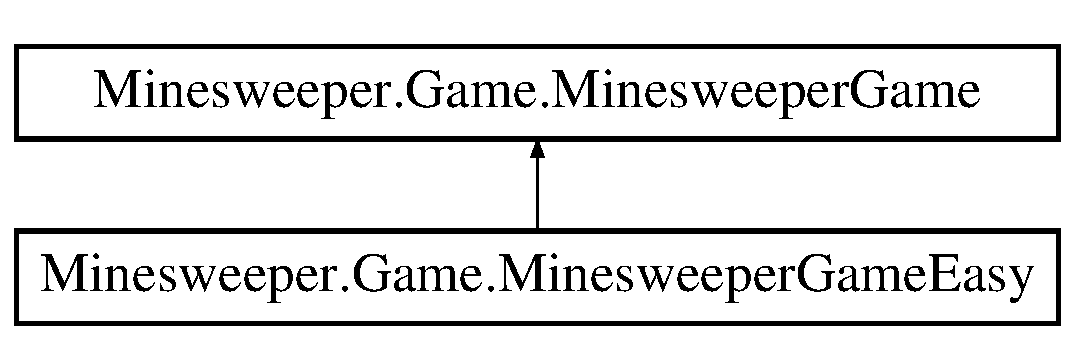
\includegraphics[height=2.000000cm]{class_minesweeper_1_1_game_1_1_minesweeper_game}
\end{center}
\end{figure}
\subsection*{Public Member Functions}
\begin{DoxyCompactItemize}
\item 
\hyperlink{class_minesweeper_1_1_game_1_1_minesweeper_game_a116b494ade82eea0125efb4541f22b23}{Minesweeper\+Game} (\hyperlink{interface_minesweeper_1_1_game_1_1_i_u_i_manager}{I\+U\+I\+Manager} ui\+Manager)
\begin{DoxyCompactList}\small\item\em Initializes a new instance of the \hyperlink{class_minesweeper_1_1_game_1_1_minesweeper_game}{Minesweeper.\+Game.\+Minesweeper\+Game} class. \end{DoxyCompactList}\item 
void \hyperlink{class_minesweeper_1_1_game_1_1_minesweeper_game_ab5b0c6535ef107b31e141fa6462f9b4c}{Open\+Cell} (\hyperlink{interface_minesweeper_1_1_lib_1_1_i_cell_position}{I\+Cell\+Position} cell)
\begin{DoxyCompactList}\small\item\em Opens the selected Cell \end{DoxyCompactList}\item 
void \hyperlink{class_minesweeper_1_1_game_1_1_minesweeper_game_a5c45da023c4d58c4c5cfc78336012b02}{Flag\+Cell} (\hyperlink{interface_minesweeper_1_1_lib_1_1_i_cell_position}{I\+Cell\+Position} cell)
\begin{DoxyCompactList}\small\item\em Flags the cell on the given coordinates. \end{DoxyCompactList}\item 
void \hyperlink{class_minesweeper_1_1_game_1_1_minesweeper_game_a53e6276fccb916310cece3d6ab9b3306}{Mine\+Boomed} ()
\begin{DoxyCompactList}\small\item\em When the mine explodes finishes the game and shows the appropriate message to the user. \end{DoxyCompactList}\item 
void \hyperlink{class_minesweeper_1_1_game_1_1_minesweeper_game_afb4bac8d31b4477b70e9618e9d28a621}{Exit\+Game} ()
\begin{DoxyCompactList}\small\item\em Method for quitting the game. \end{DoxyCompactList}\item 
void \hyperlink{class_minesweeper_1_1_game_1_1_minesweeper_game_a327c14748c81e511c4156c3e96290668}{Show\+Scores} ()
\begin{DoxyCompactList}\small\item\em Shows the high scores of the game. \end{DoxyCompactList}\item 
void \hyperlink{class_minesweeper_1_1_game_1_1_minesweeper_game_aa0a9944c0b3d78a2a322b1c8ecd2c19a}{Generate\+Minefield} ()
\begin{DoxyCompactList}\small\item\em Generates randomly mined minefield. \end{DoxyCompactList}\item 
void \hyperlink{class_minesweeper_1_1_game_1_1_minesweeper_game_aff1f0ecbb453fcdec86d441a3a56f834}{Display\+Error} ()
\begin{DoxyCompactList}\small\item\em Displays error message if the user enters invalid command. \end{DoxyCompactList}\end{DoxyCompactItemize}
\subsection*{Protected Member Functions}
\begin{DoxyCompactItemize}
\item 
abstract \hyperlink{class_minesweeper_1_1_game_1_1_minefield}{Minefield} \hyperlink{class_minesweeper_1_1_game_1_1_minesweeper_game_a44c9074e398f608490fa956a59c8e366}{Create\+Minefield} (int rows, int cols)
\begin{DoxyCompactList}\small\item\em Factory Method to create a new minefield. \end{DoxyCompactList}\end{DoxyCompactItemize}


\subsection{Detailed Description}
The 'receiver' class in the Command pattern. Also a Facade for the \hyperlink{class_minesweeper_1_1_game_1_1_minefield}{Minefield}, \hyperlink{class_minesweeper_1_1_game_1_1_u_i_manager}{U\+I\+Manager} and \hyperlink{class_minesweeper_1_1_game_1_1_score_board}{Score\+Board} class. Uses Factory Method to create the minefield. 



\subsection{Constructor \& Destructor Documentation}
\hypertarget{class_minesweeper_1_1_game_1_1_minesweeper_game_a116b494ade82eea0125efb4541f22b23}{\index{Minesweeper\+::\+Game\+::\+Minesweeper\+Game@{Minesweeper\+::\+Game\+::\+Minesweeper\+Game}!Minesweeper\+Game@{Minesweeper\+Game}}
\index{Minesweeper\+Game@{Minesweeper\+Game}!Minesweeper\+::\+Game\+::\+Minesweeper\+Game@{Minesweeper\+::\+Game\+::\+Minesweeper\+Game}}
\subsubsection[{Minesweeper\+Game}]{\setlength{\rightskip}{0pt plus 5cm}Minesweeper.\+Game.\+Minesweeper\+Game.\+Minesweeper\+Game (
\begin{DoxyParamCaption}
\item[{{\bf I\+U\+I\+Manager}}]{ui\+Manager}
\end{DoxyParamCaption}
)}}\label{class_minesweeper_1_1_game_1_1_minesweeper_game_a116b494ade82eea0125efb4541f22b23}


Initializes a new instance of the \hyperlink{class_minesweeper_1_1_game_1_1_minesweeper_game}{Minesweeper.\+Game.\+Minesweeper\+Game} class. 


\begin{DoxyParams}{Parameters}
{\em ui\+Manager} & The \hyperlink{interface_minesweeper_1_1_game_1_1_i_u_i_manager}{Minesweeper.\+Game.\+I\+U\+I\+Manager} implementation used to read and write.\\
\hline
\end{DoxyParams}


\subsection{Member Function Documentation}
\hypertarget{class_minesweeper_1_1_game_1_1_minesweeper_game_a44c9074e398f608490fa956a59c8e366}{\index{Minesweeper\+::\+Game\+::\+Minesweeper\+Game@{Minesweeper\+::\+Game\+::\+Minesweeper\+Game}!Create\+Minefield@{Create\+Minefield}}
\index{Create\+Minefield@{Create\+Minefield}!Minesweeper\+::\+Game\+::\+Minesweeper\+Game@{Minesweeper\+::\+Game\+::\+Minesweeper\+Game}}
\subsubsection[{Create\+Minefield}]{\setlength{\rightskip}{0pt plus 5cm}abstract {\bf Minefield} Minesweeper.\+Game.\+Minesweeper\+Game.\+Create\+Minefield (
\begin{DoxyParamCaption}
\item[{int}]{rows, }
\item[{int}]{cols}
\end{DoxyParamCaption}
)\hspace{0.3cm}{\ttfamily [protected]}, {\ttfamily [pure virtual]}}}\label{class_minesweeper_1_1_game_1_1_minesweeper_game_a44c9074e398f608490fa956a59c8e366}


Factory Method to create a new minefield. 


\begin{DoxyParams}{Parameters}
{\em rows} & Rows in the minefield.\\
\hline
{\em cols} & Columns in the minefield.\\
\hline
\end{DoxyParams}
\begin{DoxyReturn}{Returns}
Returns a new minefield.
\end{DoxyReturn}


Implemented in \hyperlink{class_minesweeper_1_1_game_1_1_minesweeper_game_easy_a9f01271eaaabb3d027d00b2677d6995c}{Minesweeper.\+Game.\+Minesweeper\+Game\+Easy}.

\hypertarget{class_minesweeper_1_1_game_1_1_minesweeper_game_aff1f0ecbb453fcdec86d441a3a56f834}{\index{Minesweeper\+::\+Game\+::\+Minesweeper\+Game@{Minesweeper\+::\+Game\+::\+Minesweeper\+Game}!Display\+Error@{Display\+Error}}
\index{Display\+Error@{Display\+Error}!Minesweeper\+::\+Game\+::\+Minesweeper\+Game@{Minesweeper\+::\+Game\+::\+Minesweeper\+Game}}
\subsubsection[{Display\+Error}]{\setlength{\rightskip}{0pt plus 5cm}void Minesweeper.\+Game.\+Minesweeper\+Game.\+Display\+Error (
\begin{DoxyParamCaption}
{}
\end{DoxyParamCaption}
)}}\label{class_minesweeper_1_1_game_1_1_minesweeper_game_aff1f0ecbb453fcdec86d441a3a56f834}


Displays error message if the user enters invalid command. 

\hypertarget{class_minesweeper_1_1_game_1_1_minesweeper_game_afb4bac8d31b4477b70e9618e9d28a621}{\index{Minesweeper\+::\+Game\+::\+Minesweeper\+Game@{Minesweeper\+::\+Game\+::\+Minesweeper\+Game}!Exit\+Game@{Exit\+Game}}
\index{Exit\+Game@{Exit\+Game}!Minesweeper\+::\+Game\+::\+Minesweeper\+Game@{Minesweeper\+::\+Game\+::\+Minesweeper\+Game}}
\subsubsection[{Exit\+Game}]{\setlength{\rightskip}{0pt plus 5cm}void Minesweeper.\+Game.\+Minesweeper\+Game.\+Exit\+Game (
\begin{DoxyParamCaption}
{}
\end{DoxyParamCaption}
)}}\label{class_minesweeper_1_1_game_1_1_minesweeper_game_afb4bac8d31b4477b70e9618e9d28a621}


Method for quitting the game. 

\hypertarget{class_minesweeper_1_1_game_1_1_minesweeper_game_a5c45da023c4d58c4c5cfc78336012b02}{\index{Minesweeper\+::\+Game\+::\+Minesweeper\+Game@{Minesweeper\+::\+Game\+::\+Minesweeper\+Game}!Flag\+Cell@{Flag\+Cell}}
\index{Flag\+Cell@{Flag\+Cell}!Minesweeper\+::\+Game\+::\+Minesweeper\+Game@{Minesweeper\+::\+Game\+::\+Minesweeper\+Game}}
\subsubsection[{Flag\+Cell}]{\setlength{\rightskip}{0pt plus 5cm}void Minesweeper.\+Game.\+Minesweeper\+Game.\+Flag\+Cell (
\begin{DoxyParamCaption}
\item[{{\bf I\+Cell\+Position}}]{cell}
\end{DoxyParamCaption}
)}}\label{class_minesweeper_1_1_game_1_1_minesweeper_game_a5c45da023c4d58c4c5cfc78336012b02}


Flags the cell on the given coordinates. 


\begin{DoxyParams}{Parameters}
{\em cell} & The position of the cell.\\
\hline
\end{DoxyParams}
\hypertarget{class_minesweeper_1_1_game_1_1_minesweeper_game_aa0a9944c0b3d78a2a322b1c8ecd2c19a}{\index{Minesweeper\+::\+Game\+::\+Minesweeper\+Game@{Minesweeper\+::\+Game\+::\+Minesweeper\+Game}!Generate\+Minefield@{Generate\+Minefield}}
\index{Generate\+Minefield@{Generate\+Minefield}!Minesweeper\+::\+Game\+::\+Minesweeper\+Game@{Minesweeper\+::\+Game\+::\+Minesweeper\+Game}}
\subsubsection[{Generate\+Minefield}]{\setlength{\rightskip}{0pt plus 5cm}void Minesweeper.\+Game.\+Minesweeper\+Game.\+Generate\+Minefield (
\begin{DoxyParamCaption}
{}
\end{DoxyParamCaption}
)}}\label{class_minesweeper_1_1_game_1_1_minesweeper_game_aa0a9944c0b3d78a2a322b1c8ecd2c19a}


Generates randomly mined minefield. 

\hypertarget{class_minesweeper_1_1_game_1_1_minesweeper_game_a53e6276fccb916310cece3d6ab9b3306}{\index{Minesweeper\+::\+Game\+::\+Minesweeper\+Game@{Minesweeper\+::\+Game\+::\+Minesweeper\+Game}!Mine\+Boomed@{Mine\+Boomed}}
\index{Mine\+Boomed@{Mine\+Boomed}!Minesweeper\+::\+Game\+::\+Minesweeper\+Game@{Minesweeper\+::\+Game\+::\+Minesweeper\+Game}}
\subsubsection[{Mine\+Boomed}]{\setlength{\rightskip}{0pt plus 5cm}void Minesweeper.\+Game.\+Minesweeper\+Game.\+Mine\+Boomed (
\begin{DoxyParamCaption}
{}
\end{DoxyParamCaption}
)}}\label{class_minesweeper_1_1_game_1_1_minesweeper_game_a53e6276fccb916310cece3d6ab9b3306}


When the mine explodes finishes the game and shows the appropriate message to the user. 

\hypertarget{class_minesweeper_1_1_game_1_1_minesweeper_game_ab5b0c6535ef107b31e141fa6462f9b4c}{\index{Minesweeper\+::\+Game\+::\+Minesweeper\+Game@{Minesweeper\+::\+Game\+::\+Minesweeper\+Game}!Open\+Cell@{Open\+Cell}}
\index{Open\+Cell@{Open\+Cell}!Minesweeper\+::\+Game\+::\+Minesweeper\+Game@{Minesweeper\+::\+Game\+::\+Minesweeper\+Game}}
\subsubsection[{Open\+Cell}]{\setlength{\rightskip}{0pt plus 5cm}void Minesweeper.\+Game.\+Minesweeper\+Game.\+Open\+Cell (
\begin{DoxyParamCaption}
\item[{{\bf I\+Cell\+Position}}]{cell}
\end{DoxyParamCaption}
)}}\label{class_minesweeper_1_1_game_1_1_minesweeper_game_ab5b0c6535ef107b31e141fa6462f9b4c}


Opens the selected Cell 


\begin{DoxyParams}{Parameters}
{\em cell} & The position of the cell on the minefield.\\
\hline
\end{DoxyParams}
\hypertarget{class_minesweeper_1_1_game_1_1_minesweeper_game_a327c14748c81e511c4156c3e96290668}{\index{Minesweeper\+::\+Game\+::\+Minesweeper\+Game@{Minesweeper\+::\+Game\+::\+Minesweeper\+Game}!Show\+Scores@{Show\+Scores}}
\index{Show\+Scores@{Show\+Scores}!Minesweeper\+::\+Game\+::\+Minesweeper\+Game@{Minesweeper\+::\+Game\+::\+Minesweeper\+Game}}
\subsubsection[{Show\+Scores}]{\setlength{\rightskip}{0pt plus 5cm}void Minesweeper.\+Game.\+Minesweeper\+Game.\+Show\+Scores (
\begin{DoxyParamCaption}
{}
\end{DoxyParamCaption}
)}}\label{class_minesweeper_1_1_game_1_1_minesweeper_game_a327c14748c81e511c4156c3e96290668}


Shows the high scores of the game. 



The documentation for this class was generated from the following file\+:\begin{DoxyCompactItemize}
\item 
Minesweeper/\+Minesweeper/\+Minesweeper.\+game/Minesweeper\+Game.\+cs\end{DoxyCompactItemize}

\hypertarget{class_minesweeper_1_1_game_1_1_minesweeper_game_easy}{\section{Minesweeper.\+Game.\+Minesweeper\+Game\+Easy Class Reference}
\label{class_minesweeper_1_1_game_1_1_minesweeper_game_easy}\index{Minesweeper.\+Game.\+Minesweeper\+Game\+Easy@{Minesweeper.\+Game.\+Minesweeper\+Game\+Easy}}
}


Overrides the factory method to return an instance of the \hyperlink{class_minesweeper_1_1_game_1_1_minefield}{Minefield} class.  


Inheritance diagram for Minesweeper.\+Game.\+Minesweeper\+Game\+Easy\+:\begin{figure}[H]
\begin{center}
\leavevmode
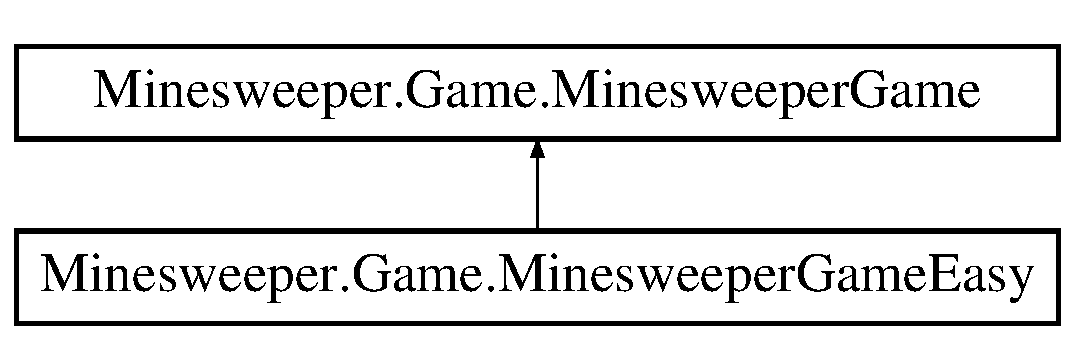
\includegraphics[height=2.000000cm]{class_minesweeper_1_1_game_1_1_minesweeper_game_easy}
\end{center}
\end{figure}
\subsection*{Public Member Functions}
\begin{DoxyCompactItemize}
\item 
\hyperlink{class_minesweeper_1_1_game_1_1_minesweeper_game_easy_a19034dce499f785fe6abc0684f47cc87}{Minesweeper\+Game\+Easy} (\hyperlink{interface_minesweeper_1_1_game_1_1_i_u_i_manager}{I\+U\+I\+Manager} ui\+Manager)
\begin{DoxyCompactList}\small\item\em Initializes a new instance of the \hyperlink{class_minesweeper_1_1_game_1_1_minesweeper_game_easy}{Minesweeper.\+Game.\+Minesweeper\+Game\+Easy} class. \end{DoxyCompactList}\end{DoxyCompactItemize}
\subsection*{Protected Member Functions}
\begin{DoxyCompactItemize}
\item 
override \hyperlink{class_minesweeper_1_1_game_1_1_minefield}{Minefield} \hyperlink{class_minesweeper_1_1_game_1_1_minesweeper_game_easy_a9f01271eaaabb3d027d00b2677d6995c}{Create\+Minefield} (int rows, int cols)
\begin{DoxyCompactList}\small\item\em Factory Method implementation to create a new minefield. \end{DoxyCompactList}\end{DoxyCompactItemize}


\subsection{Detailed Description}
Overrides the factory method to return an instance of the \hyperlink{class_minesweeper_1_1_game_1_1_minefield}{Minefield} class. 



\subsection{Constructor \& Destructor Documentation}
\hypertarget{class_minesweeper_1_1_game_1_1_minesweeper_game_easy_a19034dce499f785fe6abc0684f47cc87}{\index{Minesweeper\+::\+Game\+::\+Minesweeper\+Game\+Easy@{Minesweeper\+::\+Game\+::\+Minesweeper\+Game\+Easy}!Minesweeper\+Game\+Easy@{Minesweeper\+Game\+Easy}}
\index{Minesweeper\+Game\+Easy@{Minesweeper\+Game\+Easy}!Minesweeper\+::\+Game\+::\+Minesweeper\+Game\+Easy@{Minesweeper\+::\+Game\+::\+Minesweeper\+Game\+Easy}}
\subsubsection[{Minesweeper\+Game\+Easy}]{\setlength{\rightskip}{0pt plus 5cm}Minesweeper.\+Game.\+Minesweeper\+Game\+Easy.\+Minesweeper\+Game\+Easy (
\begin{DoxyParamCaption}
\item[{{\bf I\+U\+I\+Manager}}]{ui\+Manager}
\end{DoxyParamCaption}
)}}\label{class_minesweeper_1_1_game_1_1_minesweeper_game_easy_a19034dce499f785fe6abc0684f47cc87}


Initializes a new instance of the \hyperlink{class_minesweeper_1_1_game_1_1_minesweeper_game_easy}{Minesweeper.\+Game.\+Minesweeper\+Game\+Easy} class. 


\begin{DoxyParams}{Parameters}
{\em ui\+Manager} & The \hyperlink{interface_minesweeper_1_1_game_1_1_i_u_i_manager}{Minesweeper.\+Game.\+I\+U\+I\+Manager} implementation used to read and write.\\
\hline
\end{DoxyParams}


\subsection{Member Function Documentation}
\hypertarget{class_minesweeper_1_1_game_1_1_minesweeper_game_easy_a9f01271eaaabb3d027d00b2677d6995c}{\index{Minesweeper\+::\+Game\+::\+Minesweeper\+Game\+Easy@{Minesweeper\+::\+Game\+::\+Minesweeper\+Game\+Easy}!Create\+Minefield@{Create\+Minefield}}
\index{Create\+Minefield@{Create\+Minefield}!Minesweeper\+::\+Game\+::\+Minesweeper\+Game\+Easy@{Minesweeper\+::\+Game\+::\+Minesweeper\+Game\+Easy}}
\subsubsection[{Create\+Minefield}]{\setlength{\rightskip}{0pt plus 5cm}override {\bf Minefield} Minesweeper.\+Game.\+Minesweeper\+Game\+Easy.\+Create\+Minefield (
\begin{DoxyParamCaption}
\item[{int}]{rows, }
\item[{int}]{cols}
\end{DoxyParamCaption}
)\hspace{0.3cm}{\ttfamily [protected]}, {\ttfamily [virtual]}}}\label{class_minesweeper_1_1_game_1_1_minesweeper_game_easy_a9f01271eaaabb3d027d00b2677d6995c}


Factory Method implementation to create a new minefield. 


\begin{DoxyParams}{Parameters}
{\em rows} & Rows in the minefield.\\
\hline
{\em cols} & Columns in the minefield.\\
\hline
\end{DoxyParams}
\begin{DoxyReturn}{Returns}
Returns a new minefield.
\end{DoxyReturn}


Implements \hyperlink{class_minesweeper_1_1_game_1_1_minesweeper_game_a44c9074e398f608490fa956a59c8e366}{Minesweeper.\+Game.\+Minesweeper\+Game}.



The documentation for this class was generated from the following file\+:\begin{DoxyCompactItemize}
\item 
Minesweeper/\+Minesweeper/\+Minesweeper.\+game/Minesweeper\+Game\+Easy.\+cs\end{DoxyCompactItemize}

\hypertarget{class_minesweeper_1_1_game_1_1_program}{\section{Minesweeper.\+Game.\+Program Class Reference}
\label{class_minesweeper_1_1_game_1_1_program}\index{Minesweeper.\+Game.\+Program@{Minesweeper.\+Game.\+Program}}
}


Class for the main entry point of the program.  


\subsection*{Static Public Member Functions}
\begin{DoxyCompactItemize}
\item 
static void \hyperlink{class_minesweeper_1_1_game_1_1_program_aa3806b8f251144cbba0f7c44890e64ce}{Main} ()
\begin{DoxyCompactList}\small\item\em The entry point of the console application. \end{DoxyCompactList}\end{DoxyCompactItemize}


\subsection{Detailed Description}
Class for the main entry point of the program. 



\subsection{Member Function Documentation}
\hypertarget{class_minesweeper_1_1_game_1_1_program_aa3806b8f251144cbba0f7c44890e64ce}{\index{Minesweeper\+::\+Game\+::\+Program@{Minesweeper\+::\+Game\+::\+Program}!Main@{Main}}
\index{Main@{Main}!Minesweeper\+::\+Game\+::\+Program@{Minesweeper\+::\+Game\+::\+Program}}
\subsubsection[{Main}]{\setlength{\rightskip}{0pt plus 5cm}static void Minesweeper.\+Game.\+Program.\+Main (
\begin{DoxyParamCaption}
{}
\end{DoxyParamCaption}
)\hspace{0.3cm}{\ttfamily [static]}}}\label{class_minesweeper_1_1_game_1_1_program_aa3806b8f251144cbba0f7c44890e64ce}


The entry point of the console application. 



The documentation for this class was generated from the following file\+:\begin{DoxyCompactItemize}
\item 
Minesweeper/\+Minesweeper/\+Minesweeper.\+game/Program.\+cs\end{DoxyCompactItemize}

\hypertarget{class_minesweeper_1_1_lib_1_1_random_generator_provider}{\section{Minesweeper.\+Lib.\+Random\+Generator\+Provider Class Reference}
\label{class_minesweeper_1_1_lib_1_1_random_generator_provider}\index{Minesweeper.\+Lib.\+Random\+Generator\+Provider@{Minesweeper.\+Lib.\+Random\+Generator\+Provider}}
}


Random generator singleton.  


Inheritance diagram for Minesweeper.\+Lib.\+Random\+Generator\+Provider\+:\begin{figure}[H]
\begin{center}
\leavevmode
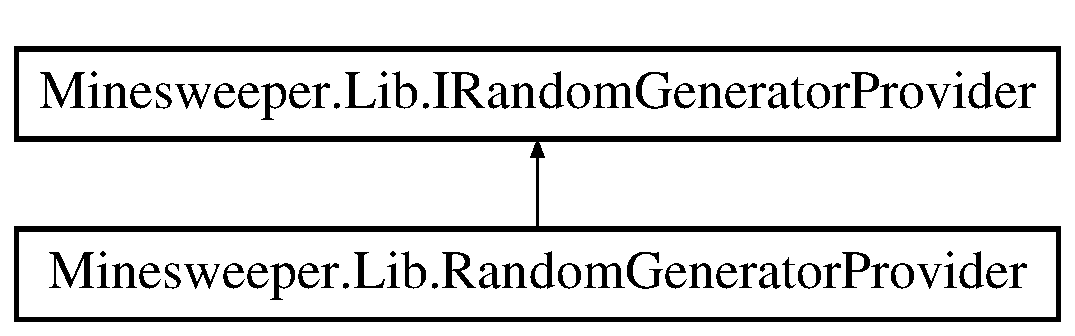
\includegraphics[height=2.000000cm]{class_minesweeper_1_1_lib_1_1_random_generator_provider}
\end{center}
\end{figure}
\subsection*{Public Member Functions}
\begin{DoxyCompactItemize}
\item 
int \hyperlink{class_minesweeper_1_1_lib_1_1_random_generator_provider_a53e1e507758a05548dd09e14c81af8d4}{Next} (int min\+Number, int max\+Number)
\begin{DoxyCompactList}\small\item\em Generates random number through Random class. \end{DoxyCompactList}\item 
int \hyperlink{class_minesweeper_1_1_lib_1_1_random_generator_provider_afabb9a038955a531abcb19cb0c6b77a3}{Next} (int max\+Number)
\begin{DoxyCompactList}\small\item\em Overload with minimal range 0. \end{DoxyCompactList}\end{DoxyCompactItemize}
\subsection*{Static Public Member Functions}
\begin{DoxyCompactItemize}
\item 
static \hyperlink{class_minesweeper_1_1_lib_1_1_random_generator_provider}{Random\+Generator\+Provider} \hyperlink{class_minesweeper_1_1_lib_1_1_random_generator_provider_ab8f03e8ad898e70caa96d13e80f750b4}{Get\+Instance} ()
\begin{DoxyCompactList}\small\item\em Returns the only instance of \hyperlink{class_minesweeper_1_1_lib_1_1_random_generator_provider}{Random\+Generator\+Provider}. \end{DoxyCompactList}\end{DoxyCompactItemize}


\subsection{Detailed Description}
Random generator singleton. 



\subsection{Member Function Documentation}
\hypertarget{class_minesweeper_1_1_lib_1_1_random_generator_provider_ab8f03e8ad898e70caa96d13e80f750b4}{\index{Minesweeper\+::\+Lib\+::\+Random\+Generator\+Provider@{Minesweeper\+::\+Lib\+::\+Random\+Generator\+Provider}!Get\+Instance@{Get\+Instance}}
\index{Get\+Instance@{Get\+Instance}!Minesweeper\+::\+Lib\+::\+Random\+Generator\+Provider@{Minesweeper\+::\+Lib\+::\+Random\+Generator\+Provider}}
\subsubsection[{Get\+Instance}]{\setlength{\rightskip}{0pt plus 5cm}static {\bf Random\+Generator\+Provider} Minesweeper.\+Lib.\+Random\+Generator\+Provider.\+Get\+Instance (
\begin{DoxyParamCaption}
{}
\end{DoxyParamCaption}
)\hspace{0.3cm}{\ttfamily [static]}}}\label{class_minesweeper_1_1_lib_1_1_random_generator_provider_ab8f03e8ad898e70caa96d13e80f750b4}


Returns the only instance of \hyperlink{class_minesweeper_1_1_lib_1_1_random_generator_provider}{Random\+Generator\+Provider}. 

\begin{DoxyReturn}{Returns}
\hyperlink{class_minesweeper_1_1_lib_1_1_random_generator_provider}{Random\+Generator\+Provider} only instance.
\end{DoxyReturn}
\hypertarget{class_minesweeper_1_1_lib_1_1_random_generator_provider_a53e1e507758a05548dd09e14c81af8d4}{\index{Minesweeper\+::\+Lib\+::\+Random\+Generator\+Provider@{Minesweeper\+::\+Lib\+::\+Random\+Generator\+Provider}!Next@{Next}}
\index{Next@{Next}!Minesweeper\+::\+Lib\+::\+Random\+Generator\+Provider@{Minesweeper\+::\+Lib\+::\+Random\+Generator\+Provider}}
\subsubsection[{Next}]{\setlength{\rightskip}{0pt plus 5cm}int Minesweeper.\+Lib.\+Random\+Generator\+Provider.\+Next (
\begin{DoxyParamCaption}
\item[{int}]{min\+Number, }
\item[{int}]{max\+Number}
\end{DoxyParamCaption}
)}}\label{class_minesweeper_1_1_lib_1_1_random_generator_provider_a53e1e507758a05548dd09e14c81af8d4}


Generates random number through Random class. 


\begin{DoxyParams}{Parameters}
{\em min\+Number} & Minimal range.\\
\hline
{\em max\+Number} & Maximal range.\\
\hline
\end{DoxyParams}
\begin{DoxyReturn}{Returns}
Integer random number.
\end{DoxyReturn}


Implements \hyperlink{interface_minesweeper_1_1_lib_1_1_i_random_generator_provider_a0f49fa42c327f257a83bfb9264cb9124}{Minesweeper.\+Lib.\+I\+Random\+Generator\+Provider}.

\hypertarget{class_minesweeper_1_1_lib_1_1_random_generator_provider_afabb9a038955a531abcb19cb0c6b77a3}{\index{Minesweeper\+::\+Lib\+::\+Random\+Generator\+Provider@{Minesweeper\+::\+Lib\+::\+Random\+Generator\+Provider}!Next@{Next}}
\index{Next@{Next}!Minesweeper\+::\+Lib\+::\+Random\+Generator\+Provider@{Minesweeper\+::\+Lib\+::\+Random\+Generator\+Provider}}
\subsubsection[{Next}]{\setlength{\rightskip}{0pt plus 5cm}int Minesweeper.\+Lib.\+Random\+Generator\+Provider.\+Next (
\begin{DoxyParamCaption}
\item[{int}]{max\+Number}
\end{DoxyParamCaption}
)}}\label{class_minesweeper_1_1_lib_1_1_random_generator_provider_afabb9a038955a531abcb19cb0c6b77a3}


Overload with minimal range 0. 


\begin{DoxyParams}{Parameters}
{\em max\+Number} & Maximal range.\\
\hline
\end{DoxyParams}
\begin{DoxyReturn}{Returns}
Integer random number.
\end{DoxyReturn}


Implements \hyperlink{interface_minesweeper_1_1_lib_1_1_i_random_generator_provider_a582bbebd6de2ecdded37c76b35c74a66}{Minesweeper.\+Lib.\+I\+Random\+Generator\+Provider}.



The documentation for this class was generated from the following file\+:\begin{DoxyCompactItemize}
\item 
Minesweeper/\+Minesweeper/\+Minesweeper.\+Lib/Random\+Generator\+Provider.\+cs\end{DoxyCompactItemize}

\hypertarget{class_minesweeper_1_1_game_1_1_score_board}{\section{Minesweeper.\+Game.\+Score\+Board Class Reference}
\label{class_minesweeper_1_1_game_1_1_score_board}\index{Minesweeper.\+Game.\+Score\+Board@{Minesweeper.\+Game.\+Score\+Board}}
}


\hyperlink{class_minesweeper_1_1_game_1_1_score_board}{Score\+Board} class that stores and updates the top scores for the game.  


\subsection*{Public Member Functions}
\begin{DoxyCompactItemize}
\item 
\hyperlink{class_minesweeper_1_1_game_1_1_score_board_a30a6adbef4b4a9c0c7720df2725d3bf5}{Score\+Board} ()
\begin{DoxyCompactList}\small\item\em Initializes a new instance of the \hyperlink{class_minesweeper_1_1_game_1_1_score_board}{Score\+Board} class. \end{DoxyCompactList}\item 
void \hyperlink{class_minesweeper_1_1_game_1_1_score_board_acb8f228b35af71c1bd91012e32be4283}{Add\+Score} (string name, int number\+Of\+Opened\+Cells)
\begin{DoxyCompactList}\small\item\em Adds the current player high score. Player will not be added if the score is lower than the lowest score. \end{DoxyCompactList}\end{DoxyCompactItemize}
\subsection*{Properties}
\begin{DoxyCompactItemize}
\item 
I\+Enumerable$<$ Key\+Value\+Pair\\*
$<$ string, int $>$ $>$ \hyperlink{class_minesweeper_1_1_game_1_1_score_board_a009d2aa35647d16eb0b6aa89943d01ac}{Top\+Scores}\hspace{0.3cm}{\ttfamily  \mbox{[}get\mbox{]}}
\begin{DoxyCompactList}\small\item\em Gets a sorted list of the top scores as \mbox{[}name, score\mbox{]} pairs. \end{DoxyCompactList}\end{DoxyCompactItemize}


\subsection{Detailed Description}
\hyperlink{class_minesweeper_1_1_game_1_1_score_board}{Score\+Board} class that stores and updates the top scores for the game. 



\subsection{Constructor \& Destructor Documentation}
\hypertarget{class_minesweeper_1_1_game_1_1_score_board_a30a6adbef4b4a9c0c7720df2725d3bf5}{\index{Minesweeper\+::\+Game\+::\+Score\+Board@{Minesweeper\+::\+Game\+::\+Score\+Board}!Score\+Board@{Score\+Board}}
\index{Score\+Board@{Score\+Board}!Minesweeper\+::\+Game\+::\+Score\+Board@{Minesweeper\+::\+Game\+::\+Score\+Board}}
\subsubsection[{Score\+Board}]{\setlength{\rightskip}{0pt plus 5cm}Minesweeper.\+Game.\+Score\+Board.\+Score\+Board (
\begin{DoxyParamCaption}
{}
\end{DoxyParamCaption}
)}}\label{class_minesweeper_1_1_game_1_1_score_board_a30a6adbef4b4a9c0c7720df2725d3bf5}


Initializes a new instance of the \hyperlink{class_minesweeper_1_1_game_1_1_score_board}{Score\+Board} class. 



\subsection{Member Function Documentation}
\hypertarget{class_minesweeper_1_1_game_1_1_score_board_acb8f228b35af71c1bd91012e32be4283}{\index{Minesweeper\+::\+Game\+::\+Score\+Board@{Minesweeper\+::\+Game\+::\+Score\+Board}!Add\+Score@{Add\+Score}}
\index{Add\+Score@{Add\+Score}!Minesweeper\+::\+Game\+::\+Score\+Board@{Minesweeper\+::\+Game\+::\+Score\+Board}}
\subsubsection[{Add\+Score}]{\setlength{\rightskip}{0pt plus 5cm}void Minesweeper.\+Game.\+Score\+Board.\+Add\+Score (
\begin{DoxyParamCaption}
\item[{string}]{name, }
\item[{int}]{number\+Of\+Opened\+Cells}
\end{DoxyParamCaption}
)}}\label{class_minesweeper_1_1_game_1_1_score_board_acb8f228b35af71c1bd91012e32be4283}


Adds the current player high score. Player will not be added if the score is lower than the lowest score. 


\begin{DoxyParams}{Parameters}
{\em name} & Player's name.\\
\hline
{\em number\+Of\+Opened\+Cells} & The high score.\\
\hline
\end{DoxyParams}


\subsection{Property Documentation}
\hypertarget{class_minesweeper_1_1_game_1_1_score_board_a009d2aa35647d16eb0b6aa89943d01ac}{\index{Minesweeper\+::\+Game\+::\+Score\+Board@{Minesweeper\+::\+Game\+::\+Score\+Board}!Top\+Scores@{Top\+Scores}}
\index{Top\+Scores@{Top\+Scores}!Minesweeper\+::\+Game\+::\+Score\+Board@{Minesweeper\+::\+Game\+::\+Score\+Board}}
\subsubsection[{Top\+Scores}]{\setlength{\rightskip}{0pt plus 5cm}I\+Enumerable$<$Key\+Value\+Pair$<$string, int$>$ $>$ Minesweeper.\+Game.\+Score\+Board.\+Top\+Scores\hspace{0.3cm}{\ttfamily [get]}}}\label{class_minesweeper_1_1_game_1_1_score_board_a009d2aa35647d16eb0b6aa89943d01ac}


Gets a sorted list of the top scores as \mbox{[}name, score\mbox{]} pairs. 

Not accepted.

The documentation for this class was generated from the following file\+:\begin{DoxyCompactItemize}
\item 
Minesweeper/\+Minesweeper/\+Minesweeper.\+game/Score\+Board.\+cs\end{DoxyCompactItemize}

\hypertarget{class_minesweeper_1_1_unit_tests_1_1_game_1_1_score_board_tests}{\section{Minesweeper.\+Unit\+Tests.\+Game.\+Score\+Board\+Tests Class Reference}
\label{class_minesweeper_1_1_unit_tests_1_1_game_1_1_score_board_tests}\index{Minesweeper.\+Unit\+Tests.\+Game.\+Score\+Board\+Tests@{Minesweeper.\+Unit\+Tests.\+Game.\+Score\+Board\+Tests}}
}
\subsection*{Public Member Functions}
\begin{DoxyCompactItemize}
\item 
\hypertarget{class_minesweeper_1_1_unit_tests_1_1_game_1_1_score_board_tests_ad61287c5e951c46e83e5415e721f84c7}{void {\bfseries Test\+\_\+\+Score\+Board\+\_\+\+Add\+Score} ()}\label{class_minesweeper_1_1_unit_tests_1_1_game_1_1_score_board_tests_ad61287c5e951c46e83e5415e721f84c7}

\end{DoxyCompactItemize}


The documentation for this class was generated from the following file\+:\begin{DoxyCompactItemize}
\item 
Minesweeper/\+Minesweeper/\+Minesweeper.\+Unit\+Tests/\+Game/Score\+Board\+Tests.\+cs\end{DoxyCompactItemize}

\hypertarget{class_minesweeper_1_1_unit_tests_1_1_common_1_1_shuffle_extension_test}{\section{Minesweeper.\+Unit\+Tests.\+Common.\+Shuffle\+Extension\+Test Class Reference}
\label{class_minesweeper_1_1_unit_tests_1_1_common_1_1_shuffle_extension_test}\index{Minesweeper.\+Unit\+Tests.\+Common.\+Shuffle\+Extension\+Test@{Minesweeper.\+Unit\+Tests.\+Common.\+Shuffle\+Extension\+Test}}
}
\subsection*{Public Member Functions}
\begin{DoxyCompactItemize}
\item 
\hypertarget{class_minesweeper_1_1_unit_tests_1_1_common_1_1_shuffle_extension_test_a32a9cb1c4d9cff70ab62c80253cf0c51}{void {\bfseries Test\+Initialize} ()}\label{class_minesweeper_1_1_unit_tests_1_1_common_1_1_shuffle_extension_test_a32a9cb1c4d9cff70ab62c80253cf0c51}

\item 
\hypertarget{class_minesweeper_1_1_unit_tests_1_1_common_1_1_shuffle_extension_test_aabf781a5bba8bf96739784a4a627089b}{void {\bfseries Shuffle\+With\+Null\+Random\+Generator\+Provider\+Should\+Throw\+An\+Exception} ()}\label{class_minesweeper_1_1_unit_tests_1_1_common_1_1_shuffle_extension_test_aabf781a5bba8bf96739784a4a627089b}

\item 
\hypertarget{class_minesweeper_1_1_unit_tests_1_1_common_1_1_shuffle_extension_test_ac54dc487b1443c5d008a7b286bcec350}{void {\bfseries Shuffle\+With\+Mocked\+Random\+Generator\+Provider\+Should\+Shuffle\+Correctly} ()}\label{class_minesweeper_1_1_unit_tests_1_1_common_1_1_shuffle_extension_test_ac54dc487b1443c5d008a7b286bcec350}

\end{DoxyCompactItemize}


The documentation for this class was generated from the following file\+:\begin{DoxyCompactItemize}
\item 
Minesweeper/\+Minesweeper/\+Minesweeper.\+Unit\+Tests/\+Common/Shuffle\+Extension\+Test.\+cs\end{DoxyCompactItemize}

\hypertarget{class_minesweeper_1_1_game_1_1_u_i_manager}{\section{Minesweeper.\+Game.\+U\+I\+Manager Class Reference}
\label{class_minesweeper_1_1_game_1_1_u_i_manager}\index{Minesweeper.\+Game.\+U\+I\+Manager@{Minesweeper.\+Game.\+U\+I\+Manager}}
}


User Interface Manager class.  


Inheritance diagram for Minesweeper.\+Game.\+U\+I\+Manager\+:\begin{figure}[H]
\begin{center}
\leavevmode
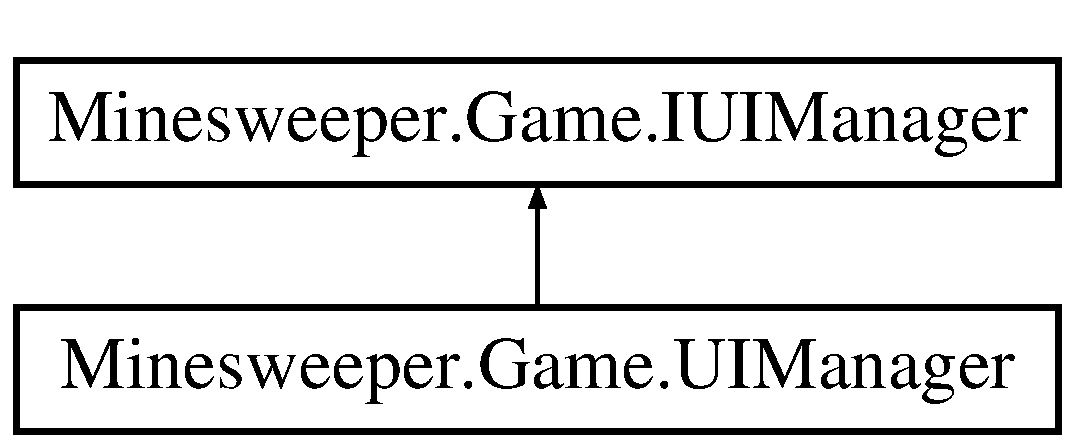
\includegraphics[height=2.000000cm]{class_minesweeper_1_1_game_1_1_u_i_manager}
\end{center}
\end{figure}
\subsection*{Public Member Functions}
\begin{DoxyCompactItemize}
\item 
\hyperlink{class_minesweeper_1_1_game_1_1_u_i_manager_a424a2a585050b3c85d119d84c4ba2b80}{U\+I\+Manager} ()
\begin{DoxyCompactList}\small\item\em Initializes a new instance of the \hyperlink{class_minesweeper_1_1_game_1_1_u_i_manager}{U\+I\+Manager} class with default Console\+Renderer and Console\+Reader. \end{DoxyCompactList}\item 
\hyperlink{class_minesweeper_1_1_game_1_1_u_i_manager_a996444e4a3c298158ab07d21f48c7307}{U\+I\+Manager} (\hyperlink{interface_minesweeper_1_1_lib_1_1_i_renderer}{I\+Renderer} renderer, \hyperlink{interface_minesweeper_1_1_lib_1_1_i_user_input_reader}{I\+User\+Input\+Reader} input\+Reader)
\begin{DoxyCompactList}\small\item\em Initializes a new instance of the \hyperlink{class_minesweeper_1_1_game_1_1_u_i_manager}{U\+I\+Manager} class. \end{DoxyCompactList}\item 
void \hyperlink{class_minesweeper_1_1_game_1_1_u_i_manager_a854a5ddce1304981c194c0a98d1d9f8c}{Display\+Intro} (string msg)
\begin{DoxyCompactList}\small\item\em Displays the introduction text of the game. \end{DoxyCompactList}\item 
void \hyperlink{class_minesweeper_1_1_game_1_1_u_i_manager_a32460cc4c19947d1b2f0724a11c1d47c}{Display\+End} (string message, int number\+Of\+Opened\+Cells)
\begin{DoxyCompactList}\small\item\em Displays the ending messages of the game. \end{DoxyCompactList}\item 
void \hyperlink{class_minesweeper_1_1_game_1_1_u_i_manager_a8ff1e458e0f14038b0abb9a44fa078a6}{Good\+Bye} (string good\+Bye\+Msg)
\begin{DoxyCompactList}\small\item\em Displays the messages when the user quits the game. \end{DoxyCompactList}\item 
void \hyperlink{class_minesweeper_1_1_game_1_1_u_i_manager_a2f3537e693d8efc90cbef90a0a63d34b}{Display\+High\+Scores} (I\+Enumerable$<$ Key\+Value\+Pair$<$ string, int $>$$>$ top\+Scores)
\begin{DoxyCompactList}\small\item\em Displays the high scores. \end{DoxyCompactList}\item 
void \hyperlink{class_minesweeper_1_1_game_1_1_u_i_manager_a67f57db959d9eff2829e1c3c64fb726f}{Display\+Error} (string error\+Msg)
\begin{DoxyCompactList}\small\item\em Displays error messages. \end{DoxyCompactList}\item 
string \hyperlink{class_minesweeper_1_1_game_1_1_u_i_manager_abf069aaf0ff743c8b5f27ea3dba46be4}{Read\+Input} ()
\begin{DoxyCompactList}\small\item\em Reads input from the user. \end{DoxyCompactList}\item 
void \hyperlink{class_minesweeper_1_1_game_1_1_u_i_manager_a4e433f59e1f0787aa4d69683b381dcfe}{Draw\+Table} (int minefield\+Rows, int minefield\+Cols)
\begin{DoxyCompactList}\small\item\em Draws the game table. \end{DoxyCompactList}\item 
void \hyperlink{class_minesweeper_1_1_game_1_1_u_i_manager_acc84e19d875400108a4026cf2861c5d9}{Clear\+Command\+Line} (string command\+Prompt)
\begin{DoxyCompactList}\small\item\em Clears the command line. \end{DoxyCompactList}\item 
void \hyperlink{class_minesweeper_1_1_game_1_1_u_i_manager_af1af79047deb6ba4ec6902a481df1c3e}{Draw\+Game\+Field} (\hyperlink{namespace_minesweeper_adf92d608047dafd69d16008492d317bd}{Cell\+Image}\mbox{[},\mbox{]} minefield, int\mbox{[},\mbox{]} neighbor\+Mines)
\begin{DoxyCompactList}\small\item\em Draws the game field. \end{DoxyCompactList}\end{DoxyCompactItemize}


\subsection{Detailed Description}
User Interface Manager class. 



\subsection{Constructor \& Destructor Documentation}
\hypertarget{class_minesweeper_1_1_game_1_1_u_i_manager_a424a2a585050b3c85d119d84c4ba2b80}{\index{Minesweeper\+::\+Game\+::\+U\+I\+Manager@{Minesweeper\+::\+Game\+::\+U\+I\+Manager}!U\+I\+Manager@{U\+I\+Manager}}
\index{U\+I\+Manager@{U\+I\+Manager}!Minesweeper\+::\+Game\+::\+U\+I\+Manager@{Minesweeper\+::\+Game\+::\+U\+I\+Manager}}
\subsubsection[{U\+I\+Manager}]{\setlength{\rightskip}{0pt plus 5cm}Minesweeper.\+Game.\+U\+I\+Manager.\+U\+I\+Manager (
\begin{DoxyParamCaption}
{}
\end{DoxyParamCaption}
)}}\label{class_minesweeper_1_1_game_1_1_u_i_manager_a424a2a585050b3c85d119d84c4ba2b80}


Initializes a new instance of the \hyperlink{class_minesweeper_1_1_game_1_1_u_i_manager}{U\+I\+Manager} class with default Console\+Renderer and Console\+Reader. 

\hypertarget{class_minesweeper_1_1_game_1_1_u_i_manager_a996444e4a3c298158ab07d21f48c7307}{\index{Minesweeper\+::\+Game\+::\+U\+I\+Manager@{Minesweeper\+::\+Game\+::\+U\+I\+Manager}!U\+I\+Manager@{U\+I\+Manager}}
\index{U\+I\+Manager@{U\+I\+Manager}!Minesweeper\+::\+Game\+::\+U\+I\+Manager@{Minesweeper\+::\+Game\+::\+U\+I\+Manager}}
\subsubsection[{U\+I\+Manager}]{\setlength{\rightskip}{0pt plus 5cm}Minesweeper.\+Game.\+U\+I\+Manager.\+U\+I\+Manager (
\begin{DoxyParamCaption}
\item[{{\bf I\+Renderer}}]{renderer, }
\item[{{\bf I\+User\+Input\+Reader}}]{input\+Reader}
\end{DoxyParamCaption}
)}}\label{class_minesweeper_1_1_game_1_1_u_i_manager_a996444e4a3c298158ab07d21f48c7307}


Initializes a new instance of the \hyperlink{class_minesweeper_1_1_game_1_1_u_i_manager}{U\+I\+Manager} class. 


\begin{DoxyParams}{Parameters}
{\em renderer} & The renderer which is going to be used by the \hyperlink{class_minesweeper_1_1_game_1_1_u_i_manager}{U\+I\+Manager}.\\
\hline
{\em input\+Reader} & The input reader which \hyperlink{class_minesweeper_1_1_game_1_1_u_i_manager}{U\+I\+Manager} is going to use.\\
\hline
\end{DoxyParams}


\subsection{Member Function Documentation}
\hypertarget{class_minesweeper_1_1_game_1_1_u_i_manager_acc84e19d875400108a4026cf2861c5d9}{\index{Minesweeper\+::\+Game\+::\+U\+I\+Manager@{Minesweeper\+::\+Game\+::\+U\+I\+Manager}!Clear\+Command\+Line@{Clear\+Command\+Line}}
\index{Clear\+Command\+Line@{Clear\+Command\+Line}!Minesweeper\+::\+Game\+::\+U\+I\+Manager@{Minesweeper\+::\+Game\+::\+U\+I\+Manager}}
\subsubsection[{Clear\+Command\+Line}]{\setlength{\rightskip}{0pt plus 5cm}void Minesweeper.\+Game.\+U\+I\+Manager.\+Clear\+Command\+Line (
\begin{DoxyParamCaption}
\item[{string}]{command\+Prompt}
\end{DoxyParamCaption}
)}}\label{class_minesweeper_1_1_game_1_1_u_i_manager_acc84e19d875400108a4026cf2861c5d9}


Clears the command line. 


\begin{DoxyParams}{Parameters}
{\em command\+Prompt} & The prompt that is going to be shown to the user.\\
\hline
\end{DoxyParams}


Implements \hyperlink{interface_minesweeper_1_1_game_1_1_i_u_i_manager_aafbe4485c18fe5dd0269a1a54599d1fc}{Minesweeper.\+Game.\+I\+U\+I\+Manager}.

\hypertarget{class_minesweeper_1_1_game_1_1_u_i_manager_a32460cc4c19947d1b2f0724a11c1d47c}{\index{Minesweeper\+::\+Game\+::\+U\+I\+Manager@{Minesweeper\+::\+Game\+::\+U\+I\+Manager}!Display\+End@{Display\+End}}
\index{Display\+End@{Display\+End}!Minesweeper\+::\+Game\+::\+U\+I\+Manager@{Minesweeper\+::\+Game\+::\+U\+I\+Manager}}
\subsubsection[{Display\+End}]{\setlength{\rightskip}{0pt plus 5cm}void Minesweeper.\+Game.\+U\+I\+Manager.\+Display\+End (
\begin{DoxyParamCaption}
\item[{string}]{message, }
\item[{int}]{number\+Of\+Opened\+Cells}
\end{DoxyParamCaption}
)}}\label{class_minesweeper_1_1_game_1_1_u_i_manager_a32460cc4c19947d1b2f0724a11c1d47c}


Displays the ending messages of the game. 


\begin{DoxyParams}{Parameters}
{\em message} & The ending message.\\
\hline
{\em number\+Of\+Opened\+Cells} & The number of cells the user opened during the game.\\
\hline
\end{DoxyParams}


Implements \hyperlink{interface_minesweeper_1_1_game_1_1_i_u_i_manager_a7df49d712d01db2b9e9b36218667cc23}{Minesweeper.\+Game.\+I\+U\+I\+Manager}.

\hypertarget{class_minesweeper_1_1_game_1_1_u_i_manager_a67f57db959d9eff2829e1c3c64fb726f}{\index{Minesweeper\+::\+Game\+::\+U\+I\+Manager@{Minesweeper\+::\+Game\+::\+U\+I\+Manager}!Display\+Error@{Display\+Error}}
\index{Display\+Error@{Display\+Error}!Minesweeper\+::\+Game\+::\+U\+I\+Manager@{Minesweeper\+::\+Game\+::\+U\+I\+Manager}}
\subsubsection[{Display\+Error}]{\setlength{\rightskip}{0pt plus 5cm}void Minesweeper.\+Game.\+U\+I\+Manager.\+Display\+Error (
\begin{DoxyParamCaption}
\item[{string}]{error\+Msg}
\end{DoxyParamCaption}
)}}\label{class_minesweeper_1_1_game_1_1_u_i_manager_a67f57db959d9eff2829e1c3c64fb726f}


Displays error messages. 


\begin{DoxyParams}{Parameters}
{\em error\+Msg} & The error message to be displayed.\\
\hline
\end{DoxyParams}


Implements \hyperlink{interface_minesweeper_1_1_game_1_1_i_u_i_manager_afa8d49b68057b38c302d945c829e1856}{Minesweeper.\+Game.\+I\+U\+I\+Manager}.

\hypertarget{class_minesweeper_1_1_game_1_1_u_i_manager_a2f3537e693d8efc90cbef90a0a63d34b}{\index{Minesweeper\+::\+Game\+::\+U\+I\+Manager@{Minesweeper\+::\+Game\+::\+U\+I\+Manager}!Display\+High\+Scores@{Display\+High\+Scores}}
\index{Display\+High\+Scores@{Display\+High\+Scores}!Minesweeper\+::\+Game\+::\+U\+I\+Manager@{Minesweeper\+::\+Game\+::\+U\+I\+Manager}}
\subsubsection[{Display\+High\+Scores}]{\setlength{\rightskip}{0pt plus 5cm}void Minesweeper.\+Game.\+U\+I\+Manager.\+Display\+High\+Scores (
\begin{DoxyParamCaption}
\item[{I\+Enumerable$<$ Key\+Value\+Pair$<$ string, int $>$$>$}]{top\+Scores}
\end{DoxyParamCaption}
)}}\label{class_minesweeper_1_1_game_1_1_u_i_manager_a2f3537e693d8efc90cbef90a0a63d34b}


Displays the high scores. 


\begin{DoxyParams}{Parameters}
{\em top\+Scores} & The top scores to be displayed.\\
\hline
\end{DoxyParams}


Implements \hyperlink{interface_minesweeper_1_1_game_1_1_i_u_i_manager_a562c29c1904a923494c26511e0a6a3d8}{Minesweeper.\+Game.\+I\+U\+I\+Manager}.

\hypertarget{class_minesweeper_1_1_game_1_1_u_i_manager_a854a5ddce1304981c194c0a98d1d9f8c}{\index{Minesweeper\+::\+Game\+::\+U\+I\+Manager@{Minesweeper\+::\+Game\+::\+U\+I\+Manager}!Display\+Intro@{Display\+Intro}}
\index{Display\+Intro@{Display\+Intro}!Minesweeper\+::\+Game\+::\+U\+I\+Manager@{Minesweeper\+::\+Game\+::\+U\+I\+Manager}}
\subsubsection[{Display\+Intro}]{\setlength{\rightskip}{0pt plus 5cm}void Minesweeper.\+Game.\+U\+I\+Manager.\+Display\+Intro (
\begin{DoxyParamCaption}
\item[{string}]{msg}
\end{DoxyParamCaption}
)}}\label{class_minesweeper_1_1_game_1_1_u_i_manager_a854a5ddce1304981c194c0a98d1d9f8c}


Displays the introduction text of the game. 


\begin{DoxyParams}{Parameters}
{\em msg} & The introduction message.\\
\hline
\end{DoxyParams}


Implements \hyperlink{interface_minesweeper_1_1_game_1_1_i_u_i_manager_a0a8ff25e5b1a5013bdbf2c5b7a5f82c3}{Minesweeper.\+Game.\+I\+U\+I\+Manager}.

\hypertarget{class_minesweeper_1_1_game_1_1_u_i_manager_af1af79047deb6ba4ec6902a481df1c3e}{\index{Minesweeper\+::\+Game\+::\+U\+I\+Manager@{Minesweeper\+::\+Game\+::\+U\+I\+Manager}!Draw\+Game\+Field@{Draw\+Game\+Field}}
\index{Draw\+Game\+Field@{Draw\+Game\+Field}!Minesweeper\+::\+Game\+::\+U\+I\+Manager@{Minesweeper\+::\+Game\+::\+U\+I\+Manager}}
\subsubsection[{Draw\+Game\+Field}]{\setlength{\rightskip}{0pt plus 5cm}void Minesweeper.\+Game.\+U\+I\+Manager.\+Draw\+Game\+Field (
\begin{DoxyParamCaption}
\item[{{\bf Cell\+Image}}]{minefield\mbox{[},\mbox{]}, }
\item[{int}]{neighbor\+Mines\mbox{[},\mbox{]}}
\end{DoxyParamCaption}
)}}\label{class_minesweeper_1_1_game_1_1_u_i_manager_af1af79047deb6ba4ec6902a481df1c3e}


Draws the game field. 


\begin{DoxyParams}{Parameters}
{\em minefield} & The minefield to be drawn.\\
\hline
{\em neighbor\+Mines} & The minefield with all values of neighboring mines.\\
\hline
\end{DoxyParams}


Implements \hyperlink{interface_minesweeper_1_1_game_1_1_i_u_i_manager_acae1778c1bdc80065c2b18afb1d11a70}{Minesweeper.\+Game.\+I\+U\+I\+Manager}.

\hypertarget{class_minesweeper_1_1_game_1_1_u_i_manager_a4e433f59e1f0787aa4d69683b381dcfe}{\index{Minesweeper\+::\+Game\+::\+U\+I\+Manager@{Minesweeper\+::\+Game\+::\+U\+I\+Manager}!Draw\+Table@{Draw\+Table}}
\index{Draw\+Table@{Draw\+Table}!Minesweeper\+::\+Game\+::\+U\+I\+Manager@{Minesweeper\+::\+Game\+::\+U\+I\+Manager}}
\subsubsection[{Draw\+Table}]{\setlength{\rightskip}{0pt plus 5cm}void Minesweeper.\+Game.\+U\+I\+Manager.\+Draw\+Table (
\begin{DoxyParamCaption}
\item[{int}]{minefield\+Rows, }
\item[{int}]{minefield\+Cols}
\end{DoxyParamCaption}
)}}\label{class_minesweeper_1_1_game_1_1_u_i_manager_a4e433f59e1f0787aa4d69683b381dcfe}


Draws the game table. 


\begin{DoxyParams}{Parameters}
{\em minefield\+Rows} & The count of the minefield rows.\\
\hline
{\em minefield\+Cols} & The count of the minefield columns.\\
\hline
\end{DoxyParams}


Implements \hyperlink{interface_minesweeper_1_1_game_1_1_i_u_i_manager_a0dd9d9e47eba3707562cf1493a9bf6aa}{Minesweeper.\+Game.\+I\+U\+I\+Manager}.

\hypertarget{class_minesweeper_1_1_game_1_1_u_i_manager_a8ff1e458e0f14038b0abb9a44fa078a6}{\index{Minesweeper\+::\+Game\+::\+U\+I\+Manager@{Minesweeper\+::\+Game\+::\+U\+I\+Manager}!Good\+Bye@{Good\+Bye}}
\index{Good\+Bye@{Good\+Bye}!Minesweeper\+::\+Game\+::\+U\+I\+Manager@{Minesweeper\+::\+Game\+::\+U\+I\+Manager}}
\subsubsection[{Good\+Bye}]{\setlength{\rightskip}{0pt plus 5cm}void Minesweeper.\+Game.\+U\+I\+Manager.\+Good\+Bye (
\begin{DoxyParamCaption}
\item[{string}]{good\+Bye\+Msg}
\end{DoxyParamCaption}
)}}\label{class_minesweeper_1_1_game_1_1_u_i_manager_a8ff1e458e0f14038b0abb9a44fa078a6}


Displays the messages when the user quits the game. 


\begin{DoxyParams}{Parameters}
{\em good\+Bye\+Msg} & The goodbye message.\\
\hline
\end{DoxyParams}


Implements \hyperlink{interface_minesweeper_1_1_game_1_1_i_u_i_manager_a61f1153446f2f52f258363ccd9008c20}{Minesweeper.\+Game.\+I\+U\+I\+Manager}.

\hypertarget{class_minesweeper_1_1_game_1_1_u_i_manager_abf069aaf0ff743c8b5f27ea3dba46be4}{\index{Minesweeper\+::\+Game\+::\+U\+I\+Manager@{Minesweeper\+::\+Game\+::\+U\+I\+Manager}!Read\+Input@{Read\+Input}}
\index{Read\+Input@{Read\+Input}!Minesweeper\+::\+Game\+::\+U\+I\+Manager@{Minesweeper\+::\+Game\+::\+U\+I\+Manager}}
\subsubsection[{Read\+Input}]{\setlength{\rightskip}{0pt plus 5cm}string Minesweeper.\+Game.\+U\+I\+Manager.\+Read\+Input (
\begin{DoxyParamCaption}
{}
\end{DoxyParamCaption}
)}}\label{class_minesweeper_1_1_game_1_1_u_i_manager_abf069aaf0ff743c8b5f27ea3dba46be4}


Reads input from the user. 

\begin{DoxyReturn}{Returns}
The user input.
\end{DoxyReturn}


Implements \hyperlink{interface_minesweeper_1_1_game_1_1_i_u_i_manager_ac2d51aed7d1d677c899fa596becc6afb}{Minesweeper.\+Game.\+I\+U\+I\+Manager}.



The documentation for this class was generated from the following file\+:\begin{DoxyCompactItemize}
\item 
Minesweeper/\+Minesweeper/\+Minesweeper.\+game/U\+I\+Manager.\+cs\end{DoxyCompactItemize}

\hypertarget{class_minesweeper_1_1_unit_tests_1_1_game_1_1_u_i_manager_test}{\section{Minesweeper.\+Unit\+Tests.\+Game.\+U\+I\+Manager\+Test Class Reference}
\label{class_minesweeper_1_1_unit_tests_1_1_game_1_1_u_i_manager_test}\index{Minesweeper.\+Unit\+Tests.\+Game.\+U\+I\+Manager\+Test@{Minesweeper.\+Unit\+Tests.\+Game.\+U\+I\+Manager\+Test}}
}
\subsection*{Public Member Functions}
\begin{DoxyCompactItemize}
\item 
\hypertarget{class_minesweeper_1_1_unit_tests_1_1_game_1_1_u_i_manager_test_a27d6d58ca5723300d0499d4175184a09}{void {\bfseries Display\+Intro\+Should\+Print\+In\+The\+Console\+Proper\+Message} ()}\label{class_minesweeper_1_1_unit_tests_1_1_game_1_1_u_i_manager_test_a27d6d58ca5723300d0499d4175184a09}

\item 
\hypertarget{class_minesweeper_1_1_unit_tests_1_1_game_1_1_u_i_manager_test_ae378eb70da7d6c8bb8a61172b3cf1ede}{void {\bfseries Display\+Intro\+When\+Message\+Is\+Null\+Should\+Throw\+An\+Exception} ()}\label{class_minesweeper_1_1_unit_tests_1_1_game_1_1_u_i_manager_test_ae378eb70da7d6c8bb8a61172b3cf1ede}

\item 
\hypertarget{class_minesweeper_1_1_unit_tests_1_1_game_1_1_u_i_manager_test_a930b1aad92fdc0ab3dfef625eb37d450}{void {\bfseries Display\+End\+Should\+Print\+In\+The\+Console\+Proper\+Message} ()}\label{class_minesweeper_1_1_unit_tests_1_1_game_1_1_u_i_manager_test_a930b1aad92fdc0ab3dfef625eb37d450}

\item 
\hypertarget{class_minesweeper_1_1_unit_tests_1_1_game_1_1_u_i_manager_test_a7f0fde3bc39476048907edf038984c4f}{void {\bfseries Display\+End\+When\+Opened\+Cells\+Is\+Negative\+Should\+Throw\+An\+Exception} ()}\label{class_minesweeper_1_1_unit_tests_1_1_game_1_1_u_i_manager_test_a7f0fde3bc39476048907edf038984c4f}

\item 
\hypertarget{class_minesweeper_1_1_unit_tests_1_1_game_1_1_u_i_manager_test_a19a0a251d428e09e0f4e37142d53e7b9}{void {\bfseries Display\+End\+When\+Message\+Is\+Null\+Should\+Throw\+An\+Exception} ()}\label{class_minesweeper_1_1_unit_tests_1_1_game_1_1_u_i_manager_test_a19a0a251d428e09e0f4e37142d53e7b9}

\item 
\hypertarget{class_minesweeper_1_1_unit_tests_1_1_game_1_1_u_i_manager_test_a10a158aaef78f4cd5ffa34d4ee37383b}{void {\bfseries Display\+End\+When\+Message\+Is\+Empty\+Should\+Throw\+An\+Exception} ()}\label{class_minesweeper_1_1_unit_tests_1_1_game_1_1_u_i_manager_test_a10a158aaef78f4cd5ffa34d4ee37383b}

\item 
\hypertarget{class_minesweeper_1_1_unit_tests_1_1_game_1_1_u_i_manager_test_ae8c434a0a6f0122305be9243ffc89113}{void {\bfseries Good\+Bye\+Should\+Print\+In\+The\+Console\+Proper\+Message} ()}\label{class_minesweeper_1_1_unit_tests_1_1_game_1_1_u_i_manager_test_ae8c434a0a6f0122305be9243ffc89113}

\item 
\hypertarget{class_minesweeper_1_1_unit_tests_1_1_game_1_1_u_i_manager_test_a2aaf2f56748c63fc415270a0dca71e73}{void {\bfseries Good\+Bye\+When\+Message\+Is\+Null\+Should\+Throw\+An\+Exception} ()}\label{class_minesweeper_1_1_unit_tests_1_1_game_1_1_u_i_manager_test_a2aaf2f56748c63fc415270a0dca71e73}

\item 
\hypertarget{class_minesweeper_1_1_unit_tests_1_1_game_1_1_u_i_manager_test_aa3e6d09173cd088d2e6b6fed42a724d3}{void {\bfseries Display\+Error\+Should\+Print\+In\+The\+Console\+Proper\+Message} ()}\label{class_minesweeper_1_1_unit_tests_1_1_game_1_1_u_i_manager_test_aa3e6d09173cd088d2e6b6fed42a724d3}

\item 
\hypertarget{class_minesweeper_1_1_unit_tests_1_1_game_1_1_u_i_manager_test_ae664d293a4d7540900737e632a69e4f8}{void {\bfseries Display\+Error\+Should\+Call\+Renderer\+Correctly} ()}\label{class_minesweeper_1_1_unit_tests_1_1_game_1_1_u_i_manager_test_ae664d293a4d7540900737e632a69e4f8}

\item 
\hypertarget{class_minesweeper_1_1_unit_tests_1_1_game_1_1_u_i_manager_test_a733a53d44b88edd65b980dc0a53569f8}{void {\bfseries Display\+Error\+When\+Message\+Is\+Empty\+Should\+Throw\+An\+Exception} ()}\label{class_minesweeper_1_1_unit_tests_1_1_game_1_1_u_i_manager_test_a733a53d44b88edd65b980dc0a53569f8}

\item 
\hypertarget{class_minesweeper_1_1_unit_tests_1_1_game_1_1_u_i_manager_test_a8e65c909b924e62e1f4f4d2d98ef03e2}{void {\bfseries Display\+Error\+When\+Message\+Is\+Null\+Should\+Throw\+An\+Exception} ()}\label{class_minesweeper_1_1_unit_tests_1_1_game_1_1_u_i_manager_test_a8e65c909b924e62e1f4f4d2d98ef03e2}

\item 
\hypertarget{class_minesweeper_1_1_unit_tests_1_1_game_1_1_u_i_manager_test_a8e6c3136537d37b82c6b3daf59d56bb3}{void {\bfseries Display\+High\+Scores\+When\+Argument\+Is\+Null\+Should\+Throw\+An\+Exception} ()}\label{class_minesweeper_1_1_unit_tests_1_1_game_1_1_u_i_manager_test_a8e6c3136537d37b82c6b3daf59d56bb3}

\item 
\hypertarget{class_minesweeper_1_1_unit_tests_1_1_game_1_1_u_i_manager_test_a8b1a2dbef62b42a328c60fc5bd42040d}{void {\bfseries Display\+High\+Scores\+Should\+Print\+Proper\+List\+In\+The\+Console} ()}\label{class_minesweeper_1_1_unit_tests_1_1_game_1_1_u_i_manager_test_a8b1a2dbef62b42a328c60fc5bd42040d}

\item 
\hypertarget{class_minesweeper_1_1_unit_tests_1_1_game_1_1_u_i_manager_test_a508682d8da77a4e9f1fba7a96d11d36a}{void {\bfseries Clear\+Command\+Line\+With\+Null\+Parameter\+Should\+Throw\+An\+Exception} ()}\label{class_minesweeper_1_1_unit_tests_1_1_game_1_1_u_i_manager_test_a508682d8da77a4e9f1fba7a96d11d36a}

\item 
\hypertarget{class_minesweeper_1_1_unit_tests_1_1_game_1_1_u_i_manager_test_a34a6e403b0fe20e494342a1b746999c2}{void {\bfseries Draw\+Game\+Field\+With\+Different\+Matrices\+By\+Size\+Should\+Throw\+An\+Exception} ()}\label{class_minesweeper_1_1_unit_tests_1_1_game_1_1_u_i_manager_test_a34a6e403b0fe20e494342a1b746999c2}

\item 
\hypertarget{class_minesweeper_1_1_unit_tests_1_1_game_1_1_u_i_manager_test_ad343db56504a5850b0e27d9ed6a4fafa}{void {\bfseries Test\+Read\+Name} ()}\label{class_minesweeper_1_1_unit_tests_1_1_game_1_1_u_i_manager_test_ad343db56504a5850b0e27d9ed6a4fafa}

\end{DoxyCompactItemize}
\subsection*{Static Public Member Functions}
\begin{DoxyCompactItemize}
\item 
\hypertarget{class_minesweeper_1_1_unit_tests_1_1_game_1_1_u_i_manager_test_a6e798aa81cb723e138dfc4205b9eceba}{static void {\bfseries Class\+Initialization} (Test\+Context ctx)}\label{class_minesweeper_1_1_unit_tests_1_1_game_1_1_u_i_manager_test_a6e798aa81cb723e138dfc4205b9eceba}

\end{DoxyCompactItemize}


The documentation for this class was generated from the following file\+:\begin{DoxyCompactItemize}
\item 
Minesweeper/\+Minesweeper/\+Minesweeper.\+Unit\+Tests/\+Game/U\+I\+Manager\+Test.\+cs\end{DoxyCompactItemize}

%--- End generated contents ---

% Index
\newpage
\phantomsection
\addcontentsline{toc}{chapter}{Index}
\printindex

\end{document}
